\documentclass[%
%%% PARA ESCOLHER O ESTILO TIRE O SIMBOLO %(COMENTÁRIO)
%SemVinculoColorido,
%SemFormatacaoCapitulo,
%SemFolhaAprovacao,
%SemImagens,
%CitacaoNumerica, %% o padrão é citação tipo autor-data
%PublicacaoDissOuTese, %% (é também o "default") com ficha catal. e folha de aprovação em branco. Caso tenha lista de símbolos e lista de siglas e abreviaturas retirar os comentários dos arquivos siglas.tex e abreviaturasesiglas.tex. Retirar também os comentários indicados nesse arquivo, nos includes
%PublicacaoArtigoOuRelatorio, %% texto sequencial, sem quebra de páginas nem folhas em branco
PublicacaoProposta, %% igual tese/dissertação, mas sem ficha catal. e fol. de aprov.
%PublicacaoLivro, %% com capítulos
%PublicacaoLivro,SemFormatacaoCapitulo, %% sem capítulos
english,portuguese %% para os documentos em Português com abstract.tex em Inglês
%portuguese,english %% para os documentos em Inglês com abstract.tex em Português
,LogoINPE% comentar essa linha para fazer aparecer o logo do Governo
,CCBYNC	% as opções de licença são: CCBY, CCBYSA, CCBYND, CCBYNC, CCBYNCSA, CCBYNCND, GPLv3 e INPECopyright
]{tdiinpe}
%]{../../../../../iconet.com.br/banon/2008/03.25.01.19/doc/tdiinpe}

% PARA EXIBIR EM ARIAL TIRAR O COMENTÁRIO DAS DUAS LINHAS SEGUINTES
%\renewcommand{\rmdefault}{phv} % Arial
%\renewcommand{\sfdefault}{phv} % Arial

% PARA PUBLICAÇÕES EM INGLÊS:
% renomear o arquivo: abnt-alf.bst para abnt-alfportuguese.bst
% renomear o arquivo: abnt-alfenglish.bst para abnt-alf.bst


%%%%%%%%%%%%%%%%%%%%%%%%%%%%%%%%%%%%%%%%%%%%%
%%% Pacotes já previamente carregados:      %
%%%%%%%%%%%%%%%%%%%%%%%%%%%%%%%%%%%%%%%%%%%%%%%%%%%%%%%%%%%%%%%%%%%%%%%%
%%% ifthen,calc,graphicx,color,inputenc,babel,hyphenat,array,setspace, %
%%% bigdelim,multirow,supertabular,tabularx,longtable,lastpage,lscape, %
%%% rotate,caption2,amsmath,amssymb,amsthm,subfigure,tocloft,makeidx,  %
%%% eso-pic,calligra,hyperref,ae,fontenc                               %
%%%%%%%%%%%%%%%%%%%%%%%%%%%%%%%%%%%%%%%%%%%%%%%%%%%%%%%%%%%%%%%%%%%%%%%%
%%% insira neste campo, comandos de LaTeX %%%
%%% \usepackage{_exemplo_}
% etc.
%%%%%%%%%%%%%%%%%%%%%%%%%%%%%%%%%%%%%%%%%%%%%

%\watermark{Revisão No. ##} %% use o comando \watermark para identificar a versão de seu documento
%% comente este comando quando for gerar a versão final
\usepackage{rotating}
\usepackage{dsfont}
\usepackage{comment}
%%%%%%%%%%%%%%%%%%%CAPA%%%%%%%%%%%%%%%%%%%%%%%%%%%%%%%%
%\serieinpe{INPE-NNNNN-TDI/NNNN} %% não mais usado

\titulo{Escrever o título no idioma em que foi escrito a publicação}
\title{Escrever o título em Inglês para publicações escritas em Português e em Português para publicações escritas em Inglês} %% 
\author{Nome Completo do Autor1\\Nome Completo do Autor2} %% coloque o nome do(s) autor(es)
\descriccao{Tese de Doutorado ou Dissertação de Mestrado do Curso de Pós-Graduação em Nome do Curso, orientada pelo(a) Dr(a). Nome do Orientador(a), aprovada em dd de mês por extenso de aaaa.}
\repositorio{aa/bb/cc/dd} %% repositório onde está depositado este documento - na omissão, será preenchido pelo SID
\tipoDaPublicacao{TDI}	%% tipo da publicação (NTC, RPQ, PRP, MAN, PUD, TDI, TAE e PRE) na ausência do número de série INPE, caso contrário deixar vazio
\IBI{xx/yy} %% IBI (exemplo: J8LNKAN8PW/36CT2G2) quando existir, caso contrário o nome do repositório onde está depositado o documento

\date{AAAA}%ano da publicação

%%%%%%%%%%%%%%%%%%%%%%%%%%VERSO DA CAPA%%%%%%%%%%%%%%%%%%%%%%%%%%%%%%%%%%%%%%%%%%%%%%%
\tituloverso{\vspace{-0.9cm}\textbf{\PublicadoPor:}}
\descriccaoverso{Instituto Nacional de Pesquisas Espaciais - INPE\\
Gabinete do Diretor (GB)\\
Serviço de Informação e Documentação (SID)\\
Caixa Postal 515 - CEP 12.245-970\\
São José dos Campos - SP - Brasil\\
Tel.:(012) 3945-6923/6921\\
Fax: (012) 3945-6919\\
E-mail: {\url{pubtc@sid.inpe.br}}
}

\descriccaoversoA{\textbf{\ConselhoDeEditoracao:}\\
\textbf{\Presidente:}\\
Marciana Leite Ribeiro - Serviço de Informação e Documentação (SID)\\
\textbf{\Membros:}\\
Dr. Gerald Jean Francis Banon - Coordenação Observação da Terra (OBT)\\
Dr. Amauri Silva Montes - Coordenação Engenharia e Tecnologia Espaciais (ETE)\\
Dr. André de Castro Milone - Coordenação Ciências Espaciais e Atmosféricas (CEA)\\
Dr. Joaquim José Barroso de Castro -  Centro de Tecnologias Espaciais (CTE)\\
Dr. Manoel Alonso Gan - Centro de Previsão de Tempo e Estudos Climáticos (CPT)\\
Drª Maria do Carmo de Andrade Nono - Conselho de Pós-Graduação\\
Dr. Plínio Carlos Alvalá - Centro de Ciência do Sistema Terrestre (CST)\\
\textbf{\BibliotecaDigital:}\\
Dr. Gerald Jean Francis Banon - Coordenação de Observação da Terra (OBT)\\
Clayton Martins Pereira - Serviço de Informação e Documentação (SID)\\
%Jefferson Andrade Ancelmo - Serviço de Informação e Documentação (SID)\\
%Simone A. Del-Ducca Barbedo - Serviço de Informação e Documentação (SID)\\
%Deicy Farabello - Centro de Previsão de Tempo  e Estudos Climáticos (CPT)\\
\textbf{\RevisaoNormalizacaoDocumentaria:}\\
Simone Angélica Del Ducca Barbedo - Serviço de Informação e Documentação (SID) \\
%Marilúcia Santos Melo Cid - Serviço de Informação e Documentação (SID)\\
Yolanda Ribeiro da Silva Souza - Serviço de Informação e Documentação (SID)\\
\textbf{\EditoracaoEletronica:}\\
Marcelo de Castro Pazos - Serviço de Informação e Documentação (SID)\\
André Luis Dias Fernandes - Serviço de Informação e Documentação (SID)\\
}

%%%%%%%%%%%%%%%%%%%FOLHA DE ROSTO

%%%%%%%%%%%%%%%FICHA CATALOGRÁFICA
%% NÃO PREENCHER - SERÁ PREENCHIDO PELO SID

\cutterFICHAC{Cutter}
\autorUltimoNomeFICHAC{Sobrenome, Nomes} %% exemplo: Fuckner, Marcus André
\autorFICHAC {Nome Completo do Autor1; Nome Completo do Autor2} %% Campo opcional (se não usado prevalece \author)
\tituloFICHAC{Titulo da publicação}
\instituicaosigla{INPE}
\instituicaocidade{São José dos Campos}
\paginasFICHAC{\pageref{numeroDePáginasDoPretexto} + \pageref{LastPage}} %% número total de páginas
%\serieinpe{INPE-00000-TDI/0000} %% não mais usado
\palavraschaveFICHAC{1.~Palavra chave. 2.~Palavra chave 3.~Palavra chave. 4.~Palavra chave. 5.~Palavra chave  I.~\mbox{Título}.} %% recomenda-se pelo menos 5 palavras-chaves - \mbox{} é para evitar hifenização 
\numeroCDUFICHAC{000.000} %% número do CDU 

% Nota da ficha (para TD)
\tipoTD{Dissertação ou Tese} % Dissertação ou Tese
\cursoFA{Mestrado ou Doutorado em Nome do Curso}
\instituicaoDefesa{Instituto Nacional de Pesquisas Espaciais}
\anoDefesa{AAAA} % ano de defesa 
\nomeAtributoOrientadorFICHAC{Orientador}	% pode ser: Orientador, Orientadora ou Orientadores
\valorAtributoOrientadorFICHAC{José da Silva} % nome(s) completo(s)

%%%%%%%%%%%%%%%FOLHA DE APROVAÇAO PELA BANCA EXAMINADORA
\tituloFA{\textbf{ATENÇÃO! A FOLHA DE APROVAÇÃO SERÁ INCLUIDA POSTERIORMENTE.}}
%\cursoFA{\textbf{}}
\candidatoOUcandidataFA{}
\dataAprovacaoFA{}
\membroA{}{}{}
\membroB{}{}{}
\membroC{}{}{}
\membroD{}{}{}
\membroE{}{}{}
\membroF{}{}{}
\membroG{}{}{}
\ifpdf

%%%%%%%%%%%%%%NÍVEL DE COMPRESSÃO {0 -- 9}
\pdfcompresslevel 9
\fi
%%% define em 80% a largura das figuras %%%
\newlength{\mylenfig} 
\setlength{\mylenfig}{0.8\textwidth}
%%%%%%%%%%%%%%%%%%%%%%%%%%%%%%%%%%%%%%%%%%%

%%%%%%%%%%%%%%COMANDOS PESSOAIS
\newcommand{\vetor}[1]{\mathit{\mathbf{#1}}} %% faça as modificações pertinentes no arquivo configuracao.tex

\makeindex  %% não alterar, gera INDEX, caso haja algum termo indexado no texto

\begin{document} %% início do documento %% não mexer

%\marcaRegistrada{}	% comando opcional usado para informar abaixo da ficha catalográfica sobre marca registrada
\marcaRegistrada{Informar aqui sobre marca registrada (a modificação desta linha deve ser feita no arquivo publicacao.tex).}

\maketitle  %% não alterar, gera páginas obrigatórias (folha de rosto, ficha catalográfica e folha de aprovação), automaticamente

%%% Comente as linhas opcionais abaixo caso não as deseje
%%%%%%%%%%%%%%%%%%%%%%%%%%%%%%%%%%%%%%%%%%%%%%%%%%%%%%%%%%%%%%%%%%%%%%%%%%%%%%%%%
% Epígrafe %% opcional

\begin{epigrafe} %% insira sua epígrafe abaixo; estilo livre

\hypertarget{estilo:epigrafe}{} %% uso para este Guia
 
\textit{\large``A vida será mais complicada se você possuir uma curiosidade ativa, além de aumentarem as chances de você entrar em apuros, mas será mais divertida''.}

\vspace{1cm}

\hspace{4cm} \emph{\textsc{Edward Speyer}}\\\hspace{4cm} em \textsl{``Seis Caminhos a Partir de Newton''}, 1994

\end{epigrafe}
 %% Opcional
%%%%%%%%%%%%%%%%%%%%%%%%%%%%%%%%%%%%%%%%%%%%%%%%%%%%%%%%%%%%%%%%%%%%%%%%%%%%%%%%%
% Dedicatória %% opcional

\begin{dedicatoria} %% insira sua dedicatória abaixo; estilo livre

\hypertarget{estilo:dedicatoria}{} %% uso para este Guia
 
%% use 'a meus' em vez de 'aos meus', isto é, não use o artigo definido com pronomes possessivos

\newcommand{\mytext}{A meus pais \textbf{Nicanor} e \textbf{Jaci}, à minha irmã \textbf{Luciana} e ao meu esposo \textbf{William}}

\begin{comment}
%%% sugestão de estilo
\ifcalligra %% fonte calligra presente nas versões mais novas do MiKTeX (>= 2.4)
  \calligra\Large \mytext %% exemplo usando estilo de fonte caligráfica, caso haja
\else
	\itshape\Large \mytext 
\fi
\end{comment}

	\itshape\Large \mytext 

\end{dedicatoria} %% Opcional
%%%%%%%%%%%%%%%%%%%%%%%%%%%%%%%%%%%%%%%%%%%%%%%%%%%%%%%%%%%%%%%%%%%%%%%%%%%%%%%%%
% AGRADECIMENTOS %% opcional

\begin{agradecimentos}  %% insira abaixo seus agradecimentos

\hypertarget{estilo:agradecimentos}{} %% uso para este Guia

Primeiramente gostaria de agradecer a toda a minha família, sem a qual nada disso seria possível, em especial a minha mãe Xarlene e minha madrinha Araída por sempre acreditarem em mim, minha irmã favorita do mundo Natália, meu pai Irair, minhas avós Genoveva e Maria das Graças e meu padrasto Eudes.
Também a todos os inúmeros parentes que me acolheram de alguma forma, seja no Tocantins, em Goiás, no Distrito Federal ou em São Paulo.
Em especial ao meu avô Antônio Macena, que nos deixou muito cedo em um acidente logo após o início deste trabalho.

Ao Dr. Maurício, por me acolher no INPE, aceitado como aluno e me abrir as portas do CCS, meu sincero obrigado pela oportunidade e por todo o suporte que me forneceu.

Ao Dr. Rodrigo, por aceitar um completo desconhecido como aluno, e me ensinar tantas coisas sobre computação ao longo desse tempo, e pelos puxões de orelha merecidos.

Aos meus colegas Bruno e Gabriela que aceitaram dividir apartamento comigo, e me aguentarem por todo esse tempo.

Ao Ítalo, Isomar, Danilo e Johnathan pela amizade, tantos almoços compartilhados e por serem estarem disponíveis para uma conversa aleatória sobre algum conceito espacial obscuro de um manual da União Soviética dos anos 70.

As comissões organizadoras do WETE e do CubeDesign que me permitiram ajudar a organizar esses eventos incríveis, e pelas amizades feitas quando todos trabalham por um mesmo objetivo.

Ao Jun, Pascote, Maria do Carmo, e secretarias do CCS, pelas imensa ajuda dentro do prédio do CCS ao longo dos anos e por sempre proverem o melhor suporte para quem está perdido.

Aos seguranças do INPE, em especial ao Eduardo pelas conversas que passavam da meia noite.

Aos membros do projeto CITAR por compartilharem tantos almoços e piadas, bem como informações importantes da área.
Nunca iria acreditar que questões do StackOverflow poderiam acabar em código de míssil sem vocês.

A todos os membros da biblioteca do INPE, que ao longo dos anos proveram suporte para encontrar os melhores livros, e aguentaram minhas constantes visitas para renovar livros além do tempo normal.

Ao INPE e todos os funcionários que proveram todas a infraestrutura necessária para este trabalho, em especial as secretarias da pós-graduação que estão sempre disponíveis para responder as perguntas.

\begin{CJK}{UTF8}{min}
  我慢してくれた雑種に心から感謝します.
\end{CJK}

E finalmente, a Coordenação de Aperfeiçoamento de Pessoal de Nível Superior (CAPES) pela bolsa de estudos para executar este trabalho.

\end{agradecimentos}


 %% Opcional
%%%%%%%%%%%%%%%%%%%%%%%%%%%%%%%%%%%%%%%%%%%%%%%%%%%%%%%%%%%%%%%%%%%%%%%%%%%%%%%%
% RESUMO %% obrigatório

\begin{resumo}

\hypertarget{estilo:resumo}{} %% uso para este Guia

In order to successfully operate a spacecraft, satellite operators need expert knowledge of the spacecraft and how the subsystems are related to and interacts with each other. With data spread over years of operations, it is important to know what questions to ask, and performing analysis on those datasets is not straightforward. In this paper, we present the results of a query selection process with an experienced satellite engineer, applying the most relevant queries to a data cube, measuring the response times and memory consumption. This lead to testing two distinct data cube inputs: the ``high-dimensional'' of building the data cube with all telemetries at input time; and the ``low-dimensional'' of building a subcube with the query telemetries at query time. The tests were executed with the Frag-Cubing data cube algorithm, using historic data from one of the National Institute for Space Research (INPE) satellites, with high-dimensional (over 130 dimensions) and big volume features (over \(\ensuremath{2\times 10^{7}}\) tuples), only with sequential computing of the data cube. The results indicate that the low-dimensional approach reduces the memory consumption to answer the queries in between 33\% and 0,01\% of the high-dimensional approach, while keeping a similar, or in some cases up to 20\% faster, query response time.

\palavraschave{%
  \palavrachave{Data Cube}%
  \palavrachave{Inverted Index}%
  \palavrachave{Satellite}%
  \palavrachave{Telemetry}%
  \palavrachave{Satellite Operations}%
}

\end{resumo}
 %% obrigatório
%%%%%%%%%%%%%%%%%%%%%%%%%%%%%%%%%%%%%%%%%%%%%%%%%%%%%%%%%%%%%%%%%%%%%%%%%%%%%%%%
% ABSTRACT


\begin{abstract}

%% neste arquivo abstract.tex
%% o texto do resumo e as palavras-chave têm que ser em Inglês para os documentos escritos em Português
%% o texto do resumo e as palavras-chave têm que ser em Português para os documentos escritos em Inglês
%% os nomes dos comandos \begin{abstract}, \end{abstract}, \keywords e \palavrachave não devem ser alterados

%\selectlanguage{english}	%% para os documentos escritos em Português
\selectlanguage{portuguese}	%% para os documentos escritos em Inglês

\hypertarget{estilo:abstract}{} %% uso para este Guia

Satélites são monitorados pelas equipes de solo via pacotes de telemetria, que informam o estado atual dos equipamentos e permitem avaliar a capacidade do satélite de continuar a sua missão.
Esses pacotes de telemetria constituem um corpo de dados de elevado tamanho e complexidade, com satélites que são operados por vários anos geram dados históricos de grande volume, ainda úteis para as atividades de operação e que necessitam de ser arquivados.
O volume de dados históricos de telemetria disponíveis ao Instituto Nacional de Pesquisas Espaciais (INPE) atualmente é estimado em ao menos 3 \textit{terabytes} no total, com tendência a crescer nos próximos anos.
Com este volume, e considerando que as análises de dados sobre esse arquivos não é trivial, necessitando de conhecimento especialista de engenharia, é necessário a implementação de sistemas especializados para realizar consultas e análises sobre esses dados.
Neste trabalho é feita a identificação as consultas que são de interesse dos operadores de satélite, uma modelagem multidimensional para os dados de telemetria utilizando de cubo de dados é criada e então os algoritmos de computação do cubo de dados Frag-Cubing é utilizado como base de implementação.
Primeiramente uma abordagem que utiliza de pré-processamento das consultas selecionados é implementada, onde as dimensões relacionadas a consulta são filtradas e cubos de baixa dimensionalidade são criados à partir delas.
Essa abordagem é comparada com a abordagem de alta dimensionalidade que utiliza de todas as dimensões disponíveis, e encontra que, conquanto que as consultas sejam restritas as dimensões filtradas, tem uma vantagem de 15\% no tempo de consulta e nos melhores casos consumindo apenas 10\% de memória utilizada pela abordagem de alta dimensionalidade.
Assim, se as consultas tiverem uma dimensionalidade baixa, existe vantagem em utilizar um cubo preprocessado do zero do que executar uma consulta em uma cubo de dados construído com abordagem de alta dimensionalidade.
Depois uma abordagem baseada na alteração do algoritmo de índice invertido do Frag-Cubing é experimentalmente validade, que compõe em utilizar da característica de alta sequencialidade de algumas telemetrias de satélite para substituir as listas de identificadores de tuplas (\textit{TID list}) por listas de intervalos.
Essa abordagem sobre os dados de alta dimensionalidade, testada nas consultas definidas pelos operadores anteriormente, usa em média 20\% da memória que a listas tradicional utiliza, e é até 3200\% mais rápida para responder consultas em dimensões com alta sequencialidade, porém sendo até 400\% mais lenta para responder consultas com dimensões com baixa sequencialidade.

% Keywords
\keywords{%
  \palavrachave{Cubo de Dados}%
  \palavrachave{Índice Invertido}%
  \palavrachave{Satélite}%
  \palavrachave{Telemetria}%
  \palavrachave{Operação de Satélites}%
}

%\selectlanguage{portuguese}	%% para os documentos escritos em Português
\selectlanguage{english}	%% para os documentos escritos em Inglês

\end{abstract}
 %% obrigatório

\includeListaFiguras %% obrigatório caso haja mais de 3 figuras, gerado automaticamente
\includeListaTabelas %% obrigatório caso haja mais de 3 tabelas, gerado automaticamente

%%%%%%%%%%%%%%%%%%%%%%%%%%%%%%%%%%%%%%%%%%%%%%%%%%%%%%%%%%%%%%%%%%%%%%%%%%%%%%%%
%abreviaturas e siglas  %% opcional, mas recomendado

\begin{abreviaturasesiglas}

%% sigla (separador: &--&) significado (quebra de linha: \\)
\\
INPE    &--&  Instituto Nacional de Pesquisas Espaciais\\
CCS    &--&  Centro de Controle de Satélites\\
SCD    &--&  Sistema de Coleta de Dados\\
CBERS    &--&  Satélite Sino-Brasileiro de Recursos Terrestres\\

\end{abreviaturasesiglas}
 %% opcional %% altere o arquivo siglaseabreviaturas.tex

%%%%%%%%%%%%%%%%%%%%%%%%%%%%%%%%%%%%%%%%%%%%%%%%%%%%%%%%%%%%%%%%%%%%%%%%%%%%%%%%
% simbolos

\begin{simbolos}

%% o comando: \hypertarget{estilo:simbolos}{} abaixo é de uso para este Guia
%% e pode ser retirado

\hypertarget{estilo:simbolos}{}
\\
a   &--& primeira contante \\
b   &--& segunda constante \\
$\rho$  &--& densidade de um fluido\\
$\nu$   &--& viscosidade cinemática\\
$R_{e}$  &--& número de Reynolds\\
$\alpha$  &--& constante de Kolmogorov\\
$k$ &--&  número de onda\\
$K$ &--&  curtose\\
$D_{0}$ &--& dimensão de contagem de caixas\\
$D_{1}$ &--& dimensão de informação\\
$D_{2}$  &--& dimensão de correlação\\
$\lambda_{1}$  &--& expoente de Lyapunov dominante\\
 

\end{simbolos}

 %% opcional %% altere o arquivo simbolos.tex

\includeSumario  %% obrigatório, gerado automaticamente

\inicioIntroducao %% não altere este comando

%%%%%%%%%%%%%%%%%%%%%%%%%%%%%%%%%%%%%%%%%%%%%%%%%%%%%%%%%%%%%%%%%%%%%%%%%%%%%%%

\chapter{INTRODUÇÃO}

%Os capítulos restantes desta dissertação estão organizados da seguinte maneira:
%\begin{itemize}
%\item{Capítulo 2}: A Seção~\ref{seccaos} aborda, por meio de sistemas-paradigma de comportamento caótico como o Mapa Logístico e as Equações de Lorenz, as principais características apresentadas por sistemas dinâmicos não-lineares caóticos. A Seção~\ref{secturb} é destinada, em grande parte, à descrição fenomenológica da turbulência. São ainda apresentadas alguns temas de grande relevância no estudo da turbulência, como o fenômeno da intermitência e as estruturas coerentes. Finalmente, a Seção~\ref{seccaosurb} expõe uma perspectiva adicional para a compreensão do fenômeno turbulento com base na teoria de sistemas dinâmicos, mais especificamente por meio de atratores caóticos~\cite{ruelltak/71}.
%\item{Capítulo 3}: Neste capítulo é feita uma descrição detalhada dos métodos e dos algoritmos disponíveis para a caracterização de caos determinístico presente em séries temporais experimentais. O tema é bastante extenso e especializado; como conseqüência, tal descrição será focada nos procedimentos mais utilizados para a reconstrução da dinâmica, para o cálculo de dimensão de atratores e do espectro de expoentes de Lyapunov. São abordados alguns problemas e limitações, do ponto de vista numérico, associados aos algoritmos utilizados, como também as dificuldades encontradas no tratamento de sinais experimentais. 
%\item{Capítulo 4}: Neste capítulo é realizada uma breve descrição dos dados coletados pela campanha WETAMC do projeto LBA, bem como do sítio experimental.
%\item{Capítulo 5}: Neste capítulo são aplicadas diversas ferramentas (descritas no Capítulo~\ref{caputiltecnicas}) nas séries temporais em estudo, em busca de atratores caóticos de baixa dimensão na camada limite atmosférica.
%\item{Capítulo 6}: Com base nas análises realizadas no Capítulo~\ref{capanaliseseresults}, neste capítulo serão apresentadas as conclusões obtidas, como também algumas sugestões para trabalhos futuros.
%\end{itemize}

 %% 1o capítulo, começo do texto

%%%%%%%%%%%%%%%%%%%%%%%%%%%%%%%%%%%%%%%%%%%%%%%%%%%%%%%%%%%%%%%%%%%%%%%%%%%%%%%%


%\chapter{SISTEMAS DINÂMICOS CAÓTICOS E TURBULÊNCIA}  
%\label{caprevibiblio}
%
%Este capítulo aborda as principais características apresentadas por sistemas dinâmicos não-lineares caóticos. São ainda apresentadas as características gerais da turbulência, como também alguns temas de grande relevância nesta área, como o fenômeno da intermitência e as estruturas coerentes. Finalmente, é exposta uma perspectiva adicional para a compreensão do fenômeno turbulento com base na teoria de sistemas dinâmicos, mais especificamente por meio de atratores caóticos.
%
%\section{Sistemas Dinâmicos Caóticos}
%\label{seccaos}
%
%\subsection{Introdução}
%
%O estudo de modelos lineares criou paradigmas que se enraizaram  na tradição histórica. O determinismo estrito é um bom exemplo disto e pode ser bem representado pelo pensamento de Laplace: ``Devemos ver o estado presente do universo como o efeito do seu estado anterior, e como a causa daquele que virá. Uma inteligência que, em qualquer instante dado, soubesse todas as forças pela qual o mundo natural se move e a posição de cada uma de suas partes componentes, e que tivesse também a capacidade de submeter todos estes dados à análise matemática, poderia englobar na mesma fórmula os movimentos dos maiores objetos do universo e àqueles dos menores átomos: nada seria incerto para ele, e o futuro, assim como o passado, estaria presente diante de seus olhos''~\cite{gleick/87}.
%
%No final do século XIX, Poincaré estudava o problema da dinâmica de três corpos, quando concluiu que o acaso deveria se contrapor ao determinismo estrito de Laplace: ``Uma causa muito diminuta, que nos escapa, determina um efeito considerável, que não podemos deixar de ver, e então dizemos que este efeito é devido ao acaso. Se pudéssemos conhecer exatamente as leis da natureza e a situação do universo no instante inicial, seríamos capazes de prever exatamente a situação deste mesmo universo no instante subseqüente. Mas mesmo quando as leis naturais já não tivessem mais segredo para nós, só poderíamos conhecer a situação inicial aproximadamente. Se isto nos permite antecipar a situação subseqüente com o mesmo grau de aproximação, ficamos satisfeitos, dizemos que o fenômeno foi previsto, que é governado por leis. Mas nem sempre isto ocorre: pode acontecer que diferenças mínimas nas condições iniciais produzam diferenças muito grandes no fenômeno final: um erro mínimo nas primeiras produziria um erro enorme neste último. A previsão torna-se impossível e temos o fenômeno do acaso''~\cite{gleick/87}.
%
%Apesar da clara visão de Poincaré a respeito da imprevisibilidade em alguns sistemas, foi só em $1963$, quando Lorenz desenvolvia estudos sobre problemas atmosféricos, que se retomou a idéia do acaso na \textit{análise de sistemas físicos de baixa dimensão}. Contando com o auxílio de um computador, Lorenz observou que uma pequena variação nas condições iniciais poderia acarretar grandes diferenças na evolução do sistema~\cite{lor/63}. Este fenômeno ficou conhecido como efeito borboleta, como uma alusão de que se uma borboleta batesse suas asas em algum lugar do planeta, poderia alterar a resposta de um sistema físico do outro lado da Terra. Tratava-se de um sistema totalmente determinístico cujos resultados poderiam ser imprevisíveis se as condições de medida não pudessem ser determinadas com precisão infinita. Iniciava-se o moderno estudo do caos, cujas idéias básicas haviam sido lançadas por Poincaré. 
%
%\subsection{Sistemas dinâmicos}
%
%Um \textit{sistema dinâmico} é um sistema que evolui a cada instante de acordo com um conjunto de regras fixas que determinam como um estado do sistema se altera para um outro. Dois tipos principais de sistemas dinâmicos são encontrados em aplicações: aqueles nos quais a variável tempo é contínua ($t\in \mathds{R}$) e aqueles nos quais a variável tempo é discreta ($t\in \mathds{N}$).
%
%Um \textit{sistema dinâmico contínuo} pode ser descrito por equações diferenciais ordinárias (EDO's) ou parciais (EDP's). Para o caso de uma ou mais EDO's, tal sistema assume a forma
%\begin{equation}
%\begin{array}{rcl} d\vec{x}(t)/dt & = & \vec{f}_{\mu}(\vec{x}(t)) \\ 
%                   \vec{x}(0) & = & \vec{x}_{0} \\
%\end{array}
%\label{eqedo}
%\end{equation}
%enquanto um \textit{sistema dinâmico discreto} pode ser representado como a iteração de uma ou mais funções, isto é
%\begin{equation}
%\vec{x}_{n+1} = \vec{f}_{\mu}(\vec{x}_{n})
%\label{eqmapa}
%\end{equation}
%onde $\vec{x}\in \mathds{R}^{m}$ corresponde ao vetor de estados do sistema, $\mu$ é definido como um \textit{parâmetro de controle} do sistema e $\vec{x}(0)$ é o vetor de condições iniciais das variáveis de estado do sistema dinâmico. 
%
%Se $\vec{f}_{\mu}$ é constituído de $m$ funções contínuas lineares, o sistema dinâmico é linear; caso contrário, o sistema dinâmico é não-linear. Se $\vec{f}_{\mu}$ não depende explicitamente do tempo $t$, o sistema dinâmico é autônomo; caso contrário o sistema é não-autônomo.
%
%O conjunto dos valores assumidos pelas variáveis de estado ao longo do tempo, a partir da condição inicial $\vec{x}(0)$, é chamada de \textit{trajetória} ou \textit{órbita} do sistema dinâmico. As trajetórias descritas pelas variáveis de estado de um sistema dinâmico são usualmente representadas em um espaço euclidiano $\mathds{R}^{m}$, que neste contexto é chamado de \textit{espaço de estados} ou ainda \textit{espaço de fase}, sendo $m$ a dimensão do sistema.
%
%
%\subsection{Caos em sistemas dinâmicos não-lineares}
%
%Desde a constatação feita por Poincaré de que sistemas dinâmicos podem exibir comportamentos de extrema complexidade, uma série de novos conceitos e ferramentas matemáticas têm sido desenvolvidos com sucesso, incluindo a abordagem qualitativa do fenômeno dinâmico não-linear. Sobretudo, com o advento de sistemas de computação mais poderosos, é que o processo investigativo se acelerou, penetrando mais profundamente nas áreas da física teórica e da matemática computacional.
%
%Desde então, inúmeros pesquisadores passaram a analisar diferentes sistemas dinâmicos da forma (\ref{eqedo}) ou (\ref{eqmapa}). \citeonline{may/76}, por exemplo, tratou de um sistema dinâmico relacionado com o crescimento populacional. Este trabalho abordou o \textit{mapa logístico} para o qual avalia a população $x$ no ano $n+1$ a partir da população do ano anterior, ou seja,
%\begin{equation}
%x_{n+1}=\lambda x_{n}\left(x_{n}-1\right)
%\label{equalogis1}
%\end{equation}
%
%Este mapa é um sistema dinâmico autônomo, discreto e unidimensional, isto é, caracterizado por uma única variável de estado $x\in \mathds{R}$. O parâmetro $\lambda$ define o tipo de resposta do sistema, ou seja, a iteração do mapa (\ref{equalogis1}) para diferentes valores de $\lambda$ pode conduzir à soluções estáveis, periódicas ou irregulares, como as apresentadas na Figura~\ref{figuralogis}. Em $(a)$, observa-se uma solução estável. Em $(b)$ e $(c)$, têm-se soluções periódicas de períodos $2$ e $4$ respectivamente. Já em $(d)$, observa-se uma seqüência determinística e aperiódica, característica de \textit{sistemas caóticos}.
%
%\begin{figure}[ht]
%\centering \resizebox{15cm}{!}{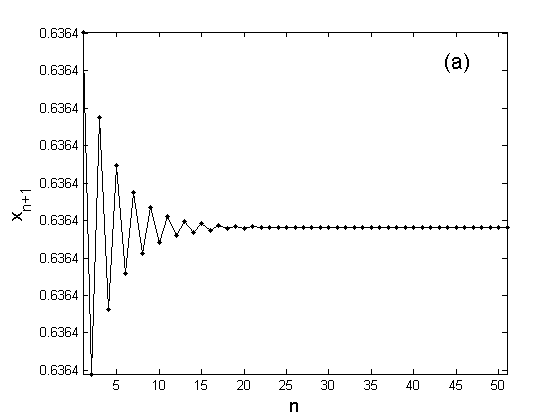
\includegraphics{Figuras/logistico1.png}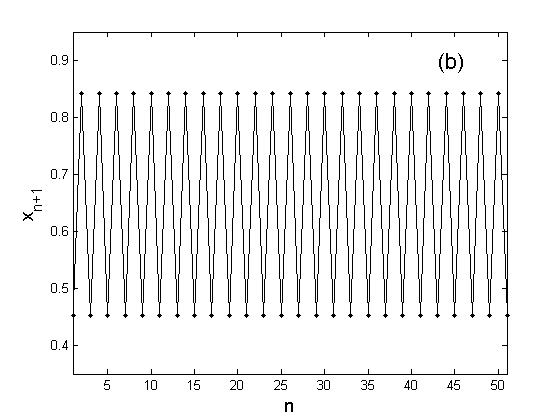
\includegraphics{Figuras/logistico2.png}}\\ \resizebox{15cm}{!}{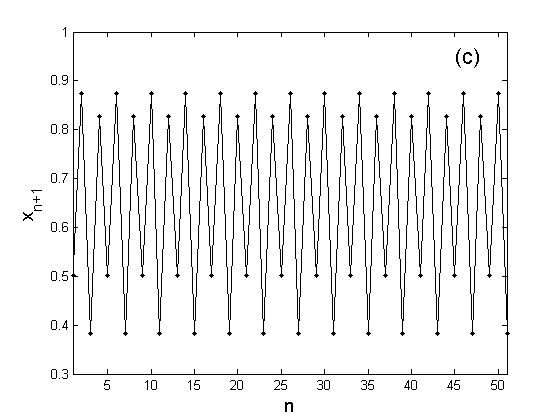
\includegraphics{Figuras/logistico3.png} 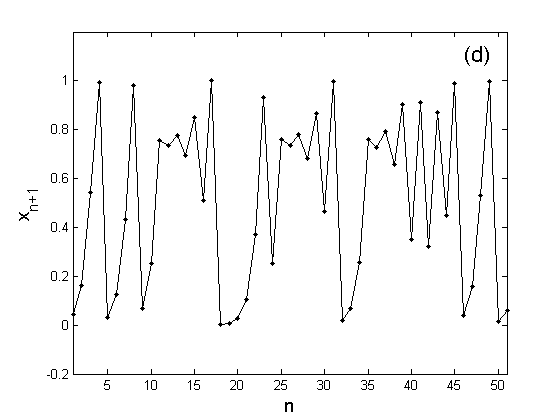
\includegraphics{Figuras/logistico4.png}}
%\caption{Séries temporais obtidas a partir da iteração do mapa~(\ref{equalogis1}) com condição inicial fixa $x_{0}=0.01$ e para valores de $\lambda$ dados, respectivamente por $2.75$, $3.4$, $3.5$ e $4.0$.}
%\label{figuralogis}
%\end{figure}
%
%O mapa logístico também evidencia outra característica dos sistemas caóticos: a \textit{imprevisibilidade}, ou seja, o conhecimento do valor aproximado do estado do sistema não permite predizer, de maneira imediata, sua evolução posterior para qualquer tempo futuro. Este comportamento está associado à \textit{sensibilidade às variações nas condições iniciais} e ao fato de não se conseguir obter com precisão infinita o valor real do estado. Para o Sistema~(\ref{equalogis1}) valores muito próximos de uma condição inicial $x_0$ conduzem, após algumas poucas iterações, a órbitas completamente distintas, conforme pode ser observado na Figura~\ref{figuralogis2}.
%
%\begin{figure}[ht]
%\centering
%\resizebox{15cm}{!}{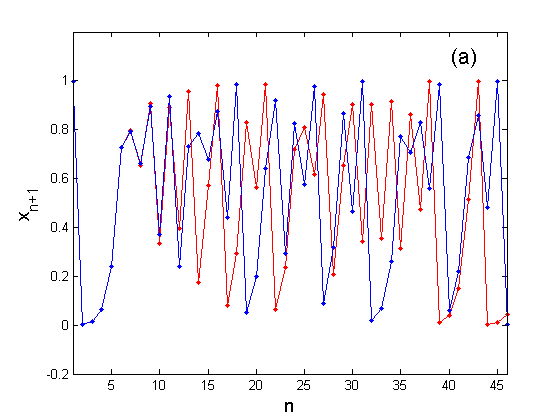
\includegraphics{Figuras/logisticoci.png}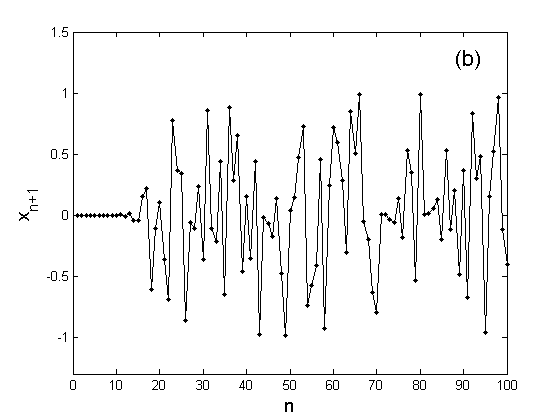
\includegraphics{Figuras/logisticocidiff.png}}
%\caption{(a) Séries temporais obtidas pela iteração do mapa~(\ref{equalogis1}) para valores muito próximos de $x_0$. A curva em azul corresponde à órbita gerada com condição inicial $x_{0}=0.01$, enquanto que a curva em vermelho corresponde à órbita gerada com condição inicial $x_{0}=0.010001$. (b) as diferenças associadas às duas órbitas.}
%\label{figuralogis2}
%\end{figure}
%
%As trajetórias ou órbitas de um sistema caótico oscilam confinados em uma região limitada do espaço de estados, sem entretanto, apresentar periodicidade~\cite{alligood/97}. No interior desta região, as variáveis de estado exibem valores correspondentes a pontos no espaço de fase para os quais as trajetórias caóticas, iniciando em um número significativo de condições iniciais, passam arbitrariamente próximas, infinitas vezes, à medida que o sistema evolui no tempo. Isto é, uma vez iniciada a evolução do sistema, sua trajetória é \textit{atraída} para um sub-conjunto de pontos do espaço de fase, conhecido como \textit{atrator caótico}, e ali permanece percorrendo este sub-conjunto indefinidamente. O conjunto de todas as condições iniciais que converge para o atrator caótico é chamado \textit{bacia de atração} do atrator~\cite{alligood/97}.
%
%Se a estrutura geométrica criada por estados assintóticos das trajetórias for um fractal, este é denominado atrator estranho. Atratores caóticos apenas ocorrem em sistemas dissipativos. Sobre este atrator, a dinâmica é caracterizada por \textit{esticamentos} e \textit{dobras}; o primeiro fenômeno é responsável pela divergência de trajetórias próximas e o último é responsável pela contração da dinâmica para uma região finita em um subespaço de dimensão $\leq m$.  Em contraste com sistemas não-caóticos que possuem atratores de dimensão inteira como pontos atrativos (que geram soluções estacionárias) e ciclos limites (que produzem soluções periódicas), sistemas caóticos podem estar associados a atratores caóticos caracterizados por uma dimensão não-inteira $d$. Esta dimensão é uma propriedade do atrator, independentemente de uma trajetória em particular.
%
%Segundo \citeonline{ruelle/91} atratores caóticos que apresentam o fenômeno da \textit{sensibilidade às variações nas condições iniciais}, correspondem à excitação de um número finito de graus de liberdade e embora tais atratores possuam dimensão finita, a análise em termos de freqüências temporais revela um \textit{espectro contínuo de freqüências}. 
%
%O mapa de Hénon é um exemplo de sistema dinâmico discreto, que apresenta um atrator caótico em sua dinâmica. Este mapa é descrito pelas equações 
%\begin{equation}
%\begin{array}{lcl} x_{n+1} & = & 1-ax_{n}^2+y_{n} \\ 
%                   y_{n+1} & = & bx_{n} \\
%\end{array}
%\label{eqhenon}
%\end{equation}
%sendo $a$ e $b$ parâmetros do mapa. Para valores de $a=1.4$ e $b=0.3$, este sistema apresenta um comportamento irregular e aperiódico que se desenvolve em um atrator caótico e estranho. O atrator de Hénon e uma seqüência de sua ampliação são mostrados na Figura~\ref{figurahenonsimilar}. A dimensão fractal~\cite{mandelbrot/82} associada a esse atrator é de $1.265$, sendo evidente seu caráter auto-similar - característica típica de atratores estranhos~\cite{alligood/97}.
%
%\begin{figure}[ht]
%\centering
%\resizebox{15cm}{!}{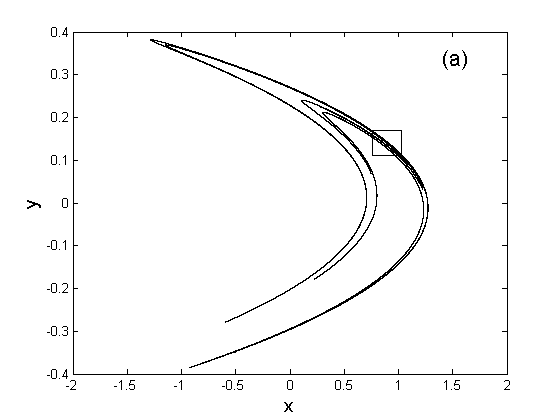
\includegraphics{Figuras/henon.png}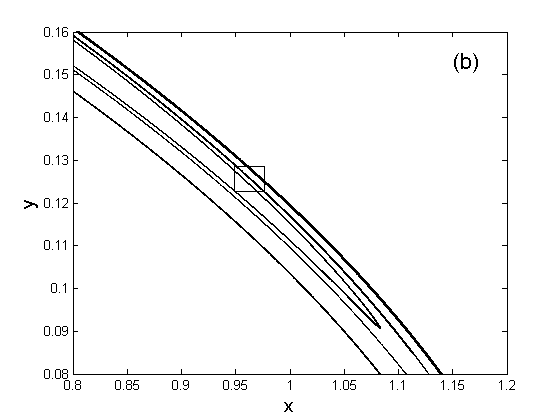
\includegraphics{Figuras/henonamp1.png}}\\ \resizebox{15cm}{!}{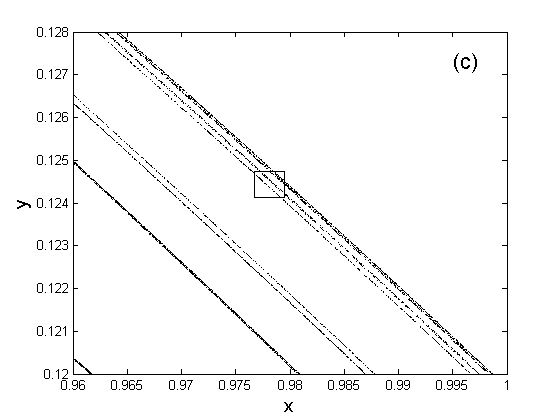
\includegraphics{Figuras/henonamp2.png} 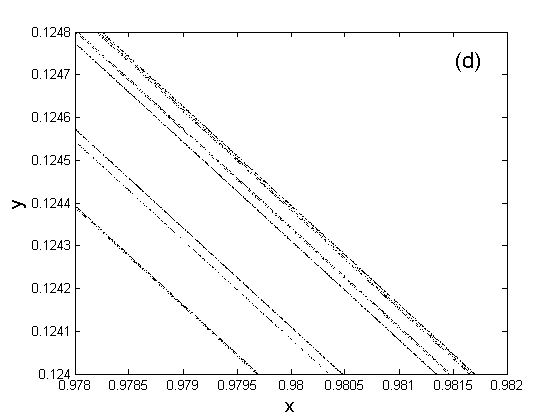
\includegraphics{Figuras/henonamp3.png}}
%\caption{Autosimilaridade do atrator de Hénon. Os pequenos quadrados indicam as regiões de ampliação. (a) $10^3$ iterações. (b) $10^5$ iterações. (c) $10^6$ iterações. (d) $10^7$ iterações.}
%\label{figurahenonsimilar}
%\end{figure}
%
%Para medir a taxa de divergência de trajetórias e, portanto, quantificar a sensibilidade às variações nas condições iniciais, utilizam-se os \textit{expoentes característicos de Lyapunov}. Essa caracterização constitui um dos principais critérios para definir comportamento caótico em sistemas dinâmicos.  
%
%Os expoentes de Lyapunov contêm informações sobre a taxa média com que as trajetórias exponencialmente divergem ou convergem dentro do atrator. Eles estão relacionados às direções de expansão ou contração no espaço de fase~\cite{wolf/85}. Um sistema caótico é caracterizado por uma divergência exponencial de condições iniciais próximas, o que implica em pelo menos um expoente de Lyapunov estritamente positivo. A magnitude do maior expoente positivo (caso exista) reflete a escala temporal sobre a qual o sistema dinâmico torna-se imprevisível~\cite{jaramillo/93}. 
%
%A estimativa dos expoentes de Lyapunov de um sistema dinâmico dissipativo $m$-dimensional requer que se acompanhe a evolução de uma esfera infinitesimal $m$-dimensional de condições iniciais. Com o passar do tempo, a esfera evolui para a forma de um elipsóide. Os expoentes de Lyapunov são definidos tomando o eixo principal do elipsóide. Especificamente, o $i$-ésimo maior expoente $\lambda_{i}$ é definido em termos da taxa de crescimento do $i$-ésimo maior eixo principal, $P_{i}$:
%\begin{equation}
%\lambda_{i}=\lim_{t\rightarrow\ \infty}\frac{1}{t}\log_{2}\left[\frac{P_{i}(t)}{P_{i}(0)}\right]
%\label{eqlyapheuristico}
%\end{equation}
% 
% O conceito de expoente de Lyapunov pode ser apresentado, de forma heurística, considerando uma bola infinitesimal de dimensão $m$ em um espaço de estado. Durante a evolução desse sistema a bola se torna um elipsóide, porém ainda infinitesimal. Denotando o eixo principal deste elipsóide por $\epsilon_{i}(t)\:(i=1,2,\ldots,m)$, os expoentes de Lyapunov $\lambda_{i}$ são determinados por
%  
% \begin{equation}
% \epsilon_{i}(t)\approx\epsilon_{i}(0)e^{\lambda_{i}t}
% \label{eqlyapheuristico}
% \end{equation}
% 
%A soma dos expoentes $\lambda_{i}$, que descrevem a contração do volume, deve ser negativa já que o sistema dinâmico é dissipativo. Desta forma, se um atrator caótico é resultante de esticamentos e dobras, isto requer que pelo menos um dos $\lambda_{i}$ seja positivo. Inversamente, um expoente de Lyapunov positivo implica sensibilidade às variações nas condições iniciais, e desta forma comportamento caótico~\cite{grassbergerstratt/83}.
%
%A Figura~\ref{fighenonlyapunov} apresenta a evolução ao longo do tempo dos expoentes de Lyapunov associados ao Sistema~(\ref{eqhenon}) com condição inicial $(x_{0},y_{0})=(1,1)$. Pode-se observar que um destes expoentes é positivo e dado por $\lambda_{1}=0.42$. Aproximações para os expoentes de Lyapunov, com condições iniciais diferentes, tendem para o mesmo valor $\lambda_{1}$, já que o Sistema~(\ref{eqhenon}) é ergódico. Esse comportamento parece indicar que o sistema apresenta dinâmica caótica.
%
%\begin{figure}[ht]
%\centering \resizebox{10cm}{!}{\includegraphics{Figuras/henonlyapunov.png}} 
%\centering \resizebox{13cm}{!}{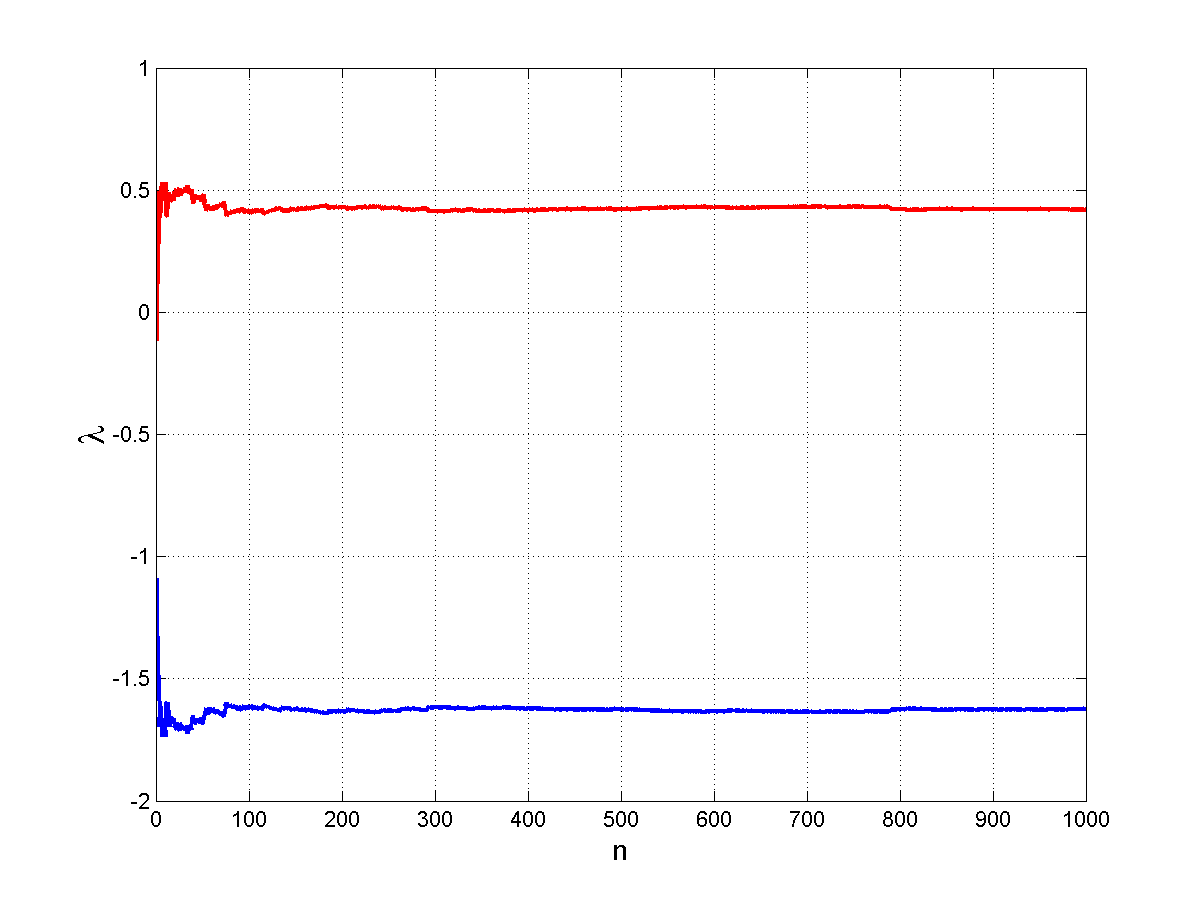
\includegraphics{Figuras/henonlyapunovgrid.png}} 
%\caption{Expoentes de Lyapunov associados ao mapa de Hénon (\ref{eqhenon}) com $a=1.4$ e $b=0.3$.}
%\label{fighenonlyapunov}
%\end{figure}
%
%O artigo clássico de \citeonline{lor/63} foi um dos primeiros trabalhos a descrever movimentos caóticos a partir de um sistema de EDO's, como uma aproximação para a dinâmica de uma camada de fluido convectiva. Suponha que esta camada seja mais quente na base do que no topo (conforme a Figura~\ref{figconveclorenz}), e que a diferença de temperatura $\Delta t$ seja suficiente grande. Sob estas condições o ar mais quente se eleva, deslocando o ar mais frio que está por cima, provocando um movimento convectivo permanente. Se a diferença de temperatura aumentar ainda mais, o escoamento convectivo permanente é perturbado e se instala um movimento turbulento mais complicado~\cite{boyce/99}.
%
%\begin{figure}[ht]
%\centering \resizebox{13cm}{!}{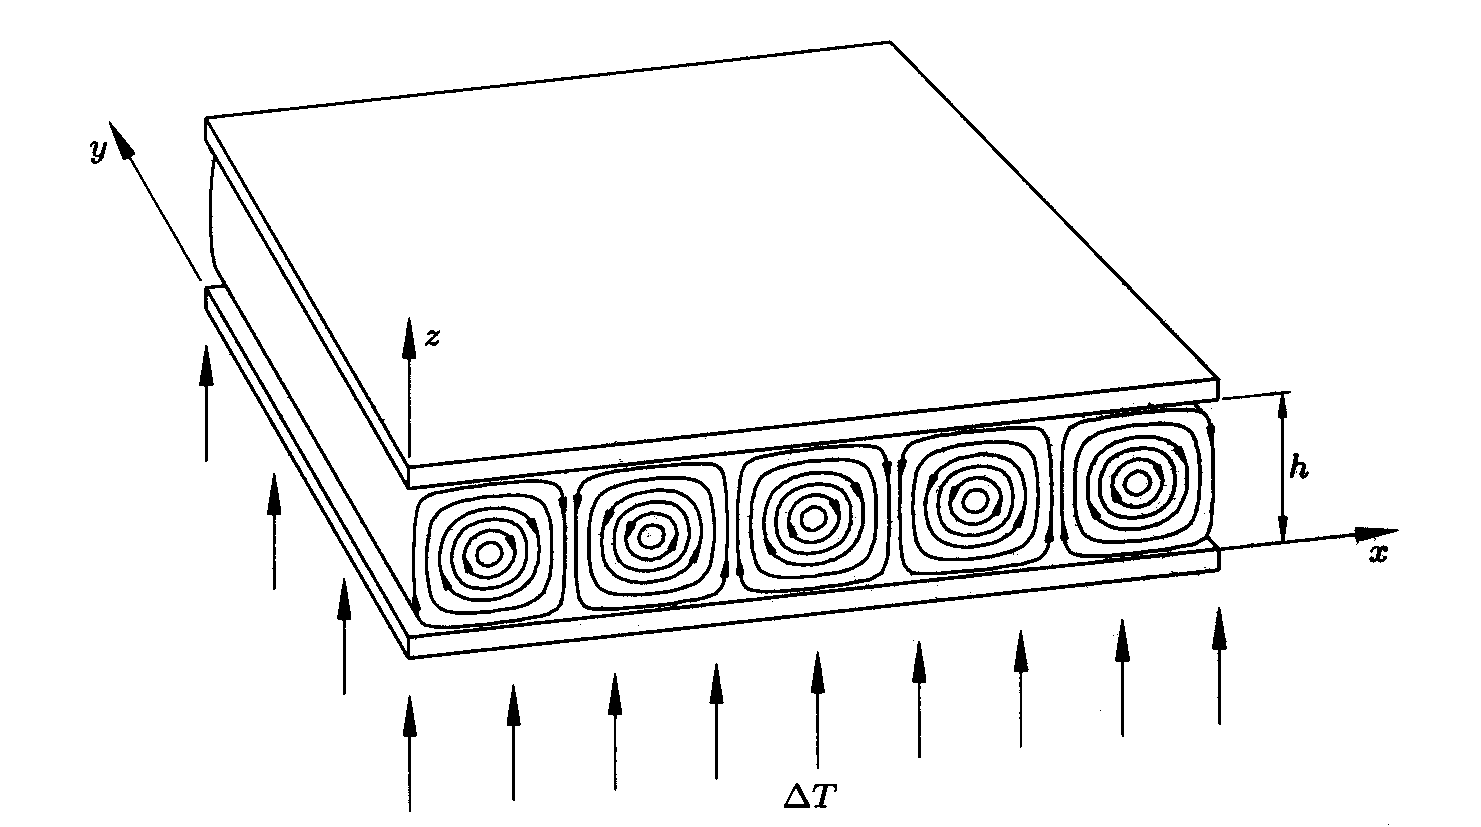
\includegraphics{Figuras/rolo.png}} 
%\caption{Movimento convectivo de uma camada de fluido, com diferença de temperatura $\Delta t$ entre a placa inferior e a superior que o delimita.}
%\FONTE{Adaptada de \citeonline{argyris/94}.}
%\label{figconveclorenz}
%\end{figure}
%
%Ao investigar este fenômeno, Lorenz foi levado, por um processo complexo cuja descrição não é o enfoque deste trabalho, ao sistema autônomo não-linear de EDO's
%\begin{equation}
%\begin{array}{ccc} dx/dt & = & \sigma(-x+y) \\ dy/dt & = & rx-y-xz \\ dz/dt & = & -bz+xy \end{array}
%\label{eqsistemalorenz}
%\end{equation}
%
%As Equações~(\ref{eqsistemalorenz}) são comumente denominadas equações de Lorenz. Pode-se observar que a segunda e a terceira equações envolvem não-linearidades quadráticas. A variável $x$, está relacionada à intensidade do movimento do fluido, enquanto as variáveis $y$ e $z$ estão relacionadas a variações de temperatura nas direções horizontal e vertical. As equações de Lorenz também envolvem três parâmetros $\sigma$, $r$ e $b$, todos reais e positivos. Os parâmetros $\sigma$ e $b$ dependem do material e das propriedades geométricas da camada fluida. No caso da atmosfera, valores razoáveis destes parâmetros são 
%$\sigma=10$ e $b=8/3$~\cite{lor/63}. O parâmetro $r$, por outro lado, é proporcional à diferença de temperatura $\Delta t$, e em todas as simulações posteriores assumirá valor $28$. Desta forma, o Sistema~(\ref{eqsistemalorenz}) assume uma forma particular, dada por
%\begin{equation}
%\begin{array}{ccc} dx/dt & = & 10(-x+y) \\ dy/dt & = & 28x-y-xz \\ dz/dt & = & -8/3z+xy \end{array}
%\label{eqsistemalorenzpart}
%\end{equation}
%
%A Figura~\ref{figlorenzx}(a) apresenta um gráfico de valores calculados de $x$ em função de $t$, ou seja, a evolução no tempo da variável de estado $x$, que é parte da solução do Sistema~(\ref{eqsistemalorenzpart}). Note que a solução oscila entre valores positivos e negativos de uma maneira aparentemente errática. Na realidade, o gráfico de $x$ contra $t$ assemelha-se ao de uma oscilação aleatória, embora as equações de Lorenz sejam inteiramente determinísticas e a solução seja completamente determinada pelas condições iniciais. Não obstante, a solução aparenta, também, uma certa \textit{regularidade}, pois a freqüência e a amplitude das oscilações são essencialmente constantes no tempo.
%
%As soluções das equações de Lorenz são também muito sensíveis a perturbações nas condições iniciais. A Figura~\ref{figlorenzx}(b) mostra os gráficos dos valores calculados de $x$ contra $t$ para duas soluções com condições iniciais bastante próximas. As duas soluções ficam bastante próximas uma da outra, até $t$ nas vizinhanças de $10$, e depois se tornam bastante diferentes, parecendo não ter qualquer relação mútua. Esta propriedade atraiu particularmente a atenção de Lorenz no seu trabalho original sobre as equações, e que tal fato deve estar relacionado à impossibilidade de se ter previsões a longo prazo das condições meteorológicas~\cite{boyce/99}.
%
%\begin{figure}[ht]
%\centering 
%\resizebox{15cm}{!}{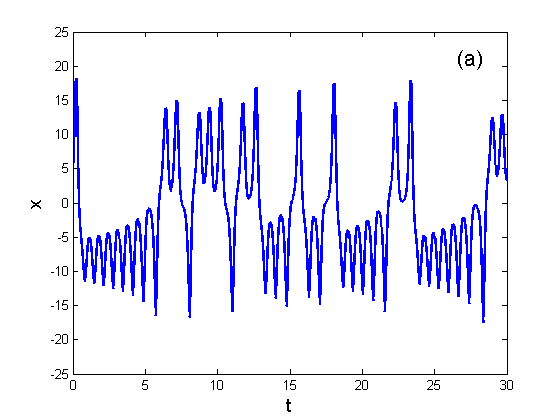
\includegraphics{Figuras/lorenzst.png}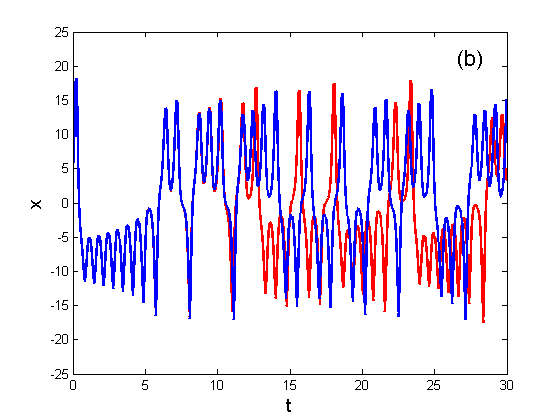
\includegraphics{Figuras/lorenzstci.png}}
%\caption{Séries temporais obtidas a partir da integração do Sistema~(\ref{eqsistemalorenzpart}). (a) condição inicial de $(5,5,5)$. (b) condição inicial da curva em azul é de $(5,5,5)$ enquanto que a da curva em vermelho é de $(5.01,5,5)$.}
%\label{figlorenzx}
%\end{figure}
%
%A Figura~\ref{figlorenzatratorproj} apresenta uma trajetória que principia em $(5,5,5)$ no espaço de fase tridimensional, que se desenvolve em um atrator caótico cuja dimensão de capacidade é de aproximadamente $2.16$~\cite{argyris/94}, como também suas projeções nos planos $xy$, $xz$ e $yz$. Pode-se observar que a trajetória sobre o atrator nunca repete o mesmo caminho; contudo, ela está confinada (atraída) em uma região limitada do espaço de fase. Tal trajetória se alterna sobre um dos dois lóbulos, onde cada um deles contém um ponto crítico instável, e este processo é repetido indefinidamente.
%
%\begin{figure}[ht]
%\centering \resizebox{13cm}{!}{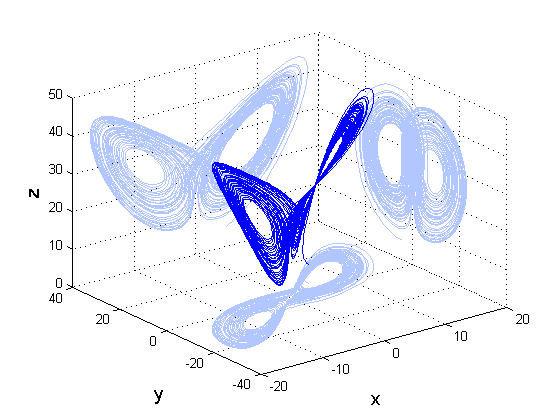
\includegraphics{Figuras/lorenzatratorproj.png} } 
%\caption{O atrator caótico de Lorenz com condição inicial $(5,5,5)$, e suas projeções nos planos $xy$ e $xz$ e $yz$.}
%\label{figlorenzatratorproj}
%\end{figure}
%
%Segundo \citeonline{wolf/85} os expoentes de Lyapunov associados ao Sistema~(\ref{eqsistemalorenz}) (com $\sigma=16$ e $b=4.0$ e $r=45.92$) são dados por
%$\lambda_{1}=2.16$, $\lambda_{2}=0$ e $\lambda_{3}=-32.4$. Desta forma, a dinâmica caótica presente nesse sistema parece se confirmar pela presença de um expoente de Lyapunov positivo~\cite{wolf/85}.
%
%Quando as equações que governam um sistema dinâmico são conhecidas, o estudo das características de suas soluções e de seus invariantes podem revelar comportamentos complexos e interessantes. Porém, em situações reais raramente se dispõe de um conjunto de equações diferenciais ou mesmo um mapa que descreva o comportamento do sistema. Em geral, monitora-se uma única variável, a partir de um experimento que se sabe de antemão depender de outras variáveis. Desta forma, obtém-se uma série temporal de medidas semelhantes às exibidas pelas Figuras~(\ref{figlorenzx}) ou (\ref{figuralogis}) (admitindo-se o não-conhecimento de suas equações) e não se tem acesso às outras variáveis relevantes. A análise de séries temporais com base na teoria de sistemas dinâmicos é um dos temas centrais do Capítulo~\ref{caputiltecnicas}.
%
% 
%\section{Turbulência}
%\label{secturb}
%
%\subsection{Introdução}
%
%O primeiro esboço de um fluxo turbulento, com diversos graus de realismo, foi feito por Leonardo da Vinci no século XV (conforme Figura~\ref{figleonardo}). Para ele o movimento da água em ``redemoinhos'' era devido em parte à sua corrente principal, como também por movimentos contrários e aleatórios. Da Vinci nomeou tal fenômeno de ``la turbolenza''~\cite{richter/70}. 
%
%\begin{figure}[ht]
%\centering \resizebox{13cm}{!}{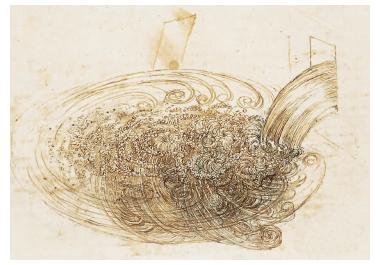
\includegraphics{Figuras/DaVinci3.png}}
%\centering \resizebox{10cm}{!}{\includegraphics{Figuras/DaVincipb.png}} opcao preto e branco!!!
%\caption{Ilustração de Leonardo da Vinci de um fluxo em redemoinhos.}
%\FONTE{\citeonline{ecke/05}}
%\label{figleonardo}
%\end{figure}
%
%Dois aspectos das observações de Leonardo da Vinci têm permanecido até os dias de hoje. Primeiro, a separação do fluxo em uma parte média e outra flutuante, que antecipou em quase $400$ anos a aproximação feita por Osborne Reynolds. Segundo, a identificação de ``vórtices'' como elementos intrínsecos no movimento turbulento. O termo ``vórtice'', usado aqui, refere-se a vários tipos de estruturas turbulentas presentes no escoamento, associadas, por exemplo, ao campo de velocidade de um fluido~\cite{ecke/05}.
%
%\subsection{As equações de Navier Stokes}
%
%Após as descrições feitas por Leonardo da Vinci, o maior avanço na análise do movimento de um fluido foi por meio de equações dinâmicas, como as equações de Navier Stokes (escritas durante o século XIX), que descrevem a taxa de variação da quantidade de movimento em cada ponto de um fluido viscoso. Para um fluido com densidade constante $\rho$ e viscosidade cinemática constante $\nu$, as equações de Navier-Stokes assumem a forma 
%
%\begin{equation}
%\frac{\partial u}{\partial t}+u\cdot\bigtriangledown u=-\frac{\bigtriangledown P}{\rho}+\nu\bigtriangledown ^2u
%\label{eqns1}
%\end{equation}
%
%\begin{equation}
%\bigtriangledown\cdot u=0
%\label{eqns2}
%\end{equation}
%
%Essas equações modelam o escoamento de fluidos incompressíveis, laminares e turbulentos, a partir de condições convenientes impostas nos contornos do fluido. A Equação~(\ref{eqns2}) é a condição de continuidade (sem fontes nem sumidouros), a variável $u(x,t)$ é o campo de velocidade do fluido (incompressível), e $P(x,t)$ é o campo de pressão determinado pela preservação da incompressibilidade~\cite{ecke/05}. O termo $\nu\bigtriangledown ^2u$ representa a contribuição das forças dissipativas lineares da Equação~(\ref{eqns1}), enquanto o termo $u\cdot\bigtriangledown u$ representa a contribuição das forças de inércia não lineares da mesma equação.
%
%A Figura~(\ref{figvulcao}) apresenta a erupção explosiva do Monte St. Helens em sucessivas ampliações, mostrando estruturas em diversos comprimentos de escala. A grande diferença de velocidade, resultante de forças de cisalhamento aplicadas produzem um fluido fortemente turbulento, um estado que pode ser definido como uma solução das equações de Navier-Stokes cujas características exibem flutuações espacial e temporal~\cite{ecke/05}.
% 
%A Equação~(\ref{eqns1}) (quando multiplicada por $\rho$ fornece força por unidade de volume) é simplesmente a lei de Newton para um fluido: força é igual massa vezes aceleração. O lado esquerdo da mesma é a aceleração do fluido\footnote{A aceleração de um fluido é, por definição, a derivada segunda (no tempo) da trajetória do fluido lagrangiano $x(t)$, que descreve o movimento do fluido que estava inicialmente na posição $x(0)$. A primeira derivada é a velocidade lagrangiana do fluido, $dx(t)/dt$ que está relacionada com a velocidade euleriana do fluido por $dx(t)/dt=u(t,x(t))$. Devido $u$ ser uma função do tempo $t$ e da posição $x(t)$, que é por si mesma função do tempo, a expressão euleriana para a derivada segunda lagrangiana (a aceleração do fluido) é obtida através da regra da cadeia e igual a $du/dt=\partial u/\partial t +u\cdot\bigtriangledown u$.}, e seu lado direito é a soma das forças por unidade de massa sobre uma unidade de volume do fluido.
%
%Acredita-se que as equações de Navier-Stokes contêm toda a informação sobre o escoamento turbulento. Embora o problema físico possa em princípio ser completamente revelado pela solução dessas equações, dadas as condições iniciais e de contorno, há uma grande dificuldade devido à sua natureza não-linear~\cite{welter/06}. Mesmo que fosse possível obter uma solução completa de um escoamento turbulento, onde o campo de velocidades $u(x,t)$ pudesse ser conhecido com exatidão em cada ponto do espaço e a cada instante de tempo, esse tipo de conhecimento seria inaplicável devido à dificuldade de armazenagem e processamento da enorme quantidade de informação. Assim, devido os graus de liberdade envolvidos em um escoamento turbulento serem muito grandes,\footnote{Segundo \citeonline{lulandlif/59}, o número de graus de liberdade em um escoamento turbulento é proporcional a $R_{e}^{9/4}$, onde $R_{e}$ é denominado número de Reynolds.} uma das abordagens mais utilizadas é o tratamento estatístico das quantidades de interesse.
%
%\begin{figure}[ht]
%\centering \resizebox{15cm}{!}{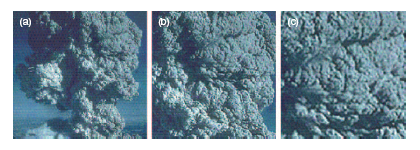
\includegraphics{Figuras/vulcaoturb.png}}
%\caption{(a) A estrutura turbulenta de uma erupção vulcânica do Monte St. Helens, (b) ampliação por um fator de $2$, (c) ampliação por outro fator de $2$. 
%A escala característica da coluna de fumaça é de aproximadamente $5$ Km. }
%\FONTE{\citeonline{ecke/05}}
%\label{figvulcao}
%\end{figure}
%
%
%\subsection {O Número de Reynolds}
%
%Como se sabe, é possível distinguir entre dois tipos de escoamentos. Os escoamentos laminares, que são suaves e determinísticos, e os escoamentos turbulentos, que são abruptos e irregulares no tempo e no espaço. A transição do escoamento laminar para o escoamento turbulento é considerado um dos problemas mais complexos em mecânica dos fluidos. As teorias de transição do escoamento laminar para o turbulento são baseadas nas pequenas perturbações no escoamento. Estas perturbações teriam sua origem nas colisões intermoleculares, e dependendo da estabilidade do escoamento, seriam amplificadas ao passar do tempo e então o escoamento torna-se turbulento~\cite{welter/06}.
%
%Na tentativa de criterizar a transição para a turbulência, \citeonline{reinolds/1895} definiu uma relação entre forças inerciais e viscosas que atuam nos fluidos. Esta razão, um parâmetro adimensional, seria o ponto crítico de transição entre escoamentos laminares e turbulentos. Hoje chamado de \textit{número de Reynolds} ($R_{e}$), este parâmetro é proporcional à razão entre a contribuição das forças inerciais não lineares da Equação~(\ref{eqns1}) e à contribuição das suas forças dissipativas lineares.
%
%Se $U$ é uma velocidade característica do escoamento e $L$ é uma escala de comprimento característico, então as forças inerciais são da ordem de $U^{2}/L$ e as forças viscosas são da ordem de $\nu U/L^{2}$. Assim, o número de Reynolds do escoamento pode ser caracterizado por
%
%\begin{equation}
%R_{e}=\frac{LU}{\nu}
%\label{eqreynolds2}
%\end{equation}
%\newline
%
%Quando o numerador é muito maior que o denominador em~(\ref{eqreynolds2}), o valor de $R_{e}$ é grande e desta forma o fluxo é turbulento, caso contrário o fluxo é laminar (admitindo-se L constante). Em geral, considera-se que o número de Reynolds crítico está entre $2300$ e $3000$. Para números de Reynolds menores que o número de Reynolds crítico, a não-linearidade presente nas equações de Navier Stokes pode ser omitida, e as soluções analíticas para tais equações correspondem a fluxos laminares. Para número de Reynolds maiores que o número de Reynolds crítico não há soluções estacionárias estáveis e o fluido torna-se turbulento. Em particular, o fluxo se encontra na turbulência completamente desenvolvida quando $R_{e}$ é muito maior que aquele obtido na transição para a turbulência, levando-se em conta um conjunto particular de forças e condições de contorno. Na natureza e em laboratórios os escoamentos são em sua maioria turbulentos. Em experimentos laboratoriais em túnel de vento $R_{e}\sim 10^{5}$ e na camada limite atmosférica $R_{e}\sim 10^{7}$~\cite{welter/06}. 
%
%O efeito da variação do número de Reynolds $R_{e}$ em um fluido pode ser vista claramente na Figura~\ref{reynolds1}, que mostra graficamente o padrão de um fluxo uniforme em um cilindro circular. O fluxo, neste caso, é visualizado por uma fumaça ejetada da superfície do cilindro.
%
%Para o estágio (a), $R_{e}\leq 1$, o fluxo é estacionário e não se separa do cilindro. Em (b), $1<R_{e}<10$, o fluxo é ainda estacionário mas um par de vórtices aparecem atrás do cilindro, que aumenta com o incremento de $R_{e}$. Em (c), $10<R_{e}<10^2$, os vórtices estão separados alternativamente do cilindro e alinhados em duas fileiras de vórtices, o conhecido fenômeno dos vórtices de Kármán~\cite{tomomasa/2000}. Neste caso, o fluxo não é mais estacionário e passa a ser periódico.
%
%Em (d), $10^2<R_{e}<10^5$, as fileiras de vórtices tornam-se irregulares e surge um fluxo turbulento, porém ainda laminar fora dele. Em (e), $R_{e}>10^5$, a região torna-se composta de uma grande variedade de vórtices em tamanho e direção, ou seja, o estágio da turbulência completamente desenvolvida. Acima de um certo valor crítico de $R_{e}$, no intervalo $10^5<R_{e}<10^6$, o fluxo no contorno do cilindro também torna-se turbulento.
%
%\begin{figure}[ht]
%\centering \resizebox{9cm}{!}{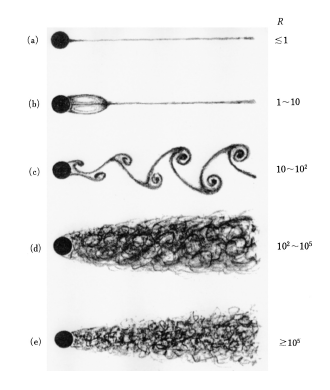
\includegraphics{Figuras/reynoldstomomasa.png}}
%\caption{Mudança no padrão do fluxo de acordo com o número de Reynolds $R_{e}$.}
%\FONTE{\citeonline{tomomasa/2000}}
%\label{reynolds1}
%\end{figure}
%
% As várias simetrias permitidas pela equação de Navier-Stokes são sucessivamente quebradas com o incremento de $R_{e}$, ou seja, quando o fluxo deixa de ser laminar e passa a ser turbulento. Porém, em número de Reynolds ainda mais elevados há uma tendência das simetrias perdidas serem restauradas no senso estatístico, este é o caso da turbulência plenamente desenvolvida, mencionada anteriormente. 
%
%\subsection{Caracterização clássica da turbulência}
%
%\citeonline{lumpano/64} apontam algumas propriedades de um campo turbulento, a saber
%\begin{itemize}
%\item Turbulência é rotacional e dissipativa, isto é, energia mecânica é transformada em calor;
%\item Turbulência é tridimensional; 
%\item Turbulência é não-linear. Todas as escalas estão acopladas entre si no tempo e no espaço;
%\item Turbulência é estocástica. Na prática não importa com qual cuidado as condições de um experimento sejam reproduzidas, o campo de velocidades não poderá ser predito em detalhes; 
%\item Turbulência é um fenômeno contínuo;
%\item Turbulência é difusiva. Um ponto marcado em um fluido turbulento irá vaguear, excursionando para longe de sua posição inicial. Este comportamento é responsável pelo transporte de quantidades (massa, momentum e calor).
%\end{itemize}
%
%O caráter estocástico da turbulência foi questionado por \citeonline{ruelltak/71}. Tais autores introduziram uma interpretação alternativa dos processos turbulentos com base na teoria de sistemas dinâmicos, mais especificamente via ``atratores caóticos de baixa dimensão''. Este assunto será tratado em detalhes na Seção~(\ref{seccaosurb}).
%
%A Figura~\ref{figvelocidadevert} apresenta a evolução de uma variável turbulenta ao longo do tempo, amostrada à $60$Hz. Pode-se observar, que mesmo à uma taxa de amostragem alta, não é possível observar uma variação suave de tal variável com o tempo. O mesmo comportamento é esperado com respeito ao espaço.
%
%\begin{figure}[ht]
%\centering \resizebox{13cm}{!}{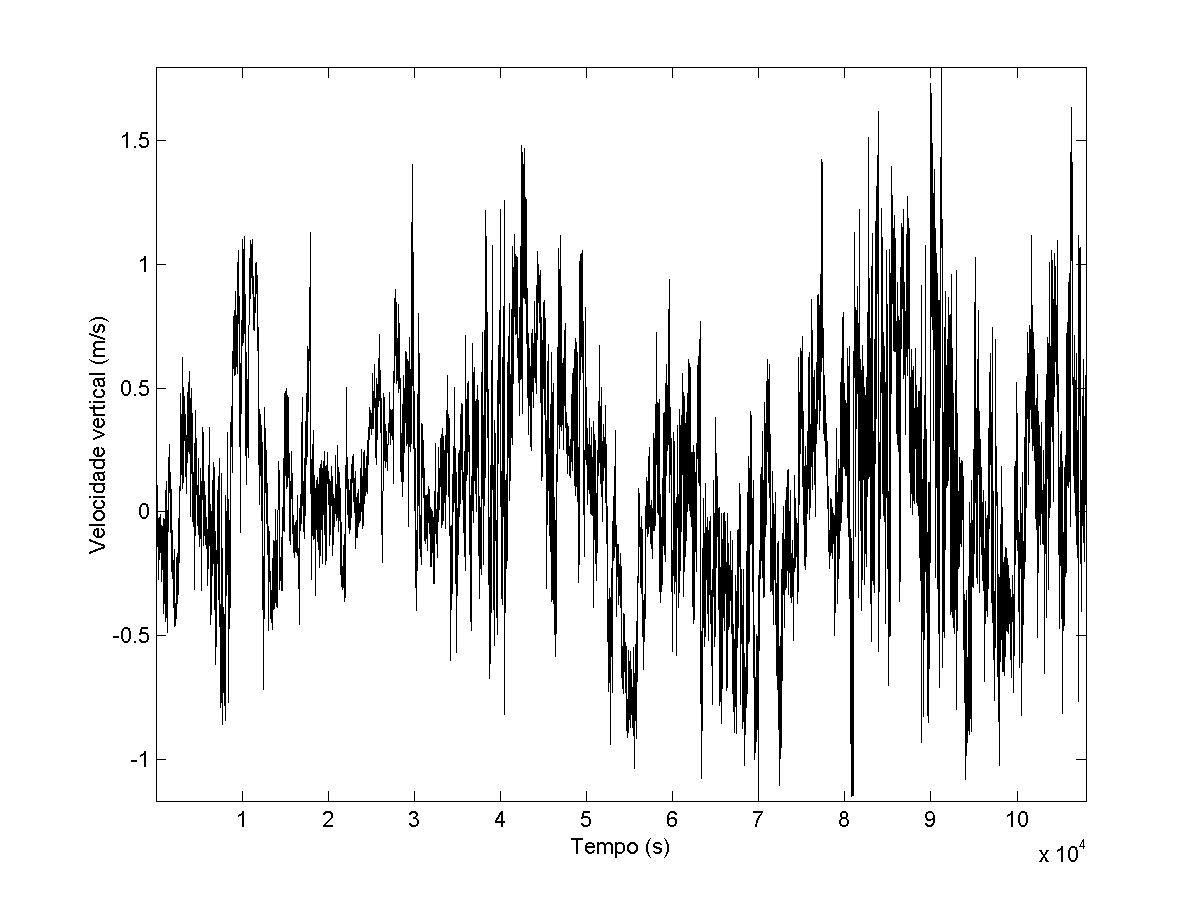
\includegraphics{Figuras/velocidadevert.png}}
%\caption{Evolução temporal de uma variável turbulenta amostrada à $60$Hz.}
%\label{figvelocidadevert}
%\end{figure}
%
%Pode-se imaginar, entretanto, que uma variável turbulenta, como a da Figura~\ref{figvelocidadevert}, é uma composição de um número muito grande de harmônicos e, desta forma, pode-se pensar que a turbulência é composta de uma superposição de vários harmônicos acoplados entre si não linearmente. Estes harmônicos podem ser denominados vórtices. Seguindo esta idéia, um campo turbulento é composto de uma superposição de um número muito grande de vórtices com vários números de onda. Naturalmente, surge a necessidade de se conhecer a distribuição da energia cinética entre estes números de onda~\cite{welter/06}. 
%
%Segundo \citeonline{arya/88}, em escoamentos com elevado número de Reynolds a \textit{Energia Cinética Turbulenta} (ECT) é fornecida aos vórtices nas maiores escalas turbulentas (da ordem de $10^3$m) e, então, dissipada pelos vórtices nas menores escalas (da ordem de $10^{-3}$). A transferência dessa energia ocorre, possivelmente, por meio de um processo de cascata envolvendo todas as escalas intermediárias. Essa idéia foi proposta por Richardson em $1922$~\cite{monin/71} e foi desenvolvida por Kolmogorov em sua teoria sobre turbulência desenvolvida (teoria K41) e, ainda hoje, é objeto de muita discussão~\cite{frisch/96,nelkin/92}. Vórtices maiores colapsam-se em vórtices menores, sucessivamente, até atingirem as menores escalas, onde são destruídos pelas forças viscosas. Desta forma, os vórtices menores não estão diretamente ligados aos processos geradores de energia cinética turbulenta nas maiores escalas (flutuabilidade térmica e cisalhamento vertical da velocidade do vento), permitindo que as escalas intermediárias dessa cascata de energia tenham atributos universais a todos os escoamentos turbulentos. 
%
%A Figura~\ref{espectroesboco} é uma representação esquemática do espectro da ECT. A região $1$ é a de produção de ECT, onde o escoamento médio fornece energia aos maiores vórtices turbulentos através da flutuabilidade e do cisalhamento do vento. Kolmogorov, em $1941$, propôs a \textit{Teoria do Equilíbrio Universal} sobre a similaridade e isotropia da turbulência desenvolvida na pequena escala~\cite{monin/71}. De acordo com essa teoria, para escoamentos com número de Reynolds suficientemente elevados, na Região $2$ da Figura~\ref{espectroesboco}, denominada de \textit{Subdomínio Inercial} (SI), a turbulência é homogênea e isotrópica e nela as propriedades médias do escoamento dependem diretamente apenas de $\epsilon$, a \textit{taxa de dissipação de ECT por unidade de massa}. Ainda, de acordo com a Teoria do Equilíbrio Universal, a região $3$ é onde a ECT transferida pela região $2$ é convertida em calor pela ação da viscosidade, fazendo com que outro parâmetro além de $\epsilon$ seja importante nessa região - a \textit{viscosidade cinemática} $\nu$.
%
%
%\begin{figure}[ht]
%\centering \resizebox{13cm}{!}{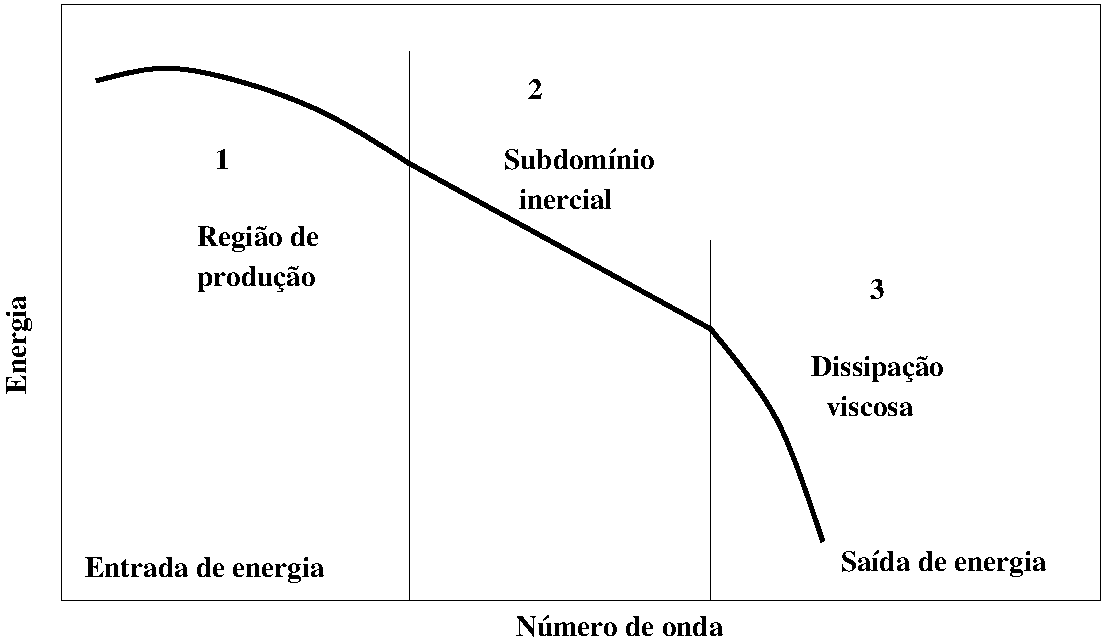
\includegraphics{Figuras/espectroesboco4.pdf}}
%\caption{Representação esquemática do espectro da ECT em escala $\log$-$\log$.}
%\FONTE{Adaptada de \citeonline{garratt/92}}
%\label{espectroesboco}
%\end{figure}
%
% \begin{figure}[!ht]
% \begin{center}
% \resizebox{13cm}{!}{\input{Figuras/espectroesboco5.pdftex_t}}
% \caption{Representação esquemática do espectro da ECT em escala $\log$-$\log$.}
% \FONTE{Adaptada de Garrat~\cite{garratt/92}}
% \label{espectroesboco}
% \end{center}
% \end{figure}
%
%Segundo \citeonline{frisch/96}, no SI o espectro de potência das principais grandezas turbulentas (velocidade, temperatura, umidade, etc) é caracterizado por uma lei de potência com inclinação $-5/3$, ou seja
%
%\begin{equation}
%S_{u}(k)=a k^{-5/3}
%\label{eqespectroturb}
%\end{equation}
%onde $a$ é uma constante de proporçao e $k$ é \textit{o número de onda}. Analogamente, a lei de potência com inclinação $-5/3$ é também obtida para $S_{u}(w)$, onde $w$ é a freqüência.
%
%\subsubsection{Estruturas coerentes em turbulência}
%
%As estruturas coerentes têm sido um assunto de grande relevância na pesquisa em turbulência~\cite{oliver/02}. Este interesse foi intensificado a partir de estudos que demonstraram que a presença dessas estruturas pode ser responsável por até $75\%$ dos fluxos turbulentos na camada da superfície atmosférica\footnote{A porção mais inferior da atmosfera, com extensão de aproximadamente $1$ a $2$ Km, é denominada camada limite atmosférica. Esta é a região mais influenciada diretamente por trocas de momento, calor e vapor de água na superfície da Terra.}~\cite{gao/89}, ou segundo outros autores por, em média, $40\%$ de todo o calor turbulento e fluxos de momento \cite{lu/94,oliver/02}.
%
%Não há uma definição precisa do que sejam estruturas coerentes. Segundo \citeonline{robinson/91} estruturas coerentes de grande escala constituem uma região do fluido turbulento que possui \textit{vorticidade}\footnote{O campo de vorticidade dado por $\omega (x,t)=\bigtriangledown \times u(x,t)$ é uma importante quantidade na caracterização e compreensão do fluxo turbulento. De forma geral, ele mede a rotação de um fluxo. Na turbulência 3-D, a vorticidade desempenha uma função quantitativa na qual a taxa média de energia dissipada $\varepsilon$ está relacionada com o quadrado da vorticidade pela relação $\varepsilon=-u\langle|\omega|^2\rangle$~\cite{ecke/05}.}\textit{coerente} sobre uma significativa extensão espacial. Essas estruturas podem ainda ser caracterizadas por uma região tridimensional, onde pelo menos uma das variáveis fundamentais do escoamento (componente de velocidade, massa específica, temperatura, etc.) apresenta significativa correlação com ela mesma ou com outra variável, num intervalo de espaço e/ou tempo suficientemente maior que as menores escalas locais do escoamento.
%
%As estruturas coerentes são características da turbulência de grande escala na camada da superfície atmosférica. Sob condições convectivas instáveis, elas são reconhecidas em séries temporais de flutuações de temperatura com uma gradual elevação da temperatura, seguida por uma súbita queda. Sob condições estáveis, este padrão se inverte e uma gradual queda é seguida por uma súbita elevação~\cite{oliver/02}. Nestas duas condições, a estrutura coerente é do tipo ``rampa''. 
%
%O efeito das condições de estabilidade sobre o comportamento em rampa das estruturas coerentes é uma conseqüência direta da distribuição espacial de fontes de calor e umidade. Por exemplo, durante o dia o ar aquecido está localizado próximo à superfície, assim a súbita queda de temperatura é devido à presença do ar mais frio que se desloca para baixo e, durante a noite, a súbita elevação da temperatura está associada com o ar mais quente que se desloca para baixo. Desde que a fonte de umidade esteja situada apenas na superfície, as estruturas coerentes presentes em séries temporais de flutuações de umidade mostram um padrão independente de estabilidade.
%
%\subsubsection{Intermitência em turbulência}
%
%A intermitência é um fenômeno relacionado à presença de raros, porém fortes gradientes de velocidade com acentuada localização no espaço ou no tempo. Esses gradientes são gerados por estruturas altamente coerentes (quase sempre não estacionárias) e são responsáveis pelo forte aumento da taxa de dissipação local da ECT~\cite{camussi/97}.
%
%Segundo \citeonline{frisch/96} uma função aleatória é intermitente se o quarto momento estatístico normalizado, a saber, a curtose definida como
%\begin{equation}
%K(r)=\frac{\langle u_{r}^4\rangle}{{\langle u_{r}^2\rangle}^2}
%\label{eqintermitencia}
%\end{equation}
%cresce sem limites quando $r\rightarrow 0$. Desta forma, pode-se afirmar que a curtose é uma grandeza estatística que quantifica a presença de fenômenos intermitentes em um escoamento turbulento, sendo um parâmetro que mede o grau de achatamento de uma \textit{Função de Distribuição de Probabilidade} (FDP). 
%
%A presença da intermitência em um sinal turbulento confere uma forma especial à sua FDP. Para o caso da turbulência atmosférica, as FDP's são, em geral, aproximadamente gaussianas nas maiores escalas do escoamento (com valores de curtose próximos de $3$) e fortemente não gaussianas em suas menores escalas, devido ao fenômeno da intermitência. As curvas da Figura~\ref{figpdfintermitente} são histogramas de $\Delta u_{r}=u(x+\Delta r)-u(x)$ obtidos para distâncias de separação (usando a hipótese de Taylor $\Delta r=U\Delta t$) dadas por $\Delta r=4,40,400$ e $4000$. Para dados amostrados a $60$ Hz essas distâncias correspondem a $\Delta t$ de $0.06,0.66,6.66,66.66$ segundos, respectivamente. Nas menores escalas de separação, ocorrem grandes flutuações com uma freqüência muito maior que aquela prevista para um processo gaussiano. Este fenômeno, diretamente ligado à intermitência do escoamento turbulento, aparece nas FDP's sob a forma de ``asas'' ou ``caudas'' prolongadas.
%Fernando
%
%\begin{figure}[ht]
%\centering \resizebox{13cm}{!}{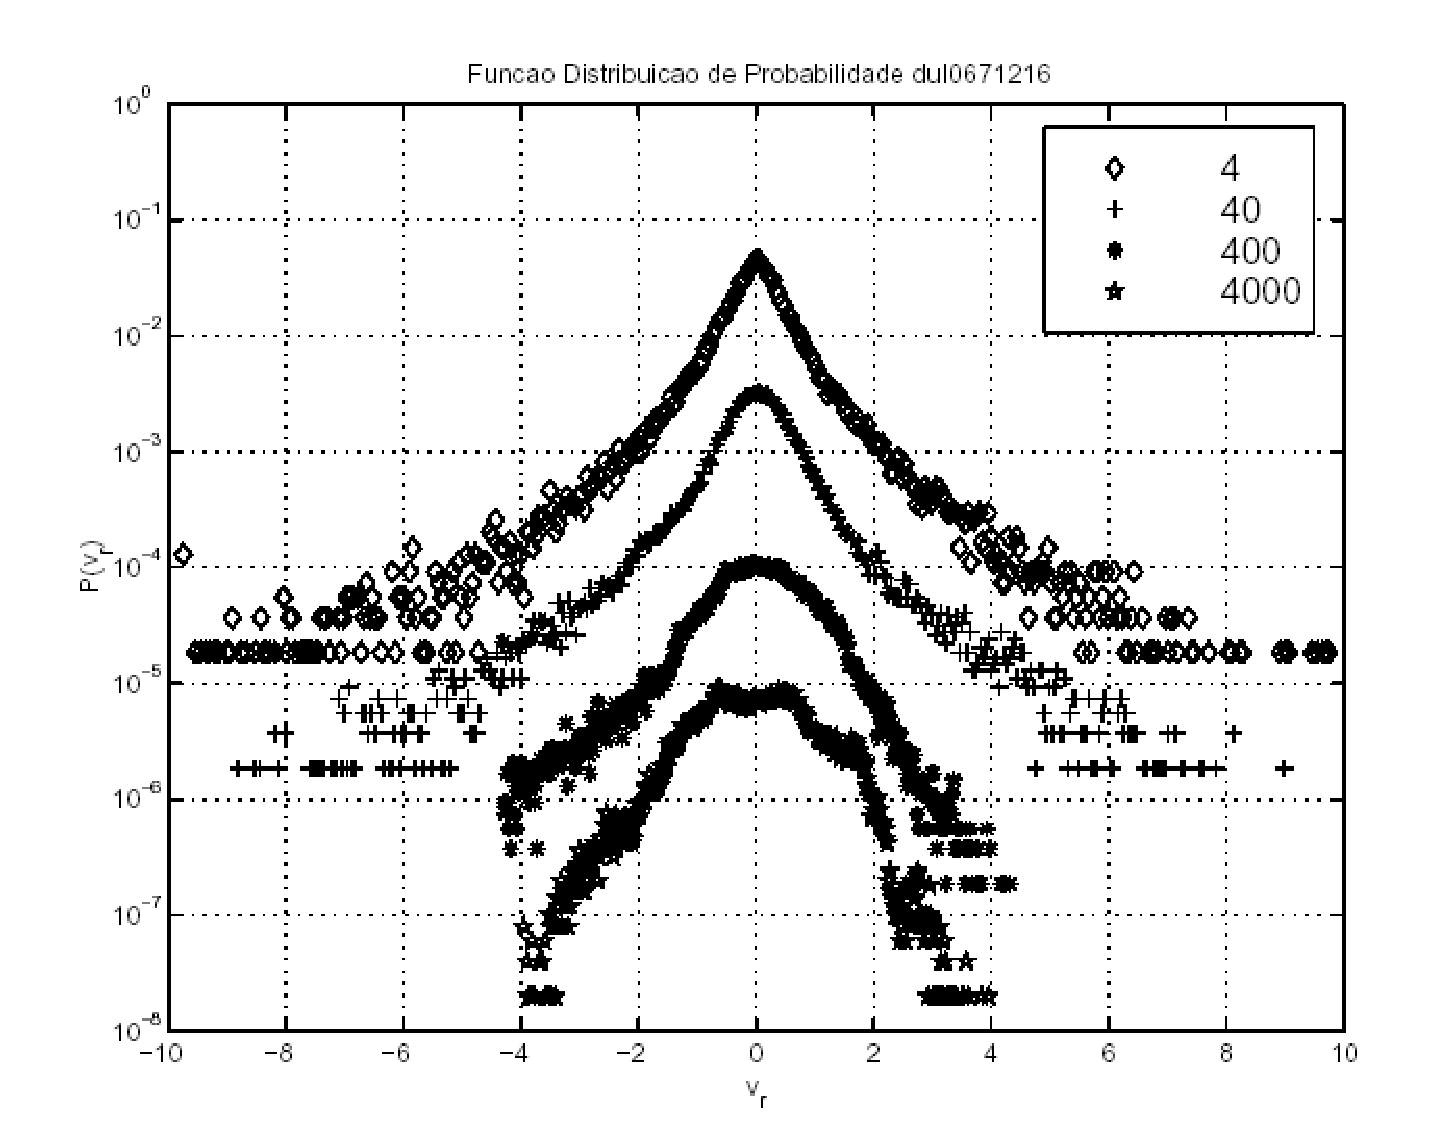
\includegraphics{Figuras/bolzan.pdf}}
%\caption{PDF's das diferenças de velocidade longitudinal dentro da copa da Floresta Amazônica, para valores de $\Delta r=4,40,400$ e $4000$.}
%\FONTE{\citeonline{bolzan/00}}
%\label{figpdfintermitente}
%\end{figure}
%
%\section{Caos e Turbulência}
%\label{seccaosurb}
%
%O desenvolvimento da teoria de sistemas dinâmicos caóticos, tem fornecido importantes subsídios à compreensão do fenômeno da turbulência. Uma conjectura feita por Landau foi a primeira tentativa para a descrição do surgimento da turbulência. Conforme sua teoria, o comportamento turbulento é causado por uma seqüência infinita de bifurcações de Hopf. Desta forma, cada vez que uma bifurcação ocorre, freqüências fundamentais\footnote{A cada nova freqüência associa-se um novo grau de liberdade ao sistema} são adicionadas ao sistema e a medida que cada vez mais freqüências ocorrem, o movimento torna-se cada vez mais turbulento~\cite{grebogi/83}. 
%
%A idéia defendida por Landau, de que um fenômeno complexo tal como a turbulência necessite de uma descrição complexa com infinitos graus de liberdade, foi contestada a partir do estudo de Lorenz que mostrou que um sistema com apenas três EDO's pode levar a comportamentos complexos e caóticos~\cite{argyris/94}. A concepção de Landau foi ainda fortemente questionada for \citeonline{ruelle/91}, sobretudo pela ausência tanto da sensibilidade às variações nas condições iniciais quanto de espectros contínuos em sua conjectura.
%
%O trabalho pioneiro de \citeonline{ruelltak/71} introduziu uma nova e promissora perspectiva para a compreensão do fenômeno turbulento. Esses autores foram os primeiros estudiosos a propor um possível mecanismo de transição de um fluxo laminar para um fluxo turbulento com base na teoria de sistemas dinâmicos, mais especificamente por meio de atratores caóticos. Com base nessa abordagem Ruelle, Takens, Feigenbaum, e outros autores, investigaram ``rotas para a turbulência'', ou seja, cenários (sucessões de bifurcações) nos quais um sistema com uma evolução temporal simples torna-se turbulento quando um ou mais de seus parâmetros são alterados~\cite{ruellelecture/90}.  
%
%\subsection{Bifurcação e rotas para a turbulência}
%
%
%O \textit{cenário Ruelle-Takens}~\cite{ruelltak/71} propõe uma rota baseada em três bifurcações consecutivas: ponto fixo $\longrightarrow$ ciclo limite $\longrightarrow$ toro\footnote{O toro $k$-dimensional $T^{k}$ pode ser entendido como o produto de $k$ círculos} $T^{3}$ $\longrightarrow$ atrator caótico (turbulência). Em outras palavras, movimentos quasiperiódicos sobre um toro $T^{3}$ (ou seja, com três freqüências incomensuráveis) podem perder estabilidade e surgir diretamente a turbulência~\cite{zeng/93,newhouse/78}. Esta rota é genérica e ocorre em diversos modelos matemáticos e em experimentos de laboratório, porém ela é uma rota de difícil compreensão teórica que as demais rotas mencionadas abaixo~\cite{zeng/93}.
%
%\citeonline{eckmann/81} propôs outra rota para a turbulência, que é conhecida como rota para a turbulência de Feigenbaum ou de duplicação de período: uma cascata de bifurcações de duplicações de período $p = 2^{n}(n=0,1,2,\ldots)$ que converge rapidamente para uma órbita aperiódica quando $n\rightarrow \infty$. Este cenário tem sido validado com grande êxito em diversas simulações numéricas e sistemas físicos. A duplicação de período tem sido observada em experimentos como a convecção de Rayleigh-Bénard~\cite{zeng/93}.
%
%A quarta rota, chamada de rota para a turbulência de Pomeau-Manneville, é através da intermitência~\cite{pomeau/80}. No contexto de sistemas caóticos, o termo \textit{intermitente} refere-se a alterações aleatórias entre um comportamento caótico e regular no tempo sem envolver nenhum grau de liberdade espacial. Este conceito é diferente do significado original da \textit{intermitência} na teoria hidrodinâmica da turbulência, que indica ``estouros'' aleatórios do movimento turbulento sobre a base de um fluxo laminar~\cite{zeng/93}. Nesta rota não há uma clara compreensão de quando o regime turbulento é alcançado nem da exata natureza desta turbulência~\cite{eckmann/81}. 
%
% Especificamente, pode-se afirmar que a rota Ruelle-Takens está relacionada a bifurcações do tipo Hopf, onde um par de autovalores complexos cruza o círculo unitário; a rota de Feigenbaum está associada com bifurcações do tipo Pitchfork, onde um autovalor cruza o círculo unitário em $-1$; e a rota Pomeau-Manneville está associada com bifurcações do tipo Sela-Nó, onde um autovalor cruza o círculo unitário em $1$. 
%
%
%A Tabela~\ref{tabbifurca} apresenta a evolução da dinâmica de um sistema, de um estado estacionário à um estado turbulento, sob a influência de diferentes sucessões de bifurcações.
%
%\begin{sidewaystable}
%\caption{Rotas para a turbulência com base em seqüências de bifurcações}
%\vspace{0.5cm}
%\begin{center}
%\resizebox{!}{3.6cm}{
%\begin{tabular}{c c c c c c c c c c c c}
%\hline 
%\multicolumn{1}{c}{\textbf{}} & \multicolumn{11}{c}{\textbf{}} \\
%\multicolumn{1}{c}{\textbf{Rotas}} & \multicolumn{11}{c}{\textbf{Seqüências de bifurcações}}\\
%\multicolumn{1}{c}{\textbf{}} & \multicolumn{11}{c}{\textbf{}}\\
%\cline{1-12}
%\hline 
%\textbf{} & Ponto & $\longrightarrow$ & Órbita & $\longrightarrow$ & Órbita & $\longrightarrow$ & Órbita & $\longrightarrow$ & $\cdots$ & $\longrightarrow$ & Movimento \\
%\textbf{Landau} & estacionário & (Hopf) & periódica & (Hopf) & periódica & (Hopf) & periódica & & (Hopf) & & turbulento \\
%\textbf{} & & & única &  & dupla &  & tripla & & & &  \\
%& & &  &  &  &  &  & & & &  \\
%\hline
%\textbf{Ruelle-} & Ponto & $\longrightarrow$ & Órbita & $\longrightarrow$ & Órbita & $\longrightarrow$ & Atrator &  &  & & \\
%\textbf{Takens} & estacionário & (Hopf) & periódica & (Hopf) & periódica & (Hopf) & caótico &  &  & &  \\
%\textbf{} & &  & única &  & tripla &  &  &  &  & & \\
%& & &  &  &  &  &  & & & &  \\
%\hline
%\textbf{} & Ponto & $\longrightarrow$ & Órbita & $\longrightarrow$ & Órbita & $\longrightarrow$ & Órbita & $\longrightarrow$ & $\cdots$ & $\longrightarrow$ & Atrator \\
%\textbf{Feigenbaum} & estacionário & (Hopf) & periódica & (Duplicação & periódica & (Duplicação & periódica &  & (Duplicação &  & Caótico \\
%\textbf{} & & & única & de & única & de & única &  & de &  &  \\
%\textbf{} & & & (período $T$) & período) & (período $2T$) & período) & (período $4T$) &  & período) &  &  \\
%& & &  &  &  &  &  & & & &  \\
%\hline
%\textbf{Pomeau-} & Ponto & $\longrightarrow$ & Órbita & $\longrightarrow$ & Movimento &  &  &  &  &  & \\
%\textbf{Manneville} & estacionário &(Hopf) & periódica &  & caótico &  &  &  &  &  &  \\
%\textbf{} & & & única &  & intermitente &  &  &  &  &  &  \\
%\hline
%\end{tabular}}
%\begin{flushleft}
%\tamfonte: {Adaptada de \cite{miles/84}}
%\end{flushleft}
%\label{tabbifurca}
%\end{center}
%\begin{flushleft}
%\vspace{0.2cm}\hspace{1.6cm}\tamfonte: {Adaptada de \citeonline{miles/84}}
%\end{flushleft}
%\end{sidewaystable}
%
%
%De modo geral, todas as rotas descritas acima, estão relacionadas à turbulência em seu estágio inicial (turbulência fraca), ou seja, quando a mesma pode ainda ser descrita por um número reduzido de graus de liberdade~\cite{chenmin/05}. Segundo \citeonline{zeng/93}, a compreensão do fenômeno turbulento será alcançada quando o mecanismo inicial que lhe deu origem for completamente entendido. Tal idéia justifica, em grande parte, a importância do estudo das rotas para a turbulência. Sob essa perspectiva, a turbulência fraca e caos possuem características em comum, já que ambos apresentam comportamentos irregulares em sua evolução temporal e podem ainda ser descritos por um conjunto reduzido de equações diferenciais determinísticas. Em contrapartida, a turbulência totalmente desenvolvida (com elevados números de Reynolds) envolve irregularidades de caráter temporal e espacial e só pode ser descrita por um número de graus de liberdade elevado.
%
%\subsection{Caracterização da turbulência via atratores caóticos}
%
%Desde que Lorenz introduziu seu modelo inspirado em dinâmica dos fluidos (conforme Seção~\ref{seccaos} deste capítulo), conjectura-se que a atmosfera possui um intrínseco limite de previsibilidade e que a dinâmica atmosférica é governada por um atrator caótico~\cite{weber/95}. 
%
%Diversos trabalhos confirmam a existência de atratores na atmosfera, com base em séries temporais turbulentas. Esses atratores foram detectados, de maneira geral, a partir da técnica da reconstrução de espaço de fase~\cite{tak/81}, que será discutida em detalhes no Capítulo~\ref{caputiltecnicas}. \citeonline{xin/01} detectaram a existência de atratores caóticos, com dimensão de correlação entre $3$ e $7$, a partir de dados turbulentos observados na camada limite atmosférica. Esses dados foram amostrados a $16$ Hz e incluem medidas de temperatura, umidade e velocidade do vento em três direções, obtidos na província de Gansu e em Beijing, China. 
%
% Diversos trabalhos confirmam a existência de atratores de baixa dimensão na atmosfera, com base em séries temporais turbulentas. Esses atratores foram detectados a partir da técnicas como a reconstrução de espaço de fase \ref{eqtakensreconst}, pelo algoritmo de Grassberger e Procaccia \ref{eqcorr1} e ainda pelo algoritmo de Wolf~\cite{wolf/85}. Xin \textit{et al} \cite{xin/01} detectaram a existência de atratores estranhos, com dimensão entre $3$ e $7$, a partir de dados turbulentos observados na camada limite atmosférica. Esses dados foram amostrados a $16$ Hz e incluem medidas de temperatura, umidade e velocidade do vento em três direções, obtidos na província de Gansu e em Beijing, China. 
%
%\citeonline{jaramillo/93} analisaram $24$ séries temporais de velocidade do vento e flutuações de temperatura, amostrados a $10$ Hz, em períodos de $30$ minutos, sobre condições atmosféricas instáveis, e concluiram que atratores caóticos com baixa dimensão, com dimensão de correlação entre $4$ e $6$, governam a dinâmica da baixa atmosfera de Ontário, Canadá. 
%
%A partir de dados de três componentes do vento, medidos em Almaraz (Cáceres, Espanha) à $18$ Hz, \citeonline{gallego/01} identificaram atratores caóticos para a turbulência convectiva com dimensão de correlação de aproximadamente $6$ e para a turbulência mecânica com dimensões de correlação variando entre $7$ e $9$. 
%
%Alguns trabalhos negam a existência de atratores caóticos na atmosfera. Nenhum indício de um atrator foi encontrado nas análises realizadas por \citeonline{weber/95} com base em séries temporais turbulentas das componentes vertical e horizontal da velocidade do vento, amostradas à $21$ Hz. \citeonline{loratrat/91} afirma que não há razão alguma para acreditar que um sistema dinâmico complexo, como o clima, possua um atrator de baixa dimensão associado. Segundo Lorenz, o valor da dimensão de correlação obtido em diversas análises, com base em séries temporais climáticas, pode estar relacionado à dimensão de um conjunto de subsistemas de baixa dimensão ``fracamente'' acoplados~\cite{loratrat/91}, e não à dimensão de um atrator associado ao sistema como um todo. A validade ou não deste cenário será investigada no Capítulo~\ref{caputiltecnicas}. Essa questão acerca da dimensão de um eventual atrator caótico associado à dinâmica da atmosfera está ainda em aberto, aguardando novos experimentos e o desenvolvimento de métodos inovadores de análise de séries temporais.
 %% 2o capítulo

%%%%%%%%%%%%%%%%%%%%%%%%%%%%%%%%%%%%%%%%%%%%%%%%%%%%%%%%%%%%%%%%%%%%%%%%%%%%%%%%
% CAPÍTULO 4

\chapter{ASPECTOS GERAIS DAS TÉCNICAS UTILIZADAS}
\label{caputiltecnicas}

Neste capítulo é feita uma descrição detalhada dos métodos e dos algoritmos disponíveis para a caracterização de caos determinístico presente em séries temporais experimentais. Tal descrição será focada nos procedimentos mais utilizados para a reconstrução da dinâmica, para o cálculo de dimensão de atratores e do espectro de expoentes de Lyapunov. São abordados alguns problemas e limitações, do ponto de vista numérico, associados aos algoritmos utilizados, como também as dificuldades encontradas no tratamento de sinais experimentais. 

\section{Caos em séries temporais}

\subsection{Introdução}

\citeonline{alligood/97} afirmam que ``Obviamente, a idéia de que um experimento real possa ser governado por um conjunto de equações é uma ficção. Um conjunto de equações diferenciais, ou um mapa, pode modelar um sistema apenas de forma o suficiente para fornecer resultados úteis''. Por outro lado, a informação completa de todos os graus de liberdade de um sistema dinâmico complexo na natureza é raramente conhecida em sua totalidade. Por exemplo, em um fluido, esta informação deveria incluir sua velocidade em todas as posições como função do tempo, o que é inviável na prática. Neste contexto, torna-se importante analisar sistemas dinâmicos sem que se conheça detalhes sobre a sua dinâmica interna, ou seja, sistemas que não possuem um modelo matemático estabelecido. Uma alternativa para isso é a análise de séries temporais que podem ser obtidas diretamente a partir de um experimento~\cite{kantz/97}.

De uma maneira geral, em um experimento monitora-se uma única variável do sistema, que se sabe de antemão depender das outras. Ou seja, obtém-se uma série temporal de medidas e, na maioria dos casos, não se tem acesso às outras variáveis relevantes (muitas vezes não se sabe ao certo sequer quantas são) e muito menos se dispõe de um modelo (equações diferenciais ou mapas) que descreva o comportamento do sistema. Caso se soubesse exatamente quais são as variáveis relevantes e as mesmas pudessem ser medidas simultaneamente, poderia ser construído um espaço de fase do sistema e nele representar a dinâmica do sistema~\cite{aguirre/00}.

Nesta seção apresenta-se, de maneira geral, um resumo de diversas técnicas utilizadas na identificação de séries temporais caóticas, discutem-se suas principais limitações e enumeram-se quais informações pode-se extrair de sinais experimentais através desses procedimentos. Sempre que possível, tais técnicas serão validadas a partir de uma série temporal que apresenta comportamento caótico, a saber, a componente $x$ do sistema de Lorenz, que foi obtida a partir da solução numérica do Sistema~(\ref{eqsistemalorenzpart}) pelo método de Runge-Kutta de quarta ordem.

\subsection{A Análise Tradicional de Sinais Experimentais}
\label{secanalisetrad}

A identificação de processos regulares pode ser feita através do uso de métodos clássicos. Incluem-se entre eles: a \textit{análise espectral} (espectro de potências) e a \textit{função de autocorrelação}, os quais serão introduzidos a seguir.

Seja a evolução de um sistema dinâmico dada por uma função $f(t)$, ou, quando resultado de uma série de medidas realizadas a intervalos de tempos regulares $\Delta t$, representada por uma série temporal da forma

\begin{equation}
{x_{n}}=x(t_{n}), \;\;\;\; t_{n}=n\Delta t
\label{eqserietemp}
\end{equation}

Sob condições bem gerais, uma função $f(t)$ pode ser considerada como sendo a superposição de um número (eventualmente infinito) de componentes periódicas. A determinação do peso relativo de cada uma dessas componentes é chamada de \textit{análise espectral}. Se $f(t)$ é periódica, seu espectro pode ser representado como a combinação linear de oscilações cujas freqüências são múltiplos inteiros da freqüência básica $\omega$. Essa combinação linear é chamada \textit{série de Fourier}~\cite{papoulis/62}. Quando $f(t)$ é não-periódica, o espectro de freqüências varia continuamente e usa-se a chamada \textit{transformada de Fourier} para representar $f(t)$ em termos dessas freqüências~\cite{papoulis/62}. Escreve-se a transformada de Fourier de $f(t)$ como
\begin{equation}
f(\omega)=\int_{-\infty}^{+\infty}e^{-i\omega t}f(t)dt
\label{eqfouriercont}
\end{equation} 

O espectro de potências $P(\omega)$, que indica o ``peso relativo'' com que a freqüência $\omega$ comparece na composição de $f(t)$, é definido como o quadrado do módulo de $f(\omega)$, ou seja,
\begin{equation}
P(\omega)=\left|f(\omega)\right|^2
\label{eqespectrocont}
\end{equation} 

Na situação de interesse prático, dispõe-se de uma série temporal finita e discreta da forma~(\ref{eqserietemp}). Se $N$ é o número total de pontos na série, então ${x_{n}}$ corresponde a um tempo total de medida $t_\textrm{max}=N\Delta t$. A transformada discreta de Fourier, de uma série temporal, é definida por uma outra série $\widehat{x}_{k}$ tal que
\begin{equation}
\widehat{x}_{k}=\frac{1}{\sqrt{N}}\sum_{n=1}^{N}x_{n}\exp\left[i\frac{2\pi nk}{N}\right],\;\;\;\;\;\;\;k=1.\ldots,N
\label{eqfourierdis}
\end{equation} 

A série temporal~(\ref{eqserietemp}) depende do tempo; por outro lado, $\widehat{x}_{k}$ depende das freqüências, isto é, $\widehat{x}_{k}=\widehat{x}(\omega=k\Delta f)$ com $\Delta f= 1/t_{\textrm{max}}$. O cálculo da transformada discreta de Fourier (\ref{eqfourierdis}) pode ser feito com rapidez através do uso do algoritmo conhecido como FFT (\textit{Fast Fourier Transform})~\cite{cooleytukey/65}.

O espectro de potências $P(\omega)$ para uma série temporal discreta é definido por
\begin{equation}
P(\omega)=\left|\widehat{x}_{k}\right|^2
\label{eqespectrodiscr}
\end{equation} 

Séries temporais com evoluções diferentes apresentam diferentes espectros de potência. Sinais periódicos de período $T$ apresentam um pico bem definido na freqüência correspondente a esse período. Por outro lado, séries temporais caóticas apresentam espectros de potência com uma ``banda larga'', o que indica a existência de um contínuo de freqüências. Séries aperiódicas sem comportamento caótico também podem apresentar um espectro de potência com uma banda larga, e desta forma, é necessário outras ferramentas para caracterizar comportamento caótico em séries temporais~\cite{tufillaro/92}. 

A Figura~\ref{lorenzespec}(b) apresenta o espectro de potências associado à variável $x$, que é parte da solução do Sistema~(\ref{eqsistemalorenzpart}). Pode-se observar que esse espectro apresenta uma ``banda larga'', o que indica a existência de um contínuo de freqüências. Este comportamento é necessário, mas não suficiente para a caracterização de uma dinâmica caótica na série temporal em estudo.

%aperiódicas apresentam espectros de potência contínuos (ver Figura~\ref{lorenzespec}(b)). Portanto, um \textit{espectro de potências contínuo} pode definir uma série temporal caótica, como também um processo aleatório. 

\begin{figure}[ht]
\centering 
\resizebox{7.2cm}{!}{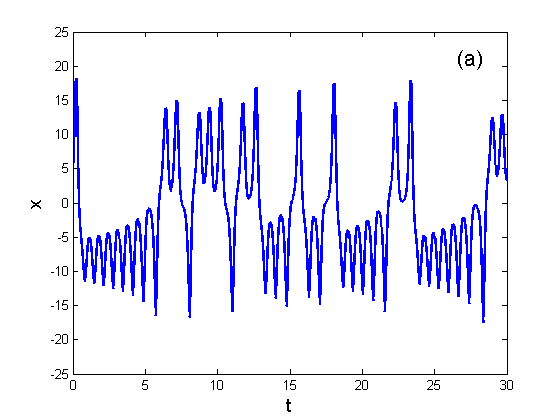
\includegraphics{Figuras/lorenzst.png}} \resizebox{7.2cm}{!}{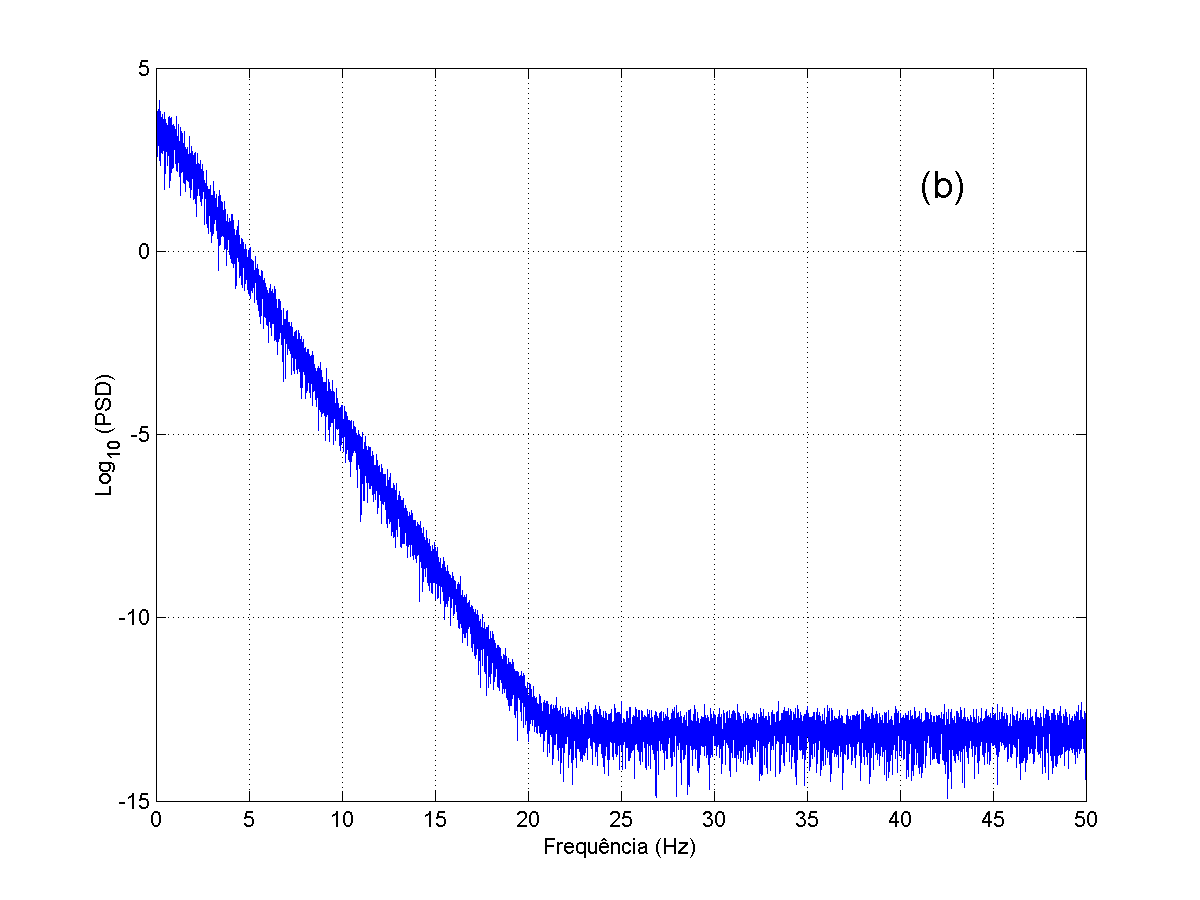
\includegraphics{Figuras/lorenzespectrogrid.png}} \\  \resizebox{7.2cm}{!}{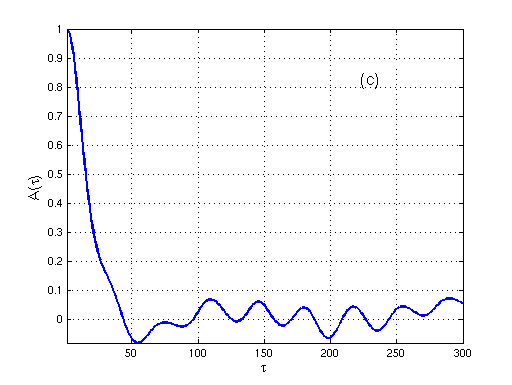
\includegraphics{Figuras/lorenzautocorrgrid.png}} 
\caption{(a) Série temporal caótica da variável $x$ que é parte da solução do sistema~(\ref{eqsistemalorenzpart}). (b) Espectro de potência para a série temporal representada em (a). (c) Função de autocorrelação para a série temporal representada em (a).}
\label{lorenzespec}
\end{figure}

A função de autocorrelação $A(\tau)$ da série temporal~(\ref{eqserietemp}) é definida como

\begin{equation}
A(\tau)=\frac{1}{N-\tau}\sum_{n=1}^{N-\tau}\frac{\left(x_{n}-\overline{x}\right)\left(x_{n+\tau}-\overline{x}\right)}{\sigma^2}
\label{eqautocorr}
\end{equation}
onde $N$ é o número de pontos da série, $\overline{x}$ sua média e $\sigma^2$ sua variância. Essa função representa a média do produto dos valores da série temporal nos instantes $t$ e $t+\tau\Delta t$ e indica por quanto tempo o valor da série temporal no instante $t$ depende de seus valores prévios; em outras palavras $A(\tau)$ mede o grau de semelhança existente no sinal à medida que o tempo passa~\cite{gollub/98}. 

A função de autocorrelação~(\ref{eqautocorr}) pode ser utilizada na análise de uma série temporal irregular. Se a série temporal~(\ref{eqserietemp}) é periódica ou quasiperiódica a função de autocorrelação $A(\tau)$ permanece diferente de zero quando o tempo (ou $\tau$) tende ao infinito. $A(\tau)$ de um sinal periódico é igualmente periódica, pois o sinal periódico volta a se parecer consigo mesmo após um intervalo de tempo correspondente ao período. Já para sistemas caóticos $A(\tau)\rightarrow 0$ quando $\tau\rightarrow \infty$~\cite{argyris/94}; a semelhança de uma série temporal consigo mesma diminui com o tempo e acaba por desaparecer completamente (ver Figura~\ref{lorenzespec}(c)).
A função de autocorrelação de um sinal multi-periódico com muitas freqüências independentes e incomensuráveis também se confunde com aquela de um sinal caótico, e desta forma a caracterização de comportamento, com base na função de autocorrelação, é comprometida.

A Figura~\ref{lorenzespec}(c) apresenta a função de autocorrelação associada à variável $x$, que é parte da solução do Sistema~(\ref{eqsistemalorenzpart}). Pode-se observar que $A(\tau)\rightarrow 0$ quando $\tau\rightarrow \infty$, e desta forma, a semelhança da série temporal consigo mesma diminui com o tempo e acaba por desaparecer completamente. Este comportamento é necessário, mas não suficiente para a caracterização de uma dinâmica caótica na série temporal em estudo.

A análise tradicional de séries temporais baseada na análise do espectro de potências ou da função de autocorrelação não permite, em geral, a distinção entre uma dinâmica caótica determinística e comportamento estocástico. Vários processos têm sido desenvolvidos com essa finalidade, inclusive nos casos em que não se sabe (ou não é possível) modelar ou descrever a dinâmica em termos de equações diferenciais ou mapas. Esse assunto será abordado em detalhes na Seção~\ref{subsecreconst}.

\subsection{A reconstrução do espaço de fase}

\label{subsecreconst}
Métodos para análise dinâmica de séries temporais com comportamento caótico estão ainda em desenvolvimento. Porém, um método comum é um processo dividido em duas partes~\cite{gollub/98}: 
\begin{enumerate}
\item reconstrução do atrator caótico de um sistema dinâmico desconhecido por meio de uma série temporal;

\item determinação de certas quantidades invariantes do sistema por meio do atrator reconstruído. Estes invariantes podem incluir um ou mais expoentes de Lyapunov e a dimensão do atrator. 
\end{enumerate}

Os dois processos acima citados são baseados na reconstrução do espaço de fase, que tem provado ser uma ferramenta poderosa na análise de sistemas físicos não-lineares com comportamento caótico~\cite{argyris/94}. A idéia básica desta reconstrução está calcada no fato de que a história temporal de uma série temporal contém informações sobre variáveis de estado não observáveis que podem ser usadas para determinar um estado presente. As idéias fundamentais sobre esta técnica são creditadas a \citeonline{packard/80} e \citeonline{tak/81} e uma de suas principais características é a preservação dos invariantes do sistema (dimensão do atrator e expoentes de Lyapunov).

A primeira tentativa de reconstruir um atrator caótico por meio da evolução de uma única variável de estado foi realizada por \citeonline{packard/80}. Esses autores analisaram o comportamento do sistema dinâmico de Rössler\footnote{O modelo de Rössler que satisfaz o sistema de EDO's: $dx/dt=-y-z;dy/dt=x+0.2y;dz/dt=0.4+(x-5.7)z$ possui um atrator caótico em seu espaço de fase.} no espaço de fase formado pelos eixos $x,dx/dt$ e $d^{2}x/dt^2$. Eles mostraram que, nesse novo espaço, a figura geométrica que caracteriza o comportamento assintótico do sistema é topologicamente equivalente ao atrator caótico original. Essa figura é chamada \textit{atrator reconstruído}. Assim, o atrator original (no espaço $x,y,z$) e o atrator reconstruído (no espaço $x,dx/dt,d^{2}x/dt^{2}$) são caracterizados pelos mesmos valores de dimensões e expoentes de Lyapunov. Portanto, a partir da evolução temporal de uma única variável de estado, $x(t)$ neste caso, pode-se determinar as características do atrator associado. Segundo os autores, essa idéia pode ser utilizada para qualquer sistema dinâmico que possui um atrator caótico em seu espaço de fase, como por exemplo o sistema de Lorenz (ver Figura~\ref{lorenzdiff}).

\begin{figure}[ht]
\centering 
\resizebox{15cm}{!}{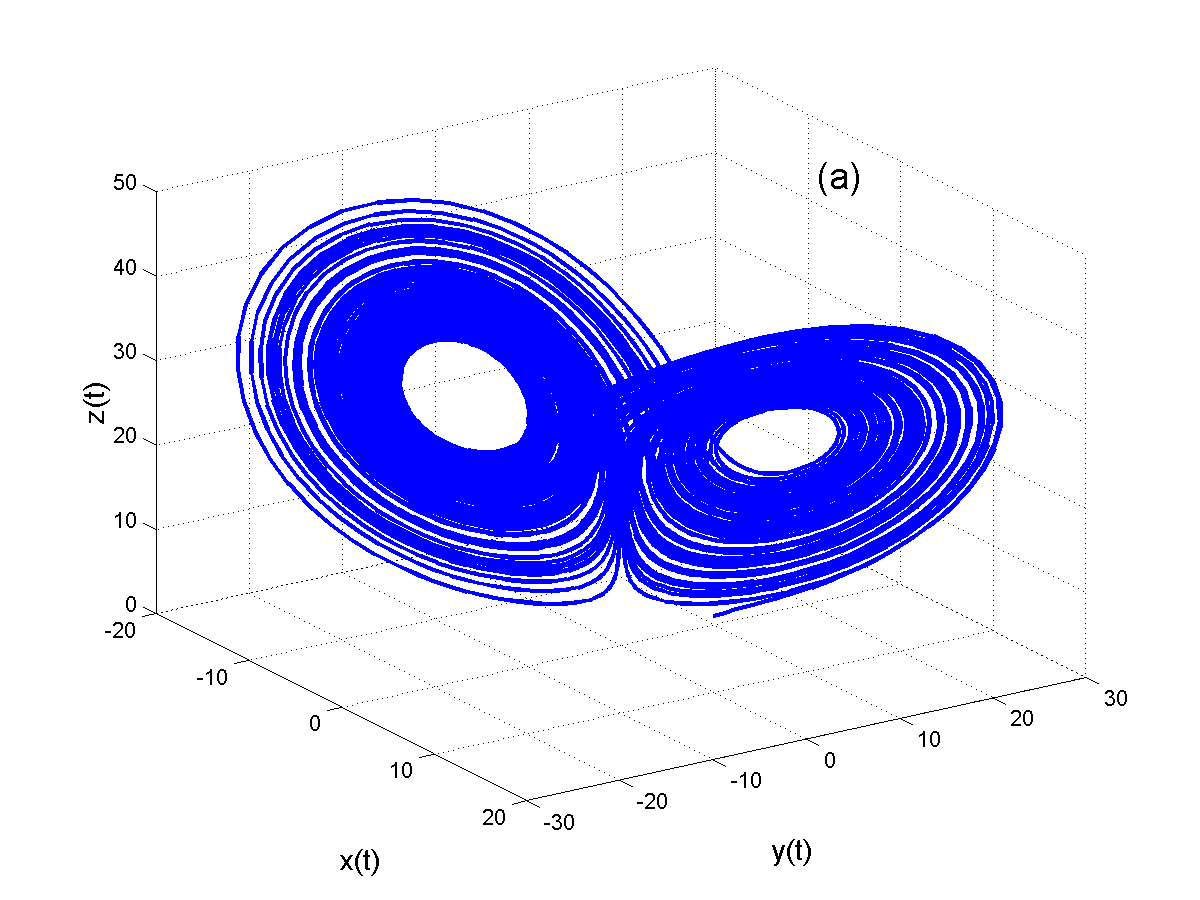
\includegraphics{Figuras/lorenzpack1.png}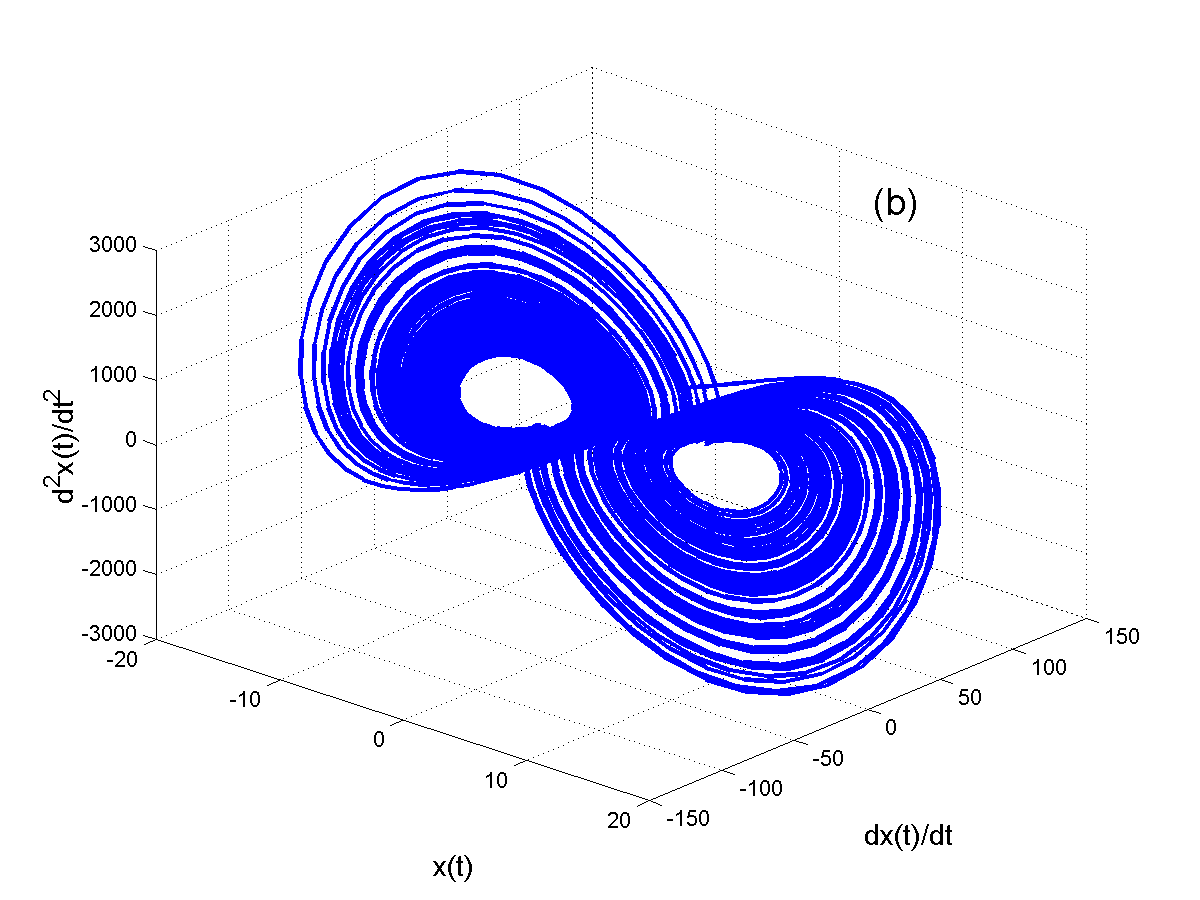
\includegraphics{Figuras/lorenzpack2.png}}
\caption{Atrator de Lorenz para o Sistema~(\ref{eqsistemalorenzpart}). (a) Atrator original. (b) Atrator reconstruído pelo método das derivadas.}
\label{lorenzdiff}
\end{figure}

As derivadas $dx/dt,d^{2}x/dt^{2}$ ou de ordens superiores podem ser aproximadas por equações de diferenças com passo pequeno. Assim:

\begin{equation}
\begin{array}{rcll} \dfrac{dx}{dt} & \simeq & \dfrac{x(t+h)-x(t)}{h} & h\rightarrow 0 \\ 
                     & & &  \\
                    \dfrac{d^{2}x}{dt^{2}} & \simeq & \dfrac{x(t+2h)-2x(t+h)+x(t)}{h^2} & h\rightarrow 0 
\end{array}
\label{eqderivadapack}
\end{equation}

A determinação numérica de derivadas a partir de um conjunto discreto de pontos é bastante sensível ao ruído, o que torna seu cálculo muito impreciso. Além disso, o passo $h$ possui um valor finito, de maneira que a qualidade da aproximação de uma derivada por uma equação de diferença diminui com o aumento da ordem da derivada~\cite{monteiro/02}. Desta forma, tal algoritmo torna-se pouco prático, principalmente se o número de variáveis de estado envolvido for grande.

Os problemas constatados com o método de \citeauthoronline{packard/80} são evitados utilizando-se um procedimento proposto por \citeonline{tak/81}. Takens provou que, no espaço de fase formado pelos eixos $x(t),x(t+\tau),x(t+2\tau),\ldots,x(t+(m-1)\tau)$, o atrator reconstruído é topologicamente equivalente ao atrator ``real'', sobre o qual conhece-se apenas a evolução em tempo discreto da variável de estado $x$. Na sua prova, Takens assumiu que a série é formada por infinitos pontos e que não há ruído. Segundo Takens, se essas condições são satisfeitas, as propriedades topológicas do atrator reconstruído são preservadas, e a reconstrução do mesmo é feita com base na relação:

\begin{equation}
m\geq 2D_{0}+1,
\label{eqconditak}
\end{equation}
onde $D_{0}$ é a dimensão de contagem de caixas do atrator associado.
 
Contudo, sua condição é suficiente mas não necessária, e, desta forma, a dimensão do atrator reconstruído pode obedecer a relação $m\geq D_{0}+1$ \cite{ding/93a}. Chama-se \textit{espaço de imersão} (``embedding space'') o espaço no qual realiza-se a reconstrução. Denomina-se $m$ de \textit{dimensão de imersão} (``embedding dimension'') e $\tau$ o \textit{passo da reconstrução} ou \textit{tempo de atraso} (``time delay''). Note que $\tau$ deve ser um múltiplo do espaçamento (ou tempo de amostragem) $\Delta t$ dos pontos da série temporal.

Pelo \textit{método dos atrasos temporais} de Takens, a cada instante $t_{i}$, assinala-se o ponto de coordenadas $x(t_{i}),x(t_{i}+\tau),\ldots,x(t_{i}+(m-1)\tau)$ no espaço de imersão. Variando-se $i$ de $1$ até $N$, obtém-se a trajetória reconstruída. Supondo que $\vec{\xi}_{\alpha}$ represente a posição do ponto no espaço de imersão no instante $t_{\alpha}$, a trajetória reconstruída é formada pela seqüência:

\begin{equation}
\vec{\xi}_{\alpha}=(x(t_{\alpha}),x(t_{\alpha}+\tau),x(t_{\alpha}+2\tau),...,x(t_{\alpha}+(m-1)\tau))
\label{eqtakensreconst}
\end{equation} 
com $\alpha=1,\ldots,M$. As constantes $m,\tau,N,M$ relacionam-se por $N=M+(m-1)\tau$. Assumindo que a série temporal é o resultado de um processo determinístico, cada $\vec{\xi}_{\alpha+1}$ é o resultado de um mapeamento desconhecido, $\mathcal M(\vec{\xi}_{\alpha})$, ou seja,

\begin{equation}
\vec{\xi}_{\alpha+1}=\mathcal M(\vec{\xi}_{\alpha})
\label{eqtakensreconst2}
\end{equation} 

\subsubsection{A escolha do passo}

\citeonline{tak/81} demonstrou que para um número infinito de pontos e na ausência de ruído a escolha do passo de reconstrução $\tau$ é na grande maioria dos casos arbitrária. Entretanto, as séries temporais experimentais são finitas, usualmente contaminadas com ruído externo e obtidas com o uso de filtros. Nessa situação, a reconstrução depende da escolha correta do passo. Se o passo $\tau$ for muito pequeno $x(t),x(t+\tau)$ e $x(t+2\tau)$, por exemplo, terão praticamente o mesmo valor\footnote{Admite-se que a freqüência de amostragem, relacionada com o intervalo de tempo $\Delta t$ entre duas medidas consecutivas, é suficientemente elevada para capturar toda a estrutura fina do sinal, ou seja, que ela seja adequada para se monitorar com detalhe a evolução temporal do sistema.}. Como conseqüência, o atrator reconstruído fica comprimido em torno da diagonal $z=y=x$, já que $\vec{\xi}_1\simeq\vec{\xi}_2\simeq\vec{\xi}_3$, ou seja, esse atrator apresentará uma dependência linear entre $\vec{\xi}_1,\vec{\xi}_2$ e $\vec{\xi}_3$, que não ocorre nas componentes reais $x,y$ e $z$ (conforme Figura~\ref{figlorenzpasso}(a)). Por outro lado, como a trajetória real está restrita a um volume finito do espaço de fase, o passo $\tau$ não pode ser muito grande, sob pena dos vetores reconstruídos $\vec{\xi}_i$ serem completamente não-correlacionados, cobrindo todo o espaço de fase (conforme Figura~\ref{figlorenzpasso}(c)).

\begin{figure}[ht]
\centering 
\resizebox{7.2cm}{!}{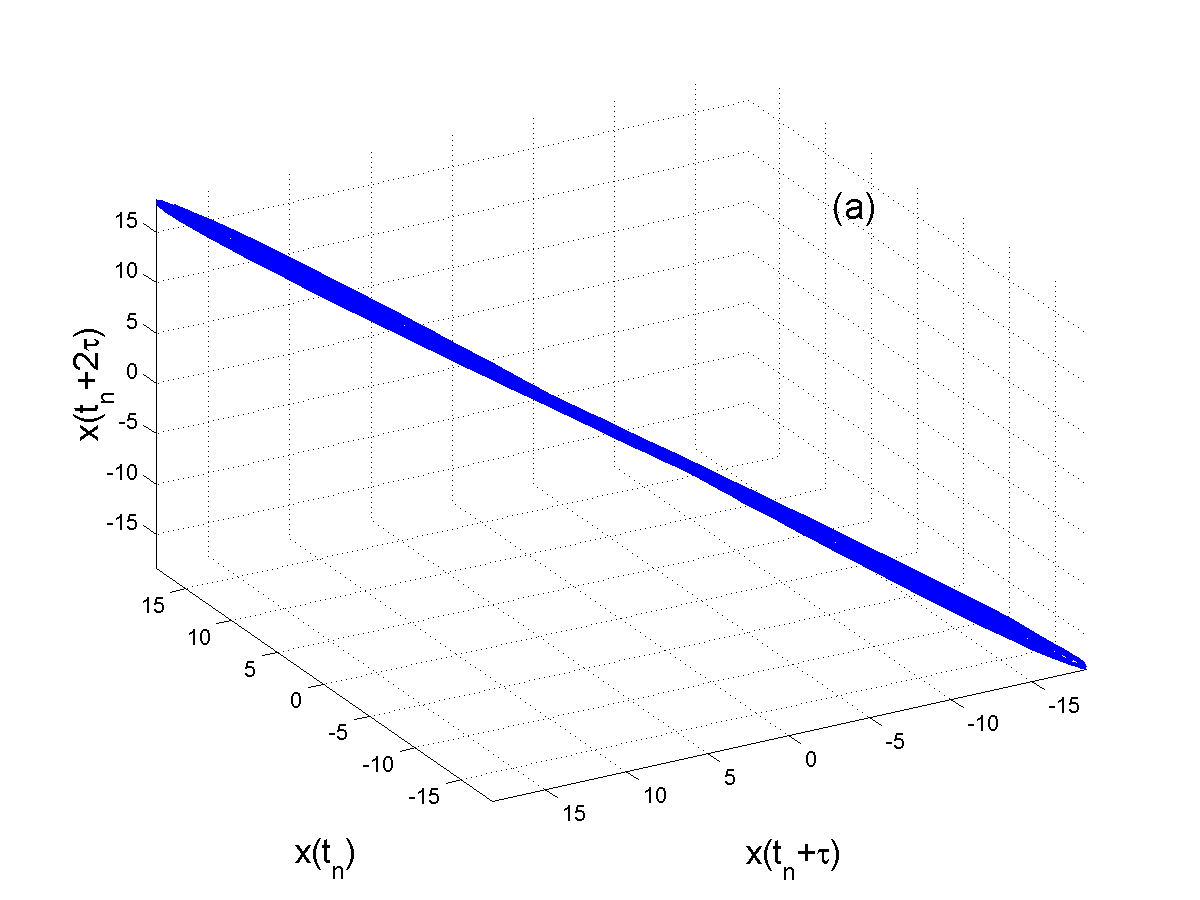
\includegraphics{Figuras/lorenzatraso1.png}} \resizebox{7.2cm}{!}{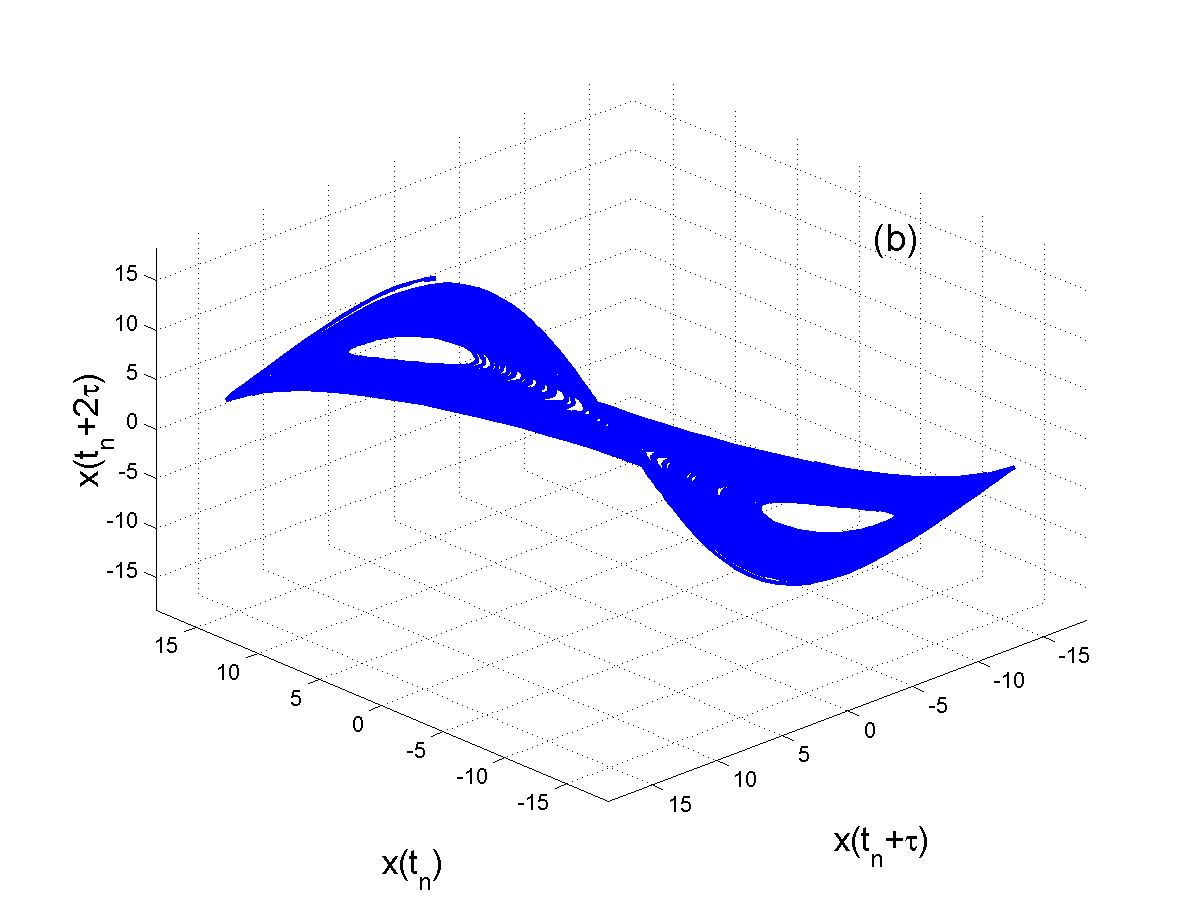
\includegraphics{Figuras/lorenzatraso2.png}} \\  \resizebox{7.2cm}{!}{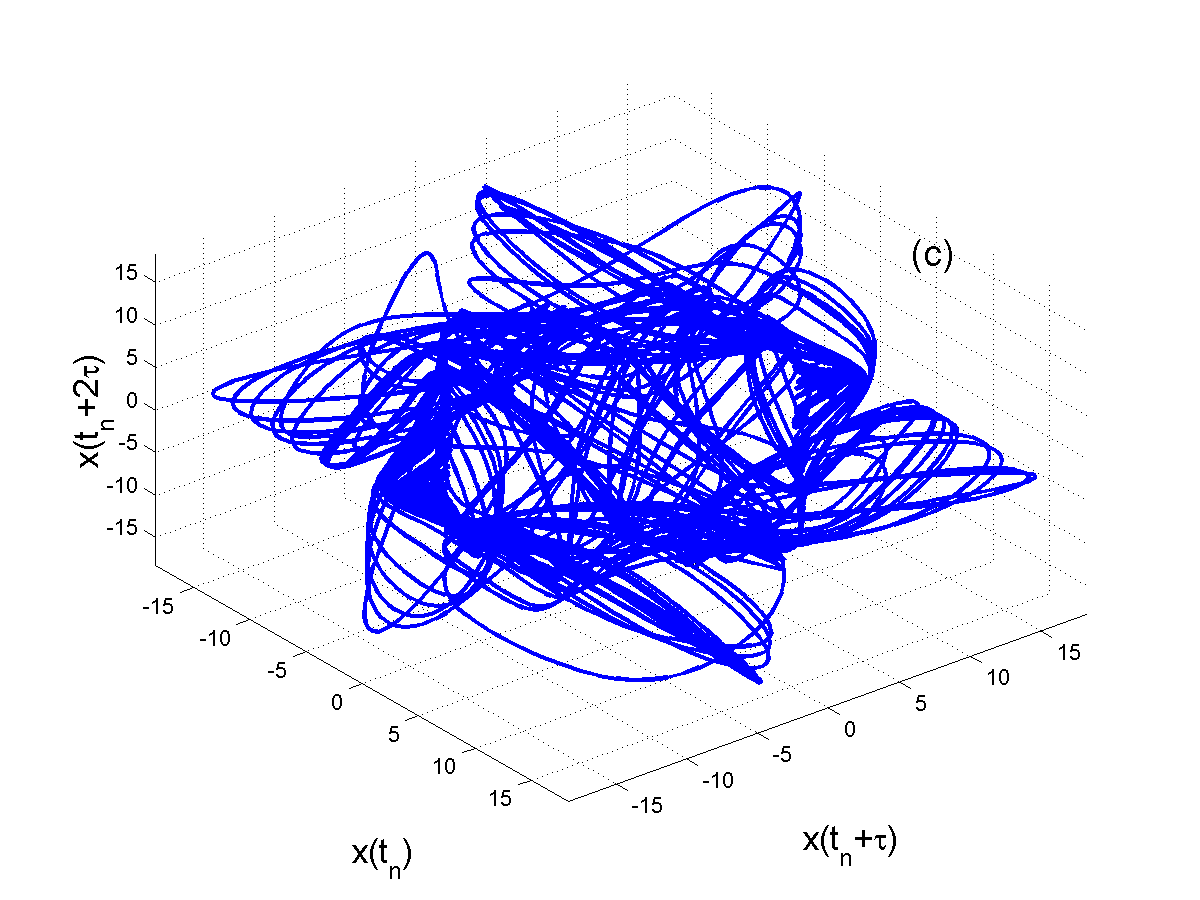
\includegraphics{Figuras/lorenzatraso3.png}} 
\caption{Exemplo da influência do passo na reconstrução do atrator de Lorenz associado ao Sistema~(\ref{eqsistemalorenzpart}). (a) passo muito pequeno ($\tau=1$). (b) passo adequado ($\tau=12$). (c) passo muito grande ($\tau=50$).}
\label{figlorenzpasso}
\end{figure}

Diversos trabalhos têm proposto critérios para orientar a escolha do passo correto~\cite{fraswi/86}. O critério mais difundido, e também utilizado nesta dissertação, consiste em examinar a correlação entre os pares de pontos em função de seu tempo de separação, ou seja, através da função de autocorrelação (já definida na Seção~\ref{secanalisetrad}). Após determinar o tempo do primeiro ``zero'' desta função, uma modesta fração deste valor é uma escolha razoável para o atraso $\tau$ \cite{gollub/98}.

A sensibilidade do processo de reconstrução relativamente ao passo pode ser estimada através de um método bastante prático e rápido: o chamado \textit{gráfico de primeiro retorno}, que consiste em graficar-se $x(t_{i})\times x(t_{i}+\tau)$, reconstruindo-se para tanto vetores bidimensionais com passo $\tau$ (conforme Figura~\ref{figlorenzprimeiroret}). Uma simples inspeção visual desse gráfico fornece informações sobre os valores de $\tau$ para os quais $x(t_{i})$ e $x(t_{i}+\tau)$ está ainda fortemente correlacionados, situação em que o atrator reconstruído fica comprimido próximo à diagonal e, desta forma, indica quão sensível é a reconstrução do atrator relativamente à escolha do passo, quão homogêneo é o atrator e qual o número típico de vetores reconstruídos necessário para caracterizá-lo completamente~\cite{monteiro/02}. 

\begin{figure}[ht]
\centering 
\resizebox{7.2cm}{!}{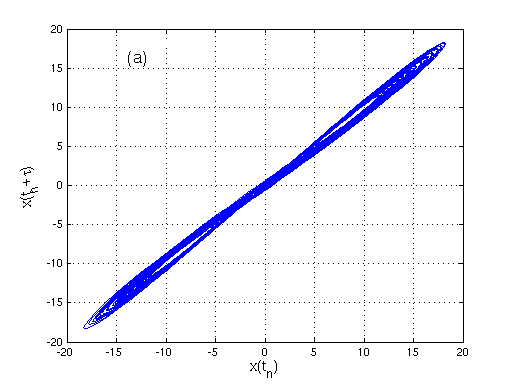
\includegraphics{Figuras/lorenzreconstbi1.png}} \resizebox{7.2cm}{!}{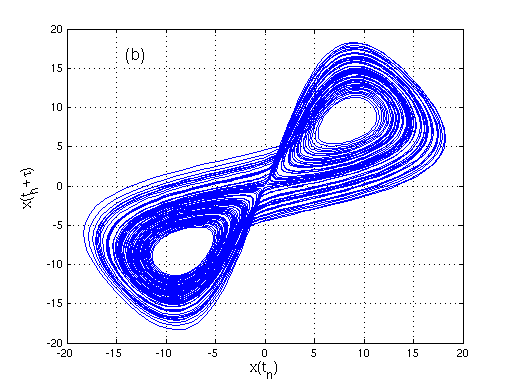
\includegraphics{Figuras/lorenzreconstbi12.png}} \\  \resizebox{7.2cm}{!}{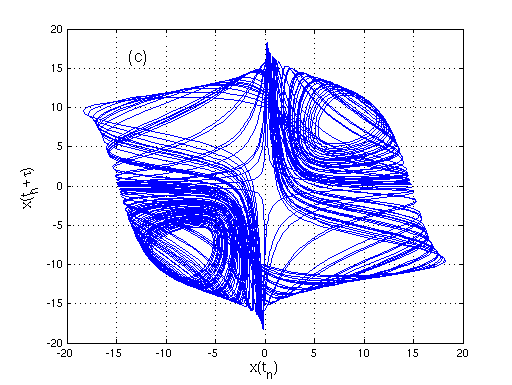
\includegraphics{Figuras/lorenzreconstbi50.png}} 
\caption{Gráfico de primeiro retorno a partir da variável $x$ que é parte da solução do Sistema~(\ref{eqsistemalorenzpart}). (a) $\tau=1$. (b) $\tau=12$. (c) $\tau=50$.}
\label{figlorenzprimeiroret}
\end{figure}

\subsubsection{A escolha da dimensão de imersão}
\label{secdimimers}

\paragraph*{Dimensões generalizadas}
Atratores caóticos apresentam um comportamento irregular e os mesmos não preenchem completamente o espaço de fase devido à contração do elemento de volume~\cite{argyris/94}. Um atrator caótico imerso em um espaço de fase tridimensional é uma forma ``híbrida'' entre uma superfície e um objeto espacial e assim sua dimensão está entre $2$ e $3$, ou seja, é um fractal. Desta forma, a caracterização desse atrator é realizada com base no conceito generalizado de dimensão que no caso de atratores regulares como pontos fixos, ciclos limites e toros, coincidem com a dimensão convencional em geometria euclidiana, ou seja, $0$, $1$ ou $2$.

Existe um conjunto infinito de dimensões, $D_{q}$, conhecidas como dimensões generalizadas, que definem propriedades métricas ou probabilísticas de um atrator~\cite{hentschel/83}. Deixe um atrator caótico ser coberto por $m(\varepsilon)$ quadrados de lado $\varepsilon$, e seja $M$ o número total de pontos observados no atrator. Então, a probabilidade de que um ponto se encontre no $i$-ésimo quadrado é obtido pela razão $p_{i}=M_{i}/M$, onde $M_{i}$ é o número de pontos do atrator que se encontra no $i$-ésimo quadrado. O conjunto infinito de dimensões generalizadas é dado por

\begin{equation}
D_{q}=\dfrac{1}{q-1}\lim_{\varepsilon\rightarrow\infty}\dfrac{\ln \sum_{i=1}^{m(\varepsilon)}p_{i}^q}{\ln \varepsilon}
\label{eqdimgeneral}
\end{equation}

onde $q$ está relacionado às possíveis definições da dimensão. Quando $q=0$, a relação~(\ref{eqdimgeneral}) produz simplesmente a dimensão de contagem de caixas $D_{0}$ sobre o atrator. A dimensão de informação $D_{1}$ e a dimensão de correlação $D_{2}$ são obtidas no limite da Equação~(\ref{eqdimgeneral}) quando $q$ tende para $1$ e $2$, respectivamente. $D_{1}$ pode ser expresso como~\cite{farmer/83}

\begin{equation}
D_{1}=\lim_{\varepsilon\rightarrow 0}\dfrac{\ln \sum_{i=1}^{m(\varepsilon)}p_{i} \ln p_{i}}{\ln \varepsilon}
\label{eqdiminfor}
\end{equation}

que é conhecida como dimensão de informação ou dimensão entrópica.

A dimensão de correlação, proposta por \citeonline{grassproca/83} como uma forma de caracterizar atratores caóticos, é dada pela relação

\begin{equation}
D_{2}=\lim_{r\rightarrow\ 0}\frac{\log C(r)}{\log r}
\label{eqcorr2}
\end{equation}
onde $C(r)$ é a função de correlação integral definida como

\begin{equation}
C(r)=\frac{1}{M^2}\sum_{i,j=1 \\, i\neq j}^{M} \Theta\left(r-\left \|\vec{\xi}_{i}-\vec{\xi}_{j}\right \|\right),
\label{eqcorr1}
\end{equation}
onde $M$ é o número de pontos no atrator, $\|\|$ denota a norma euclidiana que quantifica a distância entre os pares de vetores em espaços de imersão arbitrários e $\Theta(x)$ é uma função degrau de Heavyside, definida por
\begin{equation}
\Theta(x)=\
\left\{ \begin{array}{ccl}
 1,  &  \mathrm{se} & x\geq 0   \\
 0,  &  \mathrm{se} & x< 0
\end{array}
\right.  
\label{eqheavyside}
\end{equation}

A correlação integral (\ref{eqcorr1}) conta a freqüência relativa de pares cuja separação é menor que a escala $r$. Note que a Equação~(\ref{eqcorr2}) implica que para pequenos valores de $r$, a correlação integral $C(r)$ comporta-se como uma lei de potência $C(r)\approx r^{D_{2}}$. Conseqüentemente, o cálculo do expoente pode ser obtido a partir de um gráfico de $C(r)$ versus $r$ em escala $\log$-$\log$.

Para valores de $q\geq3$, \citeonline{hentschel/83} fornecem aproximações para as dimensões generalizadas $D_{3},D_{4},\ldots$ associando funções de correlação integral entre triplas, quádruplas, etc. de vetores. É possível mostrar que estas dimensões estão ordenadas da seguinte maneira: $D_{0}\geq D_{1}\ldots\geq D_{n}$, sendo que a igualdade é válida sob a hipótese de que os pontos do atrator sejam uniformemente distribuídos.

Em geral, o expoente $D_{2}$ é mais fácil de ser estimado que o expoente $D_{0}$ devido ao grande esforço computacional empregado na procura da dimensão de contagem de caixas~\cite{greenside/82}. Em diversos sistemas, a dimensão de contagem de caixas $D_{0}$ e a dimensão de correlação $D_{2}$ são muito próximas uma da outra e, desta maneira, o valor de $D_{2}$ fornece uma boa estimativa do número mínimo de equações diferenciais não-lineares necessárias para descrever o atrator~\cite{moon/97}.

% Na prática, para um conjunto finito de dados com resolução temporal discreta e finita exatidão, o limite em (\ref{eqcorr2}) pode não ser rigorosamente alcançado. Porém, em um gráfico de $\log C(r,M)$ versus $\log r$, uma parte linear aparece para valores intermediários de $r$. Sua inclinação fornece uma estimativa da dimensão de correlação \cite{rudolf/95}.

% Conforme a Figura~\ref{lorenzdiff}(a) o atrator de Lorenz cuja dimensão fractal é de aproximadamente $d=2.16$, pode ser bem representado em um espaço de imersão $m=3$. Contudo, em uma série temporal arbitrária a dimensão $d$ do atrator é desconhecida e, desta forma, o valor $m$ também o é. 

A implementação do algoritmo de Grassberger-Procaccia é relativamente simples. Entretanto, esse algoritmo  exige o cálculo e a classificação de aproximadamente $n(n-1)$ distâncias, onde $n$ é o número de vetores reconstruídos pela relação~(\ref{eqtakensreconst}). Este procedimento consome um tempo de processamento  excessivamente longo se o algoritmo não é construído  de forma otimizada, sobretudo se a série temporal for muito longa. Diversas sugestões, simplificações e modificações têm sido propostas~\cite{theiler/87,parker/89,malraison/83}. O procedimento adotado nesta dissertação reduz o cálculo de distâncias por considerar apenas um subconjunto de vetores reconstruídos, escolhidos de forma aleatória~\cite{malraison/83}. Como a escolha é aleatória, espera-se que o subconjunto de distâncias calculadas reproduza a estatística do conjunto de todas as distâncias, mantendo inalterado o valor de $C(r)$.

Na medida em que há limitações experimentais fortes para a obtenção de séries de dados longas, esse fato, aliado ao excessivo tempo de processamento, restringe a utilização do algoritmo de Grassberger-Procaccia para o caso de atratores de alta dimensão. Na grande maioria das aplicações a sinais experimentais, o algoritmo de Grassberger-Procaccia não permite estimar com segurança dimensões de correlações $D_{2}$ maiores de $4$ e $5$, as quais correspondem a dimensões de imersão da ordem de $9$ e $11$, respectivamente. 

A dimensão de correlação $D_{2}$ é uma das principais ferramentas usadas para identificar a existência de dinâmica caótica. Caos determinístico, em geral, é identificado se a inclinação de $C(r)$ versus $r$ converge para um valor de saturação, para valores cada vez mais altos da dimensão de imersão $m$ \cite{grassproca/83}. Em sinais determinísticos com comportamento caótico, o valor $D_{2}$ alcança um valor máximo devido a natureza de baixa dimensão do sistema. Desta forma, a dimensão de saturação obtida é uma aproximação para a dimensão fractal do atrator. A partir da relação~(\ref{eqconditak}), o valor da dimensão de imersão $m$ pode ser estimado. O valor desta dimensão permite ``desdobrar'' o atrator adequadamente, de modo que suas trajetórias não se cruzem no espaço de imersão. 

A Figura~\ref{figatratorhipot} ilustra o atrator de Lorenz imerso em espaços de fase de dimensões $2$ e $3$, respectivamente. A imersão no espaço de fase de duas dimensões dá origem a falsos cruzamentos das trajetórias (conforme Figura~\ref{figatratorhipot} (a)). Esses falsos cruzamentos podem estar ligados a falsos vizinhos próximos - um efeito que produz erros no cálculo do expoente de Lyapunov. Somente o espaço de fase tridimensional esboça este atrator completamente (conforme Figura~\ref{figatratorhipot} (b)). Este fato mostra a importância da imersão do atrator reconstruído em um espaço de fase adequado.

\begin{figure}[ht]
\centering 
\resizebox{15cm}{!}{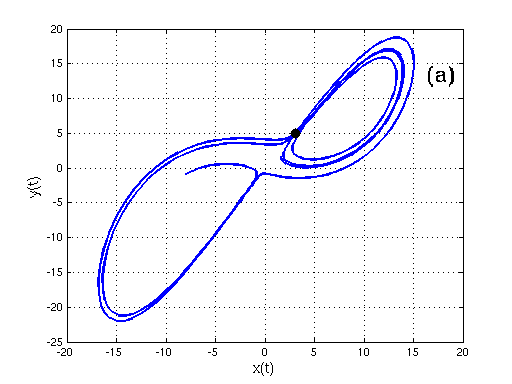
\includegraphics{Figuras/lorenzproj1.png}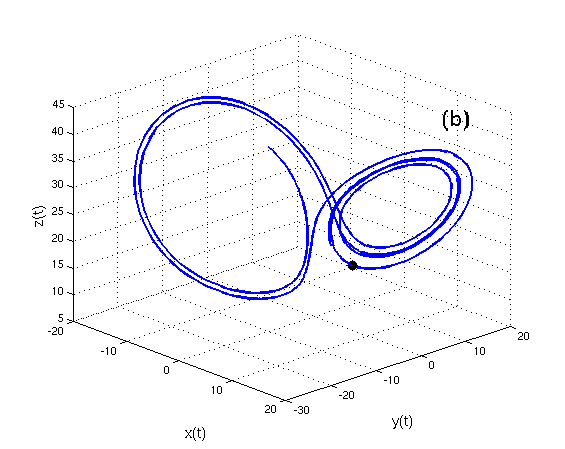
\includegraphics{Figuras/lorenzproj2.png}}
\caption{Efeito da imersão do atrator de Lorenz em espaços de diferentes dimensionalidades. (a) A imersão no espaço de fase bidimensional ocorre um falso cruzamento (marcado com um ponto em preto). (b) O atrator é completamente representado no espaço tridimensional.} 
\label{figatratorhipot}
\end{figure}

A Figura~\ref{figlorenzdimensoes}(b) mostra a correlação integral da série temporal em $x$ de Lorenz (Figura~\ref{figlorenzdimensoes}(a)) versus a escala $r$ em diferentes dimensões de imersão. Pode-se observar que cada uma destas curvas possui seções lineares, cujos valores das inclinações, calculados via regressão linear, saturam quando as dimensões de imersão são incrementadas. Estes valores de inclinações em função das dimensões de imersão que variam de $1$ a $10$ podem ser vistos através da Figura~\ref{figlorenzdimensoes}(c). Foram feitas $5$ realizações análogas à descrita acima, e a dimensão de correlação média obtida foi de $\langle D_{2}\rangle=2.105$ com desvio padrão de $\sigma_{D_{2}}=0.01$. Ainda, na Figura~\ref{figlorenzdimensoes}(c) pode ser observada a dimensão de correlação obtida a partir de uma série temporal aleatória (ruído branco). Para este caso, o valor de $D_{2}$ não satura quando as dimensões de imersão são incrementadas. Este comportamento já era esperado, pois um ruído branco está associado a um processo estocástico e não a uma dinâmica caótica.

\begin{figure}[ht]
\centering 
\resizebox{7.2cm}{!}{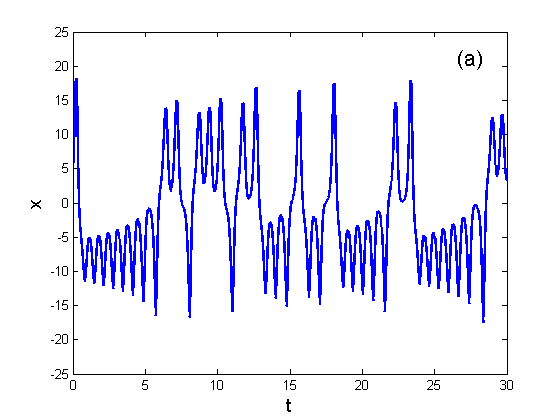
\includegraphics{Figuras/lorenzst.png}} \resizebox{7.2cm}{!}{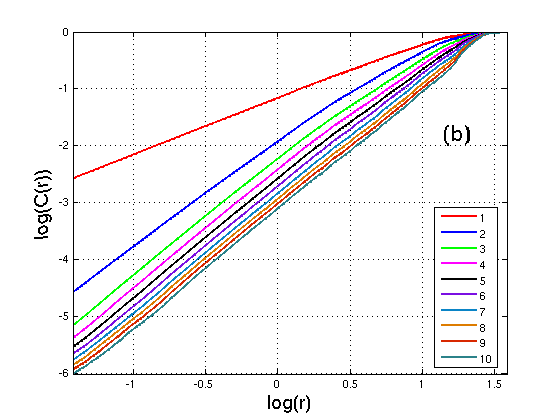
\includegraphics{Figuras/lorenzcorrelint2.png}} \\  \resizebox{7.2cm}{!}{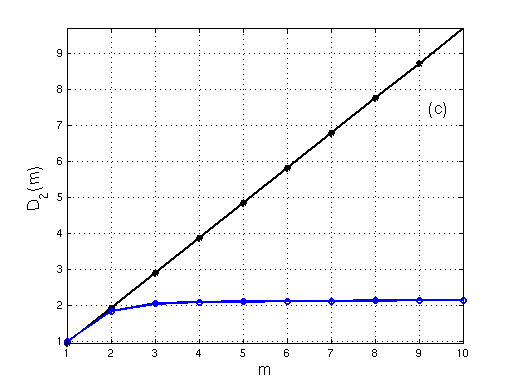
\includegraphics{Figuras/lorenzdimcorrel2.png}} 
\caption{(a) Série temporal obtida a partir da integração do Sistema~(\ref{eqsistemalorenzpart}). (b) Correlação integral da série em (a) com $m=1$ a $10$. (c) Dimensão de correlação de $D_{2}\langle2.105\rangle$ para a série de Lorenz (curva -o- em azul) e dimensão de correlação infinita para uma série aleatória (curva -*- em preto)}
\label{figlorenzdimensoes}
\end{figure}

\paragraph*{Distinção entre dinâmica de baixa dimensão e aleatoridade}

\citeonline{osboproven/89} oferecem um contra-exemplo da visão tradicional de que a inclinação de $C(r)$ versus $r$ aumenta continuamente para processos estocásticos, quando a dimensão de imersão $m$ é incrementada~\cite{grassproca/83}. Especificamente, tais autores mostraram que uma classe simples de ruído ``colorido'', caracterizado por uma lei de potência no espectro da forma $S(w)\approx w^{-\alpha}$ conduz à saturação em $D_{2}$ conforme a relação $D_{2}=2/(\alpha-1)$~\cite{osboproven/89,theilerj/91}. Este resultado tem sérias implicações sobre o estudo experimental de comportamento caótico determinístico, já que a observação de um valor finito de $D_{2}$ pode não ser suficiente para afirmar a presença de atratores caóticos em um sistema dinâmico. 

Em contrapartida, \citeonline{provenzalesmith/92} apresentam alguns testes que podem ser usados na distinção entre dinâmica de baixa dimensão e aleatoriedade em séries temporais. Esses testes são baseados na idéia de se modificar algumas propriedades de uma série temporal, com o intuito de verificar se a convergência de $D_{2}$ depende ou não dessas propriedades modificadas. 

O primeiro de tais testes é denominado ``teste surrogate'' e consiste em considerar a distribuição das fases de Fourier de uma série temporal. Desta forma, é aplicada a transformada de Fourier (conforme a Equação~(\ref{eqfourierdis})) na série em estudo. Em seguida, suas fases são embaralhadas uniformemente e é aplicada a transformada de Fourier inversa. A série temporal obtida com este processo é aleatória, já que o surrogate destrói as correlações existentes na série temporal que lhe deu origem, porém seu espectro de potência é similar ao da série original. Se a convergência de $D_{2}$ é determinada apenas pela forma do espectro (ou equivalentemente pela função de autocorrelação), então os resultados não são afetados pelo embaralhamento das fases. A invariância do valor de $D_{2}$ sobre as fases embaralhadas sugere fortemente que tais estimativas não indicam uma dinâmica caótica~\cite{provenzalesmith/92}. 

A Figura~\ref{figlorenzsurrogate}(a) mostra a série temporal obtida a partir do surrogate da série temporal em $x$ de Lorenz, a Figura~\ref{figlorenzsurrogate}(b) mostra a correlação integral obtida para dimensões de imersão que variam de $1$ a $10$ e finalmente a Figura~\ref{figlorenzsurrogate}(c) apresenta a dimensão de correlação, $D_{2}$, associada. A aparência da série temporal com surrogate é completamente diferente da apresentada na Figura~\ref{figlorenzdimensoes}(a) e os respectivos valores de $D_{2}$ são também bastante distintos (ver Figuras~\ref{figlorenzsurrogate}(c) e \ref{figlorenzdimensoes}(c)). Foram feitas $5$ realizações análogas à descrita acima, e pode-se observar que a dimensão de correlação $D_{2}$ em todos os casos não satura. Esse comportamento sugere fortemente a existência de uma dinâmica de baixa dimensão na série temporal de Lorenz. %Desta forma, em uma série temporal arbitrária, a constatação de um comportamento similar ao encontrado acima \textit{sugere} fortemente a existência de um atrator caótico associado~\cite{provenzalesmith/92}. 

\begin{figure}[ht]
\centering 
\resizebox{7.2cm}{!}{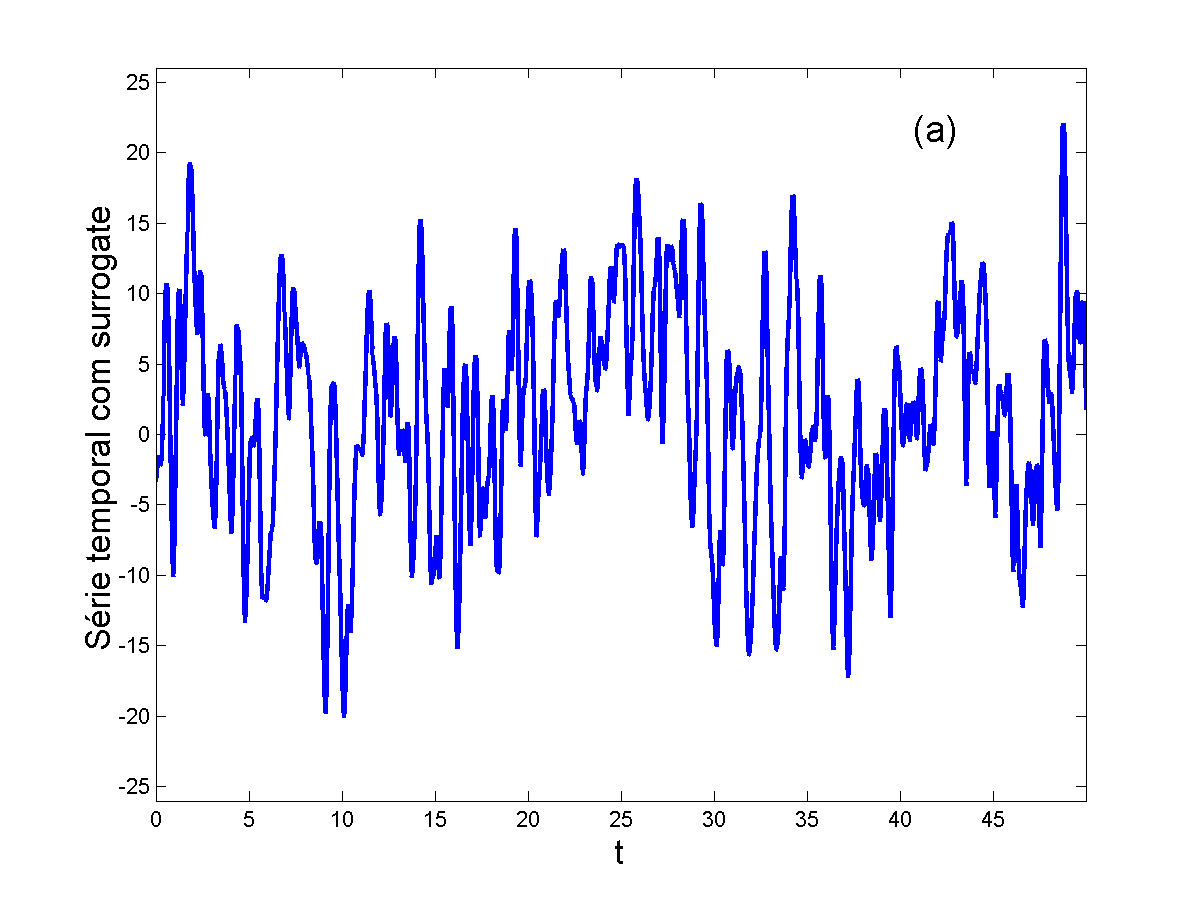
\includegraphics{Figuras/lorenzxsurr.png}} \resizebox{7.2cm}{!}{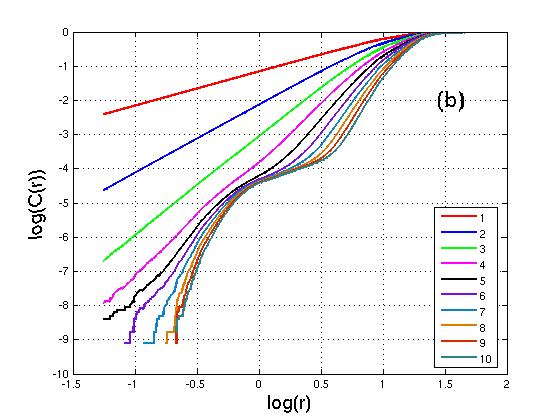
\includegraphics{Figuras/lorenzcorrelint2surr.png}} \\  \resizebox{7.2cm}{!}{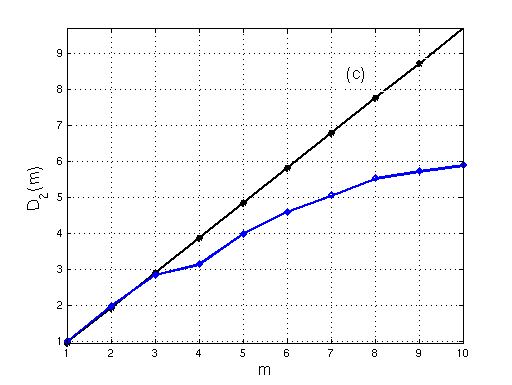
\includegraphics{Figuras/lorenzdimcorrelsurr2.png}} 
\caption{(a) Série temporal de Lorenz em $x$ com fase embaralhada. (b) Correlação integral da série em (a) com $m=1$ a $10$. (c) Dimensão de correlação da série em (a) e dimensão de correlação infinita para uma série aleatória}
\label{figlorenzsurrogate}
\end{figure}

Outro teste consiste em considerar a análise da correlação integral~(\ref{eqcorr1}) da primeira derivada numérica (ou primeira diferença) de uma série temporal. Para um sistema governado por um atrator caótico de baixa dimensão, o valor de $D_{2}$ é o mesmo tanto para a série temporal original quanto para série temporal modificada. Isto porque a primeira derivada numérica (ou primeira diferença) mantem as correlações existentes na série original. 

A Figura~\ref{figlorenzdiff}(a) apresenta a primeira diferença $\Delta x(t)=x(t+\Delta t)-x(t)$ da componente $x$ do atrator de Lorenz, a Figura~\ref{figlorenzdiff}(b) apresenta a correlação integral para $\Delta x$ e a Figura~\ref{figlorenzdiff}(c) apresenta os valores de $D_{2}$ associados. Foram feitas $5$ realizações análogas à descrita acima, e a dimensão de correlação média obtida foi de $D_{2}=\langle2.09\rangle$ com desvio padrão de $\sigma_{D_{2}}=0.03$. Pode-se observar, neste caso, que a dimensão de correlação $D_{2}$ satura em um valor bastante próximo daquela obtido com base na série original. Este comportamento sugere mais uma vez a existência de uma dinâmica de baixa dimensão na série temporal de Lorenz. Ainda, como $D_{2}\thickapprox 2.09$, pela relação de Takens dada por~(\ref{eqconditak}), o atrator de Lorenz pode ser bem representado em um espaço de imersão de $m=6$.

\begin{figure}[ht]
\centering 
\resizebox{7.2cm}{!}{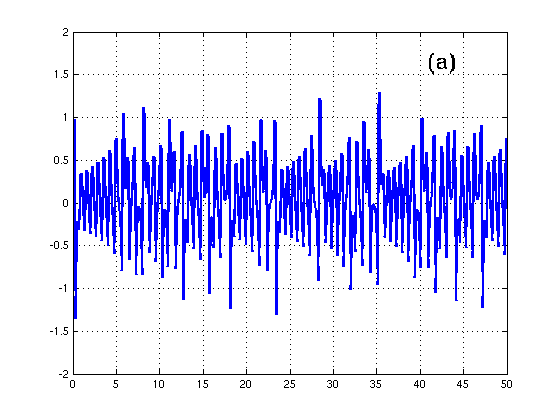
\includegraphics{Figuras/lorenzdiff2.png}} \resizebox{7.2cm}{!}{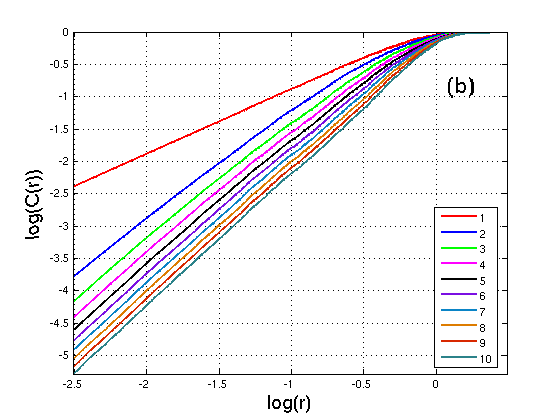
\includegraphics{Figuras/lorenzcorrelintdiff2.png}} \\  \resizebox{7.2cm}{!}{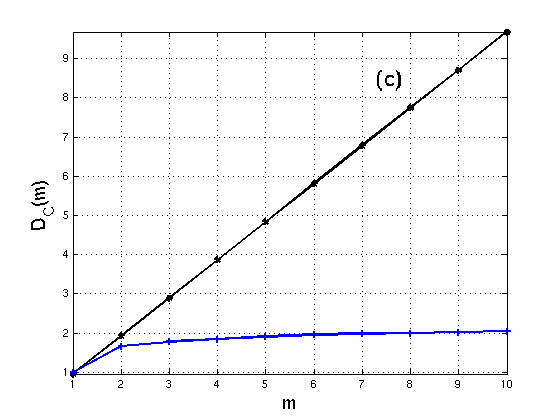
\includegraphics{Figuras/lorenzdimcorreldiff2.png}} 
\caption{(a) Série temporal gerada a partir da primeira diferença da série temporal $x$ de Lorenz. (b) Correlação integral da série em (a) com $m=1$ a $10$. (c) Dimensão de correlação da série em (a) e dimensão de correlação infinita para uma série aleatória.}
\label{figlorenzdiff}
\end{figure}

A técnica de reconstrução do espaço de fase (\ref{eqtakensreconst}) como também o cálculo da dimensão de correlação (\ref{eqcorr2}) devem ser usados após uma avaliação cuidadosa das condições de sua aplicabilidade, seguida de uma avaliação da consistência dos resultados obtidos. Uma aplicação ingênua de tais métodos pode levar a conclusões errôneas~\cite{osboproven/89}. \citeonline{eckruelllyap/92} fornecem evidências segundo as quais o valor de $D_{2}$, estimado a partir do algoritmo de Grassberger-Procaccia, não fornece dimensões confiáveis maiores que:

\begin{equation}
D_{2_{\textrm{max}}}=2\log_{10}N
\label{eqlimitemax}
\end{equation}
onde $N$ é o número de pontos da série temporal. Desta forma, quando o valor da dimensão de correlação satura em um valor superior ao estabelecido pela Equação~(\ref{eqlimitemax}) pode não ser correto afirmar a série temporal possui uma dinâmica de baixa dimensão. Sob essa perspectiva, a dimensão de correlação obtida a partir de $10.000$ pontos da série em $x$ de Lorenz é confiável já que seu valor, a saber $D_{2}\thickapprox 2.1$, satisfaz a relação $D_{2_{\textrm{max}}}\leq 8$.

\subsubsection{Estacionaridade}
\label{subsecestacio}

O estudo das propriedades de um atrator associado a um sistema dinâmico 
admite que o mesmo se encontre em um \textit{estado estacionário}\footnote{Sob o ponto de vista estatístico, uma série temporal é estacionária se a função de densidade de probabilidade associada não se altera ao longo do tempo (estacionaridade plena), ou particularmente se os primeiros momentos associados a uma série temporal, como média e variância não se alteram ao longo do tempo (estacionaridade estrita).}, ou para o caso de um experimento real, muito próximo desse estado - situação em que os pontos representativos da evolução temporal do sistema estão bastante próximos do atrator associado à dinâmica. Desta forma, é importante verificar se a série temporal em estudo corresponde, de fato, a um estado estacionário do sistema físico real~\cite{aguirre/00}.

O critério de estacionaridade utilizada nesta dissertação emprega janelas de dados deslizantes ao longo de uma série. Ou seja, dada uma série temporal~(\ref{eqserietemp}), pode-se definir como janelas de dados deslizantes todos os subconjuntos de amostras subseqüentes possíveis, de comprimento $L$ (conforme Figura~\ref{figestaciogeral}). Testes que envolvem tais janelas procuram analisar e quantificar as propriedades que se alteram ao longo da série temporal, como a média e a variância, com base em um determinado intervalo de confiança~\cite{alvaro/01}.

% \begin{figure}[ht]
% \centering \resizebox{15cm}{!}{\includegraphics{Figuras/figestacionaria.png}}
% \caption{Janelas de dados deslizantes} 
% \FONTE{\cite{alvaro/01}}
% \label{figestaciogeral}
% \end{figure}

\begin{figure}[!ht]
\begin{center}
\resizebox{12cm}{!}{\input{Figuras/estacionariaxfig2.pdftex_t}}
\caption{Janelas de dados deslizantes} 
\end{center}
\label{figestaciogeral}
\end{figure}
 
Desta forma, médias parciais ($\mu_{\textrm{parcial}}$) e variâncias parciais ($\sigma_{\textrm{parcial}}$) devem satisfazer as relações:
\begin{equation}
\begin{array}{rcccl}
\mu_{\textrm{total}}-\sigma_{\textrm{total}} & \leq  &  \mu_{\textrm{parcial}} & \leq  & \mu_{\textrm{total}}+\sigma_{\textrm{total}}\\
&   &   &   &\\
\sigma_{\textrm{total}}^2-\sigma_{\textrm{total}} & \leq  &  \sigma_{\textrm{parcial}}^2 & \leq  & \sigma_{\textrm{total}}^2+\sigma_{\textrm{total}}
\end{array}
\label{eqestacionaria}
\end{equation} 
onde $\mu_{\textrm{total}}$, $\sigma_{\textrm{total}}$ e $\sigma_{\textrm{total}}^2$ são a média, desvio padrão e variância da série temporal, respectivamente.

O teste de estacionaridade descrito acima foi aplicado à série $x$ de Lorenz com janelas deslizantes de comprimento $L=100$. Como todos os valores parciais de $\mu$ e $\sigma$ satisfazem a relação~(\ref{eqestacionaria}) pode-se dizer que tal série é estacionária.


\subsubsection{Os expoentes de Lyapunov}

Em séries temporais experimentais, o ponto de partida para o cálculo dos expoentes de Lyapunov é o atrator reconstruído em uma dimensão de imersão $m$ adequada. Uma vez reconstruído o atrator, define-se uma trajetória de referência (ou trajetória fiducial) a partir da seqüência de vetores reconstruídos. Em seguida, deve-se analisar o que ocorre com pontos vizinhos desta trajetória. Com as informações sobre as taxas de divergência destes pontos, pode-se obter, então, os expoentes de Lyapunov. 

Diversos métodos têm sido propostos para estimar esses expoentes em séries temporais experimentais~\cite{wolf/85,eckrue/86,sanosawada/85}. O método proposto por \citeonline{wolf/85} permite calcular com expressiva precisão o maior expoente de Lyapunov (positivo). Considere uma trajetória descrita pela seqüência de pontos $y(t_0), y(t_1), y(t_2),\cdots$ no atrator reconstruído. Seja $z_0(t_0)$ o vizinho no atrator reconstruído mais próximo de $y(t_0)$ e $L_0$ a distância entre $y(t_0)$ e $z_0(t_0)$ (conforme Figura~\ref{figferraralyap}), isto é, $L_0=\left|y(t_0)-z_0(t_0)\right|<\epsilon$, e desta forma, $z_0(t_0)$ está dentro da hiperesfera de raio $\epsilon$ centrada em $y(t_0)$. Acompanha-se então a evolução temporal de $z_0$ e $y_0$ até que num instante $t_1$ a distância entre esses pontos, $L_0{'}$, exceda $\epsilon$. Nesse momento substitui-se $z_0$ por um novo vizinho, mais próximo de $y(t_1)$, que esteja na direção do segmento $L_0{'}$ e tal que $L_1=\left|y(t_1)-z_1(t_1)\right|<\epsilon$. O processo prossegue até que todos os pontos $y(t_i)$ tenham sido percorridos. O maior expoente de Lyapunov positivo é obtido como a média de $\log_{2} L_i{'}/L_i$, ao longo da trajetória de referência, isto é,

\begin{equation}
\lambda_{1}=\frac{1}{t_{M}-t_{0}}\sum_{i=0}^{M-1}\log_{2}\frac{L_i{'}}{L_i}
\label{lyap2}
\end{equation}
onde $M$ é o número total de vezes que um novo vizinho foi escolhido próximo à trajetória de referência.

\begin{figure}[ht]
\centering \resizebox{13cm}{!}{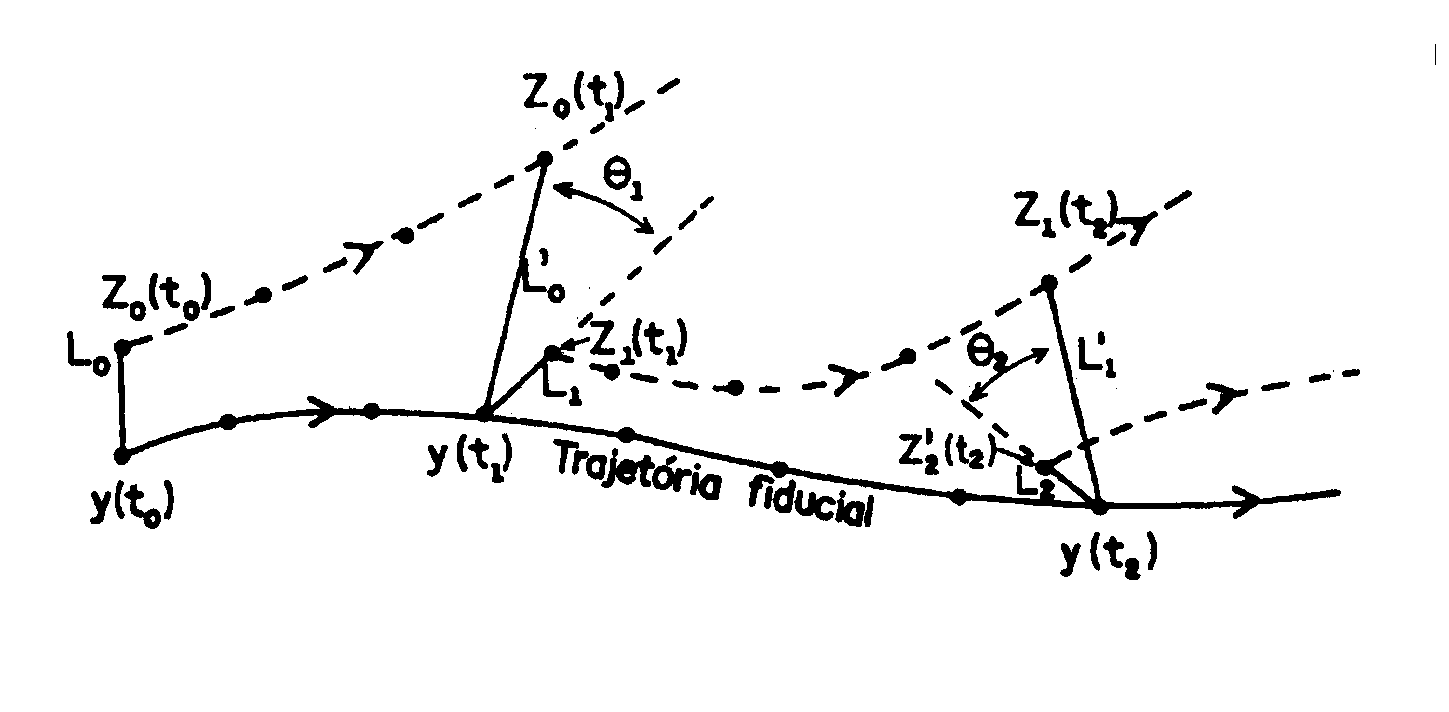
\includegraphics{Figuras/wolf.png}}
\caption{Representação esquemática do método proposto por \citeonline{wolf/85}. O maior expoente de Lyapunov é estimado a partir da taxa de crescimento dos segmentos $L_i$. Quando o comprimento do segmento que liga dois pontos próximos do atrator excede um certo valor $\epsilon$, um novo vizinho é escolhido de forma a minimizar o ângulo $\theta_i$.}
\FONTE{Adaptada de \citeonline{wolf/85}}
\label{figferraralyap}
\end{figure}

Através do método descrito acima é possível obter uma aproximação numérica para o maior expoente de Lyapunov, $\lambda_1$, calculado a partir da série temporal em $x$ de Lorenz. Pode-se observar que a aproximação obtida é satisfatória já que o maior expoente de Lyapunov, obtido diretamente do Sistema de EDO's (\ref{eqsistemalorenz}) é aproximadamente $2.16$ \cite{wolf/85}, enquanto que o obtido com base no algoritmo de \citeonline{wolf/85} é $2.18\pm0.01$.

\begin{figure}[ht]
\centering \resizebox{13cm}{!}{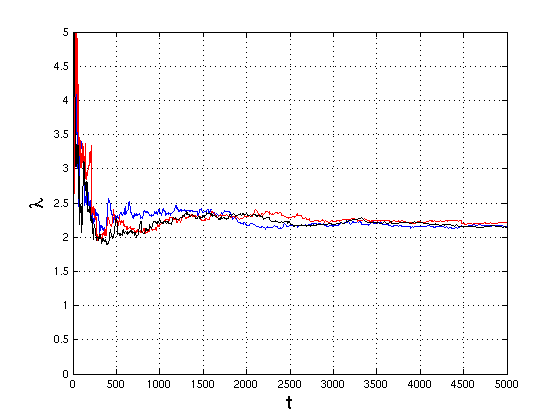
\includegraphics{Figuras/lorenzlyap3cond.png}}
\caption{Convergência do maior expoente de Lyapunov ($\lambda_1$) associado à componente $x$ do atrator de Lorenz, com base no algoritmo desenvolvido por \citeonline{wolf/85}. A curva azul corresponde à condição inicial $(5,5,5)$, a curva vermelha corresponde à condição inicial $(5.01,5,5)$ e a curva preta corresponde à condição inicial $(5,10,5)$}
\label{figlorenzlyap}
\end{figure}

\subsection{Plots de Recorrência}

A representação gráfica bidimensional de uma matriz da forma:

\begin{equation}
R_{i,j}=\Theta(\varepsilon-\|\xi_{i}-\xi_{j}\|),\;\;\; i,j=1,\ldots,M
\label{eqplotrec}
\end{equation}

é definida como \textit{Plots de Recorrência} (PR) e foi introduzida por \citeonline{eckmannplotrecorr/87}. Desta forma, $\xi_{i}\in\mathds{R}^m$ são vetores de dimensão $m$ obtidos através da reconstrução do espaço de fase (\ref{eqtakensreconst}), $\varepsilon$ é um valor limite pré-definido e $\Theta$ é uma função degrau de Heavyside (conforme~\ref{eqheavyside}). Se a distância entre dois vetores $\xi_{i}$ e $\xi_{j}$ sobre a trajetória reconstruída for menor que $\varepsilon$, a função de Heavyside $\Theta$ assume o valor $1$, e neste caso a posição $(i,j)$ da matriz~(\ref{eqplotrec}) é representada por um ponto preto, caso contrário tal posição é representada por um ponto branco~\cite{eckmannplotrecorr/87,thielromano/04,thielemuitos/02,gaocai/00}.

Segundo \citeonline{eckmannplotrecorr/87} por meio de um PR é possível visualizar o comportamento de trajetórias no espaço de fase~\cite{eckmannplotrecorr/87} e ainda um PR mostra todos os tempos no qual um estado de um sistema dinâmico se repete. A repetição de estados é uma propriedade fundamental de um sistema dinâmico determinístico, e é um comportamento típico em sistemas caóticos ou não-lineares~\cite{thieltese/04}. 

Tradicionalmente, a visualização de espaços de fase com dimensões maiores que $3$ é feita por meio de projeções em sub-espaços de dimensão $2$ ou $3$. Contudo, um PR permite investigar a evolução de trajetórias em um espaço de fase com dimensões elevadas por meio da representação bidimensional de suas repetições. 

A Figura~\ref{figrpsistemas} apresenta PRs para um sistema estocástico, um sistema periódico e um sistema determinístico caótico. PRs associados à sistemas estocásticos freqüentemente apresentam uma certa homogeneidade em relação à distribuição de seus pontos (conforme Figura~\ref{figrpsistemas}(a)). Sistemas que oscilam periódicamente apresentam estruturas de repetições periódicas cujas distâncias entre esses padrões periódicos correspondem ao período (conforme Figura~\ref{figrpsistemas}(b)). Sistemas dinâmicos caóticos possuem estruturas diagonais paralelas à diagonal principal (conforme Figura~\ref{figrpsistemas}(c)). Essas estruturas ocorrem quando um segmento da trajetória reconstruída é paralelo à outro segmento, ou seja, a trajetória visita a mesma região do espaço de fase em diferentes tempos. O comprimento de tais estruturas é proporcional à duração da evolução local comum entre os segmentos da trajetória~\cite{thieltese/04,gaocai/00}.

\begin{figure}[ht]
\centering 
\resizebox{7.2cm}{!}{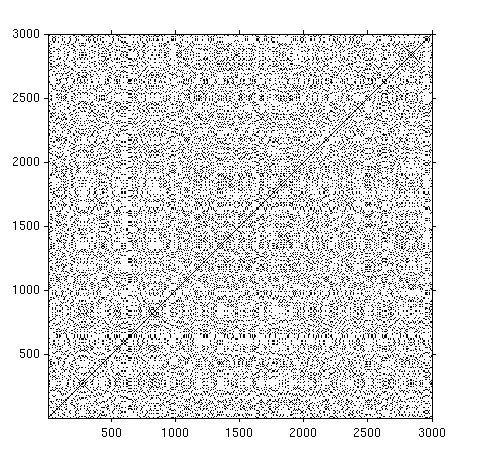
\includegraphics{Figuras/ruidorp.png}} \resizebox{7.2cm}{!}{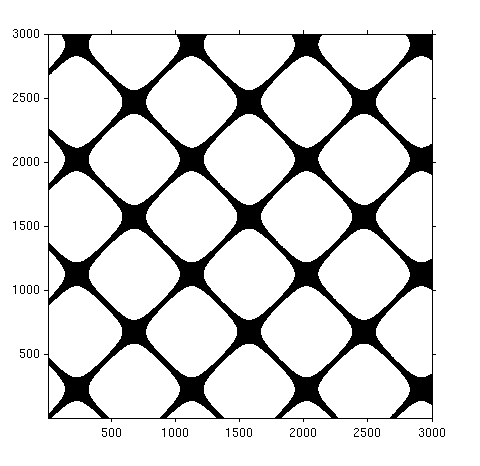
\includegraphics{Figuras/senorp.png}} \\  \resizebox{7.2cm}{!}{\includegraphics{Figuras/lorenzrp.png}} 
\caption{(a) PR para um sistema estocástico (ruído uniformemente distribuído) com $m=1$ e $\varepsilon=0.09994$ . (b) PR para a função seno com $m=1$ e $\varepsilon=0.2$. (c) PR correspondente à componente em $x$ do atrator de Lorenz com $m=6$ e $\varepsilon=4.9344$. O valor de $\varepsilon$ utilizados nos casos (a) e (b) correspondem à $10\%$ das variâncias associadas, e no caso (c) à $10\%$ do diâmetro do espaço de fase~\cite{thielromano/04}.}
\label{figrpsistemas}
\end{figure}

% \begin{figure}[ht]
% \centering 
% \resizebox{13cm}{!}{\includegraphics{Figuras/lorenzdet.png}\includegraphics{Figuras/lorenzembardet.png}}
% \caption{Atrator de Lorenz para o sistema~(\ref{eqsistemalorenzpart}). (a) Atrator original. (b) Atrator reconstruído pelo método das derivadas.}
% \label{lorenzdiff}
% \end{figure}

Uma das principais vantagens na aplicação de um PR, em comparação à aplicação de técnicas de caracterização de comportamento caótico tradicionais (como por exemplo o algoritmo de Grassberger e Procaccia~(\ref{eqcorr2})), é que o PR pode ser aplicado em séries temporais não estacionárias e com poucos pontos~\cite{thieltese/04}. Uma desvantagem é que se o número de pontos da série temporal for muito grande (maior que 10.000 pontos), o número de vetores reconstruídos é também grande. Conseqüentemente, a ordem da matriz de distâncias~(\ref{eqplotrec}) se torna elevada. Este fato pode acarretar em insuficiência de memória computacional na armazenagem desta matriz.



 %% 3o capítulo

%%%%%%%%%%%%%%%%%%%%%%%%%%%%%%%%%%%%%%%%%%%%%%%%%%%%%%%%%%%%%%%%%%%%%%%%%%%%%%%

\chapter{DADOS ANALISADOS}

Este capítulo aborda as características gerais da Região Amazônica. Apresenta-se a seguir a descrição e relevância do projeto LBA. Finalizando, é realizada a descrição dos dados coletados pela campanha WETAMC do projeto LBA, como também do sítio experimental, durante tal campanha.

\section{A Amazônia}
\label{sec:amazonia}

O bioma\footnote{Corresponde a certos padrões de clima, formações geológicas, relevo, solo, hidrografia, vegetação e biodiversidade, com características paisagísticas bem definidas.}Amazônia ocupa $50\%$ da superfície da América do Sul, toda a porção norte, distribuída por nove países. Essa região é limitada a oeste pela Cordilheira dos Andes (com elevações de até $6.000$ metros), ao norte pelo Planalto das Guianas (com picos montanhosos de até $3.000$ metros), ao sul pelo Planalto Central (com altitudes típicas de $1.200$ metros) e ao leste pelo Oceano Atlântico. Em território brasileiro está mais da metade dos $6,9$ milhões de quilômetros quadrados originalmente cobertos por floresta~\cite{fisch/98}. 

Segundo o IBGE, aproximadamente $60\%$ da Floresta Amazônica pertence ao território brasileiro, que compreende a Amazônia Legal\footnote{Em $1953$, a Constituição Federal criou o conceito político de ``Amazônia Legal'', que representa $61\%$ do território brasileiro. Além dos sete estados da região Norte, inclui o estado do Mato Grosso e cerca de $79\%$ do estado do Maranhão}. Os $40\%$ restantes estão distribuídos entre os países da Bolívia, Colômbia, Equador, Guiana, Guiana Francesa, Peru, Suriname e Venezuela. 

Parte da vegetação na Amazônia sofre grande influência do processo de subida e descida das águas, o chamado pulso hidrológico. As florestas inundáveis representam $5$ a $10\%$ da área da Amazônia. São definidas por estarem alagadas durante parte do tempo, diariamente, no caso dos manguezais, ou alguns meses por ano, no caso das várzeas e igapós, ou mesmo durante todo o ano, como nos pântanos. 

As florestas de terra firme representam mais de $80\%$ da área amazônica. Tais florestas estão livres de inundações, já que ocupam terras mais altas com altitudes médias de $200$ metros. Esse tipo de floresta apresenta árvores de grande porte, que variam de $30$ a $60$ metros em altura. O dossel retém cerca de $95\%$ dos raios solares, o que torna o interior da floresta úmido e escuro. 

A convecção na região amazônica é um importante mecanismo de aquecimento da atmosfera tropical e sua variação, em termos de intensidade e posição, possue um papel importante na determinação do tempo e do clima desta região~\cite{fisch/98}. O clima é, em geral, quente e úmido e o comportamento da temperatura do ar apresenta uma pequena variação ao longo do ano. A amplitude térmica sazonal é da ordem de $1$-$2\,^{\circ}$C, sendo que os valores médios situam-se entre $24\,^{\circ}$ e $28\,^{\circ}$C.

A precipitação é um dos elementos climáticos mais importantes a ser analisado na região tropical, pois induz as características e comportamento de variáveis tais como temperatura, umidade relativa, vento etc. A região amazônica possui uma precipitação média de aproximadamente $2.300$ mm.ano$^{-1}$. O período de chuvas ou forte atividade convectiva na região amazônica é compreendido entre novembro a março, sendo que o período de seca (sem grande atividade convectiva) ocorre entre os meses de maio e setembro. Os meses de abril e outubro são meses de transição entre um regime e outro~\cite{fisch/98}.

O conhecimento das diversas componentes envolvidas na interação entre a biosfera e a atmosfera é fundamental para a previsão da evolução do clima, da sustentabilidade do ecossistema como um todo, assim como para a tomada de decisão sobre as políticas públicas mais adequadas para a minimização de impactos danosos irreversíveis~\cite{silvadias/05}. 

 
\section{O projeto LBA}

Nas últimas décadas, vários experimentos micrometeorológicos têm sido realizados na região amazônica, com o objetivo de aumentar os conhecimentos relativos à interação entre a floresta tropical e a atmosfera. Dentre os experimentos realizados destaca-se a campanha micrometeorológica intensiva do Projeto LBA (Experimento de Grande Escala de Interação Biosfera-Atmosfera na Amazônia). 

O projeto LBA é um grande programa de pesquisas liderado pelo Brasil e com cooperação científica internacional, composto por mais de $130$ projetos de pesquisas (já executados ou em fase de execução), financiados por várias agências nacionais (como o MCT, o CNPQ, a FAPESP, a FINEP/PPG7, etc) e internacionais (com destaques para a NASA e a National Science Foundation, dos EUA, a Comissão Européia, o IAI - Instituto Interamericano de Pesquisas de Mudanças Globais, etc)~\cite{nobre/2005}. 

As duas questões centrais do LBA são: (i) como funciona a Amazônia, na forma de um sistema regional, com respeito aos ciclos da água, energia, carbono, gases do efeito estufa e nutrientes?; e (ii) como as mudanças de uso da terra e do clima podem afetar o funcionamento físico, químico e biológico dos ecossistemas amazônicos? Estas questões levam em conta que as mudanças climáticas e ambientais têm efeito sobre o uso sustentável dos recursos naturais e, de uma forma geral, sobre as populações. Deste modo, o LBA visa auxiliar na definição de critérios de uso sustentável da floresta e do solo da Amazônia~\cite{nobre/2005}. 

A Figura~\ref{mapalocal} apresenta um mapa esquemático com as áreas de pesquisa de campo do LBA. As áreas principais fazem parte de duas transeções ecofisiológicas e de usos da terra. As áreas secundárias de pesquisa serão estabelecidas em toda a Amazônia.

\begin{figure}[ht]
	\caption{Mapa esquemático com a localização das áreas de pesquisa de campo do projeto LBA.}
	\vspace{6mm}	% acrescentar o espaçamento vertical apropriado entre o título e a borda superior da figura
	\begin{center}
		\resizebox{10.5cm}{!}{\includegraphics{Figuras/mapalbacorr.png}}		
	\end{center}
	\vspace{4mm}	% acrescentar o espaçamento vertical apropriado entre a borda inferior da figura e a legenda ou a fonte quando não há legenda (o valor pode ser negativo para subir)
	\legenda{Longitude em grau em abscisse e latitude em grau em ordenada.}	% legenda - para deixar sem legenda usar comando \legenda{} (nunca deve-se comentar o comando \legenda)
	\label{mapalocal}
	\FONTE{\citeonline{lba/06}.}	% fonte consultada (elemento obrigatório, mesmo que seja produção do próprio autor)
\end{figure}

\section{Sítio experimental e dados}
 
Os dados utilizados neste trabalho foram obtidos através de uma campanha micrometeorológica intensiva, a saber, WETAMC (Campanha de Mesoescala Atmosférica na Estação Úmida) que é parte do projeto LBA. Esta campanha foi realizada entre os meses de janeiro e março de 1999, na Reserva Biológica do Jaru ($10\,^{\circ}$46'S, $61\,^{\circ}$56'W), um sítio de floresta densa de aproximadamente $270$ mil hectares, pertencente ao Instituto Brasileiro do Meio Ambiente e dos Recursos Naturais Renováveis - IBAMA. Tal reserva está situada aproximadamente à $80$ Km ao norte de Ji-Paraná e a $120$ m acima do nível do mar, no estado de Rondônia, Brasil (ver Figura~\ref{rondonia}).  

\begin{figure}[ht]
	\caption{Mapa com a localização da campanha realizada pelo Projeto LBA.}
	\vspace{6mm}	% acrescentar o espaçamento vertical apropriado entre o título e a borda superior da figura
	\begin{center}
		\resizebox{11.5cm}{!}{\includegraphics{Figuras/rondonia.pdf}}		
	\end{center}
		\vspace{2mm}	% acrescentar o espaçamento vertical apropriado entre a borda inferior da figura e a legenda ou a fonte quando não há legenda (o valor pode ser negativo para subir)
	\legenda{}	% legenda - para deixar sem legenda usar comando \legenda{} (nunca deve-se comentar o comando \legenda)
	\label{rondonia}
	\FONTE{\citeonline{iag/05}.}	% fonte consultada (elemento obrigatório, mesmo que seja produção do próprio autor)
\end{figure}

Uma estação meteorológica automática foi montada para medidas de resposta rápida de precipitação pluvial, temperatura do ar, umidade relativa do ar, velocidade e direção do vento, radiação solar incidente e de radiação de ondas longas emitida pela atmosfera e pela superfície, com médias coletadas em períodos de $30$ minutos, a uma freqüência de amostragem de $60$ Hz. Instrumentos como termômetros e anemômetros tridimensionais foram utilizados na área de floresta para medir tais variáveis meteorológicas e os fluxos de superfície (calor latente e calor sensível). 

As medidas foram feitas com o auxílio de uma torre micrometeorológica de alumínio de $66$ m de altura, simultaneamente em três diferentes alturas: Nível Superior ($66$ m - acima da copa); Nível Médio ($45$ m - no topo da copa); e Nível Inferior ($21$ m - abaixo da copa). 
A área onde tal torre foi construída está rodeada pela floresta amazônica de terra firme em um raio de pelo menos $800$ metros. As Figuras~\ref{torre} e \ref{figtorre} mostram, respectivamente, um desenho esquemático da torre e as vistas superior e inferior da mesma. Maiores informações do sítio experimental podem ser encontradas em \citeonline{culf/96}.

\begin{figure}[ht]
	\caption{Desenho esquemático da torre micrometeorológica do projeto LBA.}
	\vspace{6mm}	% acrescentar o espaçamento vertical apropriado entre o título e a borda superior da figura
	\begin{center}
		\resizebox{14cm}{!}{\includegraphics{Figuras/torredesenho.pdf}}		
	\end{center}
	\vspace{2mm}	% acrescentar o espaçamento vertical apropriado entre a borda inferior da figura e a legenda ou a fonte quando não há legenda (o valor pode ser negativo para subir)
	\legenda{}	% legenda - para deixar sem legenda usar comando \legenda{} (nunca deve-se comentar o comando \legenda)
	\label{torre}
	\FONTE{\citeonline{edtese/99}}.
\end{figure}

\begin{figure}[ht]
	\caption{Torre micrometeorológica de $66$ metros de altura construída na Reserva Biológica do Jaru (Rebio-Jaru), em Rondônia.}
	\vspace{6mm}	% acrescentar o espaçamento vertical apropriado entre o título e a borda superior da figura
	\begin{center}
		\resizebox{10.5cm}{!}{\includegraphics{Figuras/2torres.pdf}}		
	\end{center}
	\vspace{2mm}	% acrescentar o espaçamento vertical apropriado entre a borda inferior da figura e a legenda ou a fonte quando não há legenda (o valor pode ser negativo para subir)
	\legenda{À esquerda, vista superior; à direita, vista inferior.}	% legenda - para deixar sem legenda usar comando \legenda{} (nunca deve-se comentar o comando \legenda)
	\FONTE{\citeonline{iag/05}}.
	\label{figtorre}
\end{figure}

Dois períodos de medidas distintos foram selecionados: às 12 horas, quando a copa da floresta é aquecida pelo sol e o topo da mesma é mais quente que os arredores, e desta forma a região acima da copa é instável; e às 23 horas, quando as condições são opostas, e a região acima da copa é estável~\cite{Ramos/04}. Durante o experimento, o estado da atmosfera foi caracterizado pela existência de uma forte atividade convectiva no período diurno, com eventos de chuvas isoladas de dia e à noite.

É importante destacar que os dados obtidos através desta campanha foram submetidos a um rigoroso controle de qualidade conforme \citeonline{bolzan/00}. Desta forma, problemas freqüentemente encontrados em sinais experimentais, como por exemplo picos espúrios e vales, foram removidos dos mesmos.
 %% 4o capítulo

%%%%%%%%%%%%%%%%%%%%%%%%%%%%%%%%%%%%%%%%%%%%%%%%%%%%%%%%%%%%%%%%%%%%%%%%%%%%%%%

\chapter{ANÁLISE E RESULTADOS}
\label{capanaliseseresults}

A possível natureza caótica da turbulência na camada limite atmosférica, no interior e acima da copa da floresta é investigada. Com base na aplicação de diversas ferramentas
%(já descritas no Capítulo~\ref{caputiltecnicas}) 
nas séries temporais em estudo, o objetivo deste trabalho é determinar se tais séries incluem componentes determinísticas que podem ser descritas (individualmente) por um sistema dinâmico de baixa dimensão, que se desenvolve em um atrator caótico.


\section{Estacionaridade}
Primeiramente, as séries temporais em estudo foram submetidas ao teste de estacionaridade.
% já descrito na Seção~\ref{subsecestacio}. 
A Tabela~\ref{tabelatempestacionaria} apresenta a classificação destas séries em estacionárias ou não estacionárias. Neste teste foram utilizadas janelas de dados deslizantes variáveis, a saber, $L=100,500$ e $1000$. Desta forma, as análises subseqüentes serão feitas apenas com as séries do tipo estacionárias.

\begin{table}[!ht]
\begin{center}
\caption{Análise da estacionaridade para as séries temporais de temperatura e velocidade do vento em diferentes períodos do dia e níveis da copa.}
\begin{tabular}{c c c}
\hline 
\textbf{Série temporal} & \textbf{Estacionaridade} \\
\hline
tS1200 & estacionária \\
tI1200 & estacionária \\
tS2300 & não-estacionária \\
tI2300 & estacionária \\
tM1200 & estacionária \\
wS1200 & estacionária \\
tM2300 & não-estacionária \\
\hline
\end{tabular}
\label{tabelatempestacionaria}
\end{center}
\end{table}

\section{Decomposição dos Dados}

Com o objetivo de investigar o papel das estruturas coerentes na existência (ou não) de caos na atmosfera, decidiu-se selecionar dentre o conjunto de séries disponíveis uma que apresentasse sinais nítidos da presença de estruturas coerentes em rampa e em seguida decompor a mesma (denominada de série total) em duas partes: uma parte dita coerente (baixas freqüências) e uma parte incoerente (altas freqüências). A parte coerente é caracterizada apenas pelas estruturas coerentes em rampa presentes na série total, enquanto que a parte incoerente é caracterizada pelas flutuações aparentemente aleatórias da mesma série. 

%\subsection{Decomposição dos dados}

Inicialmente, a série temporal total (tS1200) foi decomposta em suas partes coerente e incoerente, por meio da filtragem com Wavelet de Haar~\cite{katul/94}, que é um tipo de ondeleta-mãe discreta, definida por

\begin{equation}
\left\{ \begin{array}{rrr} 1, &  & 0\leq t < 1/2 \\
                  -1, &  & 1/2\leq t < 1 \\
		   0, &  & \mbox{caso contrário}
\end{array} 
\right.
\label{eqwavelethaar}
\end{equation} 

Esta categoria de ondaletas é utilizada para detectar variações bruscas nos sinais, e trabalha com sinais temporais que tenham comprimentos da ordem da potência de dois mais próxima, ou seja, $2^{f}=s$, onde $s$ é o comprimento total da série, e $f$ é o número de freqüências possíveis para a decomposição. 

O comprimento da série em estudo é de $s=108.000$ pontos. Desta forma, não há um número exato de decomposições em freqüências, já que $f=16$ resulta em $s=65.536$ pontos e $f=17$ resulta em $s=131.072$ pontos. A estratégia utilizada foi completar o início da série temporal com zeros até que a freqüência $f=17$ fosse alcançada. 
 
Ainda não há na literatura um consenso de qual seja a melhor função ondeleta a ser utilizada para a decomposição e filtragem de uma série temporal. O que comumente se aceita é que a função ondeleta possua um formato característico próximo das características encontradas na série temporal. Isso explica o fato da Wavelet de Haar ter sido escolhida para a decomposição da série temporal de temperatura.  

A Figura~\ref{figfiltrotS0681200} mostra a série temporal total, a série temporal coerente (soma das baixas freqüências da série total) e a série temporal incoerente (soma das altas freqüências da série total), respectivamente. Após a filtragem da série total, $23072$ pontos iniciais foram descartados das séries total, coerente e incoerente; tal valor corresponde ao número de zeros inseridos na série total antes do procedimento de filtragem. É importante ressaltar que a soma da série coerente com a série incoerente resulta a série total, o que já era esperado.

\begin{figure}[ht]
	\caption{Séries temporal total, coerente e incoerente.}
	\vspace{0mm}	% acrescentar o espaçamento vertical apropriado entre o título e a borda superior da figura
	\begin{center}
		\resizebox{13cm}{!}{\includegraphics{Figuras2/filtrocoltS0681200.png}}		
	\end{center}
	\vspace{-2mm}	% acrescentar o espaçamento vertical apropriado entre a borda inferior da figura e a legenda ou a fonte quando não há legenda (o valor pode ser negativo para subir)
	\legenda{Sinal total (superior), soma das nove primeiras freqüências (meio), soma das sete últimas freqüências (inferior).}	% legenda - para deixar sem legenda usar comando \legenda{} (nunca deve-se comentar o comando \legenda)
	\label{figfiltrotS0681200}
	\FONTE{Produção do autor.}	% fonte consultada (elemento obrigatório, mesmo que seja produção do próprio autor)
\end{figure}

\section{Caracterizando a turbulência acima da copa da floresta Amazônica}

O objetivo desta seção é verificar se as séries total, coerente e incoerente possuem as características típicas da turbulência plenamente desenvolvida, a saber, espectros de potência do tipo Kolmogorov e intermitência nas pequenas escalas. Aproveita-se para ilustrar o papel crucial das estruturas coerentes no transporte de propriedades (quantidade de movimento, calor, etc.) através da copa da floresta.

\subsection{Espectros de potência}

Os espectros de potência das séries temporais total, coerente e incoerente foram estimados usando FFT (ver Figura~\ref{figespectrotS0681200}). Os resultados mostram que as inclinações desses espectros no SI (em escala $\log$-$\log$) coincidem com a lei dos $-5/3$ de Kolmogorov. Esta observação demonstra que o fenômeno da turbulência está presente na série total, o que era esperado, mas também nas séries coerente e incoerente. Em especial, pode-se afirmar que a série incoerente está mais relacionada à turbulência de pequena escala do que a algum tipo de ruído. Este comportamento é consistente com outros estudos que utilizaram a mesma abordagem de separação de um fluxo turbulento em uma parte coerente e outra incoerente~\cite{farge/01}.

\begin{figure}[ht]
	\caption{Espectros de potência das séries temporais total, coerente e incoerente.}
	\vspace{0mm}	% acrescentar o espaçamento vertical apropriado entre o título e a borda superior da figura
	\begin{center}
		\resizebox{15cm}{!}{\includegraphics{Figuras2/tS0681200espectro.png}\includegraphics{Figuras2/ctS0681200espectro.png}}\\ \resizebox{7.5cm}{!}{\includegraphics{Figuras2/itS0681200espectro.png}}		
	\end{center}
	\vspace{2mm}	% acrescentar o espaçamento vertical apropriado entre a borda inferior da figura e a legenda ou a fonte quando não há legenda (o valor pode ser negativo para subir)
	\legenda{Em azul espectro de potência da série temporal total, em vermelho da série temporal coerente e em rosa da série temporal incoerente. Observe que as inclinações de todos os espectros no SI (em escala $\log$-$\log$) coincidem com a lei dos $-5/3$ de Kolmogorov. O espectro de potência associado a série incoerente possui uma inclinação adicional de $2.7$, que pode estar associada a um artefato numérico.}	% legenda - para deixar sem legenda usar comando \legenda{} (nunca deve-se comentar o comando \legenda)
	\label{figespectrotS0681200}
	\FONTE{Produção do autor.}	% fonte consultada (elemento obrigatório, mesmo que seja produção do próprio autor)
\end{figure}

\subsection{Intermitência}

A detecção do fenômeno intermitente foi feita a partir das diferenças das séries de temperatura total, coerente e incoerente (medida às $12$ horas no nível superior) em várias escalas $r_{i}$ com $i=1,\ldots4$. Desta forma, as FDP's foram obtidas com base na distribuição estatística das diferenças $\Delta T_{r_{i}}=T(x+\Delta r_{i})-T(x)$. Os valores assumidos por $\Delta r_{i}$ são dados respectivamente por $1,10,100$ e $1000$, que para dados amostrados à $60$ Hz correspondem a $\Delta T_{t_{i}}$ de aproximadamente $0.0167,0.1667,1.6667$ e $16.6667$ segundos, respectivamente. %% 5o capítulo

%%%%%%%%%%%%%%%%%%%%%%%%%%%%%%%%%%%%%%%%%%%%%%%%%%%%%%%%%%%%%%%%%%%%%%%%%%%%%%%

\chapter{CONCLUSÕES}


Neste trabalho foi analisada a possível natureza caótica da turbulência atmosférica. Trata-se de uma questão ainda em aberto para a qual existem resultados discrepantes. As análises aqui realizadas, baseadas em dados de temperatura de alta resolução, obtidos pela campanha WETAMC do projeto LBA, sugerem a existência de um comportamento caótico de baixa dimensão na camada limite atmosférica. O atrator caótico correspondente possui uma dimensão de correlação de $D_{2}=3.50\pm0.05$. A presença de dinâmica caótica nos dados analisados é confirmada com a estimativa de um expoente de Lyapunov pequeno mas positivo, com valor $\lambda_{1}=0.050\pm0.002$. No entanto, esta dinâmica caótica de baixa dimensão está associada à presença das estruturas coerentes na camada limite atmosférica e não à turbulência atmosférica, como anteriormente afirmado por vários autores~\cite{xin/01,jaramillo/93,gallego/01}. Esta afirmação é evidenciada pelo processo de filtragem por wavelets utilizado nos dados experimentais estudados, que permite separar a contribuição da estruturas coerentes do sinal turbulento de fundo.

Este resultado corrobora a conjectura de \citeonline{loratrat/91}, que afirma que as ligações existentes entre caos e clima, apresentadas na literatura, decorrem não de erros de análise, mas da existência de subsistemas caóticos de baixa dimensão fracamente acoplados a um sistema maior, mais complexo e não caótico. No contexto deste trabalho, os subsistemas de baixa dimensão seriam as estruturas coerentes, comumente encontradas na camada limite, e o sistema maior, a atmosfera complexa e turbulenta. Os resultados obtidos neste trabalho, tanto para a dimensão de correlação $D_{2}$ quanto para o expoente de Lyapunov $\lambda_{1}$, são consistentes com valores publicados na literatura, onde evidências de atratores de baixa dimensão na atmosfera foram detectados~\cite{xin/01,jaramillo/93,gallego/01}. Apesar da presença de estruturas coerentes não ser explicitamente mencionada nestes trabalhos, uma leitura cuidadosa dos mesmos fornece indícios de que as séries temporais estudadas por esses autores possuem estruturas do tipo rampa, como as analisadas neste trabalho.
 
No plano computacional, esta dissertação ofereceu a oportunidade de estudar e implementar diversas ferramentas para o estudo de comportamento caótico em séries temporais. Apesar de populares, a maior parte destes algoritmos apresenta sérias dificuldades quando confrontados com o desafio de analisar séries ``reais'' (isto é, oriundas de sistemas dinâmicos naturais não conhecidos a priori), fracamente estacionárias, com muitos pontos (100 mil ou mais) e ainda por cima, contaminadas com ruído. Neste sentido, um resultado importante desta dissertação foi o desenvolvimento de uma ``cultura'' local, composta por adaptações, truques, etc., que permitiu ir além dos dados sintéticos e utilizar este tipo de série temporal. Esta ``cultura'' normalmente
permanece invisível na hora de relatar os resultados obtidos em uma pesquisa, mas é de fundamental importância para a realização de trabalhos futuros na área.

Finalmente, como linhas de pesquisa para trabalhos futuros sugere-se o desenvolvimento de um modelo dinâmico mínimo para descrever o comportamente das estruturas coerentes na copa da floresta, sob condições convectivas. Um modelo do tipo instabilidade de Kelvin-Helmholtz, que reconhecidamente apresenta propriedades caóticas~\cite{malik/92}, seria um bom ponto de partida. A análise de mais séries turbulentas que apresentem uma estrutura do tipo rampa, sob diferentes condições experimentais, é também uma continuação natural deste trabalho. %% 6o capítulo


%% insira quantos capítulos desejar com o seguinte comando:
%\include{_pasta_do_arquivo_/_meu_arquivo_} %%sem a extensão
%% note que deverá haver um arquivo _meu_arquivo_.tex (com extensão) no diretório _pasta_do_arquivo_

%\include{./docs/conclusao}

%% Bibliografia %% não alterar %% obrigatório %testebib
\bibliography{./bib/referencia} %% aponte para seu arquivo de bibliografia no formato bibtex (p.ex: referencia.bib)


%\include{./docs/glossario} %% insira os termos do glossário no arquivo glossario.tex %% opcional

\inicioApendice %% opcional, comente esta linha e a seguintes se não houver apendice(s)
%%%%%%%%%%%%%%%%%%%%%%%%%%%%%%%%%%%%%%%%%%%%%%%%%%%%%%
%Apêndice A
\hypertarget{estilo:apendice1}{} %% uso para este Guia
%Este apêndice foi criado apenas para indicar como construir um apêndice no estilo, não existia no original da tese.
%%%%%%%%%%%%%%%%%%%%%%%%%%%%%%%%%%%%%%%%%%%%%%%%%%%%%%
\renewcommand{\thechapter}{}%
\chapter{APÊNDICE A - AUTORIZAÇÃO PARA PUBLICAÇÃO}	% trocar A por B na próxima apêndice e etc
\label{apendiceA}	% trocar A por B na próxima apêndice e etc
\renewcommand{\thechapter}{A}%		% trocar A por B na próxima apêndice e etc

Há dois formulários de autorização para publicação, um para publicações de trabalhos acadêmicos e outro para publicações técnico-científicas, neste apêndice encontram-se os modelos dos formulários e suas respectivas instruções de preenchimento. 

\section{Autorização para Publicação de Trabalho Acadêmico - INPE-393}

\label{instr393}

	\begin{figure}[ht]
		\caption{Formulário Autorização para Publicação de Trabalho Acadêmico INPE-393.}
		\vspace{6mm}	% acrescentar o espaçamento vertical apropriado entre o título e a borda superior da figura
		\centering
   		\includegraphics[height=16cm]{./Figuras/form393.png}	   
 		\label{form393}
	\end{figure}


\subsection{Instruções do Formulário INPE-393} 

\begin{enumerate} 

 \item \textbf{série:} com este número o SID identifica as publicações do INPE, composto da sigla da Instituição, número sequencial geral da publicação, sigla e número sequencial do tipo de publicação, exemplo: INPE-14209-TDI/1110;
 
 \item \textbf{número:} será composto da sigla da unidade do SID, mais 4 (quatro) dígitos e do ano em curso. Este número de referência é de controle da unidade emissora. Ex.: SID-0001/2007;

 \item \textbf{título da publicação:} deve ser completo, evitando-se abreviar palavras;

 \item \textbf{nome do autor e do orientador:} estes campos devem ser preenchidos por extenso, da mesma forma em que irão constar da publicação;

 \item \textbf{origem da publicação:} sigla da unidade do servidor (autor da publicação), conforme TQ-001;

 \item \textbf{curso:} sigla do curso, de acordo com a Estrutura de Divisão de Trabalho - EDT do INPE;
 
 \item \textbf{tipo:} assinalar se é tese ou dissertação;

 \item \textbf{apresentação:} colocar a data de aprovação final;

 \item \textbf{revisão técnica:} o responsável designado pela Banca Examinadora para verificação de correções e, na ausência desse, o orientador da tese ou dissertação deve
carimbar, datar e assinar após a versão \emph{on line} do trabalho;

 \item \textbf{revisão de linguagem:} o responsável designado pela Banca Examinadora para verificação de correções, e na ausência deste o orientador deve assinalar a solicitação ou a dispensa da revisão de linguagem e, carimbar, datar e assinar; o revisor deve datar e assinar após a revisão;
 
 \item \textbf{distribuição:} O SID deve informar a quantidade de CD's e de cópias impressas da tese ou dissertação, conforme lista de distribuição;
 
 \item \textbf{verificação de normalização:}  Após a verificação da versão \emph{on line} do trabalho quanto às normas editoriais, o SID deve datar e assinar;
 
 \item \textbf{autorização final:} data e assinatura do Titular de Nível A, conforme TQ-001, a que o Serviço de Pós-Graduação estiver subordinado.
 
 \item \textbf{observações:} para outras informações necessárias. 

\end{enumerate}

\section{Autorização para Publicação - INPE-106}
\begin{figure}[ht!]
	\caption{Formulário Autorização para Publicação de Trabalho Acadêmico INPE-106 folha 1.} 
	\vspace{6mm}	% acrescentar o espaçamento vertical apropriado entre o título e a borda superior da figura
	\centering
	\includegraphics[height=18cm]{./Figuras/form106.png}
	\label{form106}
\end{figure}

\begin{figure}[ht!]
	\caption{Formulário Autorização para Publicação de Trabalho Acadêmico INPE-106 folha 2.} 
	\vspace{6mm}	% acrescentar o espaçamento vertical apropriado entre o título e a borda superior da figura
	\centering
	\includegraphics[height=18cm]{./Figuras/form106folha2.png}
	\label{form106a}
\end{figure}

\clearpage
\subsection{Instruções do Formulário INPE-106} 
\label{instr106}


\begin{enumerate}

 \item \textbf{série:} com este número o SID identifica as publicações do INPE, composto da sigla da Instituição, número sequencial geral da publicação, sigla e número sequencial do tipo de publicação, exemplo: INPE-5616-RPQ/671. 
 
 \item \textbf{número:} será composto da sigla da unidade constante da Estrutura Organizacional do INPE (TQ-001), mais 4 (quatro) dígitos e do ano em curso. Este número de referência é de controle da unidade solicitante. Ex: CEA-0001/2007;
 
 \item \textbf{título da publicação:} deve ser completo, evitando-se abreviar palavras;

 \item \textbf{nome do autor, tradutor e editor:}  estes campos devem ser preenchidos por extenso, da mesma forma em que irão constar da publicação;

 \item \textbf{origem da publicação:} sigla da unidade do servidor (autor da publicação), conforme TQ-001;

 \item \textbf{projeto:} sigla do projeto de acordo com a Estrutura de Divisão de Trabalho - EDT do INPE;

 \item \textbf{tipo de publicação:} assinalar o tipo de publicação proposta:

 \begin{enumerate}
  \item{Relátorio de Pesquisa (RPQ)},
  \item{Notas Técnico-Científicas (NTC)},
  \item{Propostas e Relatórios de de Projeto (PRP)},
  \item{Manuais Técnicos (MAN)},
  \item{Publicações Didáticas (PUD)},
  \item{Trabalhos Acadêmicos Externos (TAE)}.
 \end{enumerate}

 \item \textbf{divulgação:} assinalar, de acordo com os critérios de classificação. Se houver Lista de Divulgação, nesta deverá constar os nomes e endereços completos;

 \item \textbf{convênio:} descrever o nome da instituição, quando a publicação for realizada pelo INPE e outra organização, preencher somente para o tipo PRP; 
 
    \item \textbf{autorização preliminar:} data, carimbo e assinatura do Titular da Unidade a que o autor esteja subordinado e, assinatura do revisor que efetuou a revisão técnica aprovando a versão \emph{on line} do trabalho e do revisor que realizou a revisão de linguagem, quando solicitadas; 
    
  \item \textbf{verificação de normalização:} o SID deve datar e assinar após a revisão da adequação às normas editoriais;   
  
  \item \textbf{distribuição:} O SID deve informar a quantidade de CD's e de cópias impressas que deverão ser gravados conforme lista de distribuição;
  
 \item \textbf{autorização final:} data, carimbo e assinatura do Titular de Nível "A", conforme TQ-001, a que o autor da publicação estiver subordinado;
 
 \item \textbf{observações:} para outras informações necessárias, inclusive para descrever as justificativas de uma publicação.
\end{enumerate} %% insira apendices tal qual capítulos acima


\inicioAnexo
%%%%%%%%%%%%%%%%%%%%%%%%%%%%%%%%%%%%%%%%%%%%%%%%%%%%%%
%Anexo
%Este anexo foi incluido para explicar como incluir um anexo no estilo, não existia no original desta tese.
%%%%%%%%%%%%%%%%%%%%%%%%%%%%%%%%%%%%%%%%%%%%%%%%%%%%%%%%%%%%%%%%%%%%%%%%%%%%%%%%%
\renewcommand{\thechapter}{}%
\chapter{ANEXO A - ABREVIATURA DOS MESES} %% Título do anexo sempre em maiúsculas. Trocar A por B no próximo anexo e etc
\label{anexoA} %% Rótulo aplicado caso queira referir-se a este tópico em qualquer lugar do texto. Trocar A por B no próximo anexo e etc
\renewcommand{\thechapter}{A}%		% trocar A por B no próximo anexo e etc

\begin{table}[!ht]
 \label{tab:abreviaturas}
  \begin{center}
 	\begin{tabular}{lll}
	 \hline
	  \textbf{Português}    & \textbf{Espanhol}  & \textbf{Italiano}\\ 
   \hline
       janeiro   = jan.   & enero = ene.       & gennaio = gen.\\
       fevereiro = fev.   & febrero = feb.     & febbraio = feb.\\
       março     = mar.   & marzo = mar.       & marzo = mar.\\
       abril     = abr.   & abril = abr.       & aprile = apr.\\
       maio      = maio   & mayo = mayo        & maggio = mag.\\ 
       junho     = jun.   & junio = jun.       & giugno = giu.\\ 
       julho     = jul.   & julio = jul.       & luglio = lug.\\
       agosto    = ago.   & agosto = ago.      & agosto = ago.\\
       setembro  = set.   & septiembre = sep.  & settembre = set.\\
       outubro   = out.   & octubre = oct.     & ottobre = ott.\\
       novembro  = nov.   & noviembre =nov.    & novembre = nov.\\
       dezembro  = dez.   & diciembre = dic.   & dicembre = dic.\\ 
     \hline
   \textbf{Francês}       & \textbf{Inglês}    & \textbf{Alemão}\\
     \hline
       janvier = jan.     & January = Jan.     & Januar = Jan.\\
       février = fév.     & February = Feb.    & Februar = Feb.\\
       mars = mars        & March = Mar.       & März = März\\
       avril = avr.       & April = Apr.       & April = Apr.\\
       mai = mai          & May = May          & Mai = Mai.\\
       juin = juin        & June = June        & Juni = Juni\\
       juillet = juil.    & July = July        & Juli = Juli\\
       août = août        & August = Aug.      & August = Aug.\\
       septembre = sept.  & September = Sept.  & September = Sept.\\
       octobre = oct.     & October = Oct.     & Oktober = Okt.\\
       novembre = nov.    & November = Nov.    & November = Nov.\\
       décembre = déc.    & December = Dec.    & Dezember = Dez. \\ 
    \hline
   \end{tabular}
   \end{center}
	 \FONTE{Adaptada de \citeonline[p.~22]{NBR6023:2002b}.}
\end{table}
%%%%%%%%%%%%%%%%%%%%%%%%%%%%%%%%%%%%%%%%%%%%%%%%%%%%%%%
%Anexo
%Este anexo foi incluido para explicar como incluir um anexo no estilo, não existia no original desta tese
%exceto algumas tabelas que foram modificadas
%%%%%%%%%%%%%%%%%%%%%%%%%%%%%%%%%%%%%%%%%%%%%%%%%%%%%%%%%%%%%%%%%%%%%%%%%%%%%%%%%
\renewcommand{\thechapter}{}%
\chapter{ANEXO B - EXEMPLOS DE FIGURAS E TABELAS NO \LaTeX} %% Título do anexo sempre em maiúsculas.
\label{anexoB} %% Rótulo aplicado caso queira referir-se a este tópico em qualquer lugar do texto.
\renewcommand{\thechapter}{B}%

\section{Figuras} %% Título de secção sempre com as primeiras letras em maiúsculas.
\label{anexo2}

\begin{figure}[ht]
	\caption{Exemplo de figura com título curto.}
	\vspace{6mm}	% acrescentar o espaçamento vertical apropriado entre o título e a borda superior da figura
	\begin{center}
    	\includegraphics[width=\mylenfig]{./Figuras2/gpa.pdf}  
	\end{center}
	\vspace{4mm}	% acrescentar o espaçamento vertical apropriado entre a borda inferior da figura e a legenda ou a fonte quando não há legenda (o valor pode ser negativo para subir)
	\legenda{Exemplo de legenda curta.}	% legenda - opcional
	\label{figgpa1}
	\FONTE{\citeonline{lba/06}.}	% fonte consultada (elemento obrigatório, mesmo que seja produção do próprio autor)
\end{figure}

\begin{figure}[!h]
	\caption{Figura com título que ocupa mais de uma linha, alinhar as demais com a primeira
letra depois do hífen.}
%o ajuste do título é feito automaticamente pelo \LaTeX\ caso este ocupe mais de uma linha.}
	\vspace{6mm}	% acrescentar o espaçamento vertical apropriado entre o título e a borda superior da figura
	\begin{center}
    	\includegraphics[width=\mylenfig]{./Figuras2/gpa.pdf}  
	\end{center}
	\vspace{4mm}	% acrescentar o espaçamento vertical apropriado entre a borda inferior da figura e a legenda ou a fonte quando não há legenda (o valor pode ser negativo para subir)
	\legenda{Exemplo de legenda que ocupa mais de uma linha, alinhar as demais com a primeira
letra da primeira linha.}	% legenda - opcional
%o \LaTeX\ alinha o texto automaticamente.
	\label{figgpa2}
	\FONTE{Se o texto da fonte for longo e ocupar mais de uma linha as demais ficam alinhadas
	com a palavra fonte. Adaptada de \citeonline{mauri:2003}.}	% fonte consultada (elemento obrigatório, mesmo que seja produção do próprio autor)
%o \LaTeX\ alinha o texto automaticamente.
\end{figure}

\clearpage
\section{Tabelas} 

\begin{table}[!ht]%[htbp] %opções de colocação da tabela no texto
  \begin{center}	% use sempre um ambiente para as tabelas
									% (opções: center (recomendado), flushright, flushleft)
									% NÃO USE \centering com TABELAS se houver \FONTE!	
  \caption{Exemplo de tabela, com fonte.}
    \begin{tabular}{l|l|c|c|r|r}
			\hline % desenha uma linha horizontal
				Campo 1 & Campo2 & Campo3 & Campo 4 & Campo5 & Campo6 \\
				Campo 1 & Campo2 & Campo3 & Campo 4 & Campo5 & Campo6 \\
				Campo 1 & Campo2 & Campo3 & Campo 4 & Campo5 & Campo6 \\				
			\hline % desenha uma linha horizontal
    \end{tabular}
    \end{center}
 \FONTE{Coloque a fonte de referência aqui, se houver.}
\end{table}

% \hhline{|--|} \multicolumn{2}{|c|}{continuação da página anterior} \\
% \hhline{|--|} \endhead % ate aqui eh definicao do "head" da pagina 
%   % dois em diante
% \hhline{|--|} \multicolumn{2}{|c|}{continua para próxima página} \\
% \hhline{|--|} \endfoot % ate aqui eh definicao do "foot" exceto ultima página
% \hhline{|b:=:=:b|} \endlastfoot % ate aqui eh definicao do "foot" 
%   % da ultima pagina

\begin{table}[hb]
\renewcommand{\baselinestretch}{1.4}% for tabular environment
\small
   \centering
   \caption{Exemplo de tabela, com fonte longa}
%   \label{\fullpaperid:table:1}% you must prefix your labels (here table:1) with the string \fullpaperid: (this will be important when combining all the full papers for the final book)
	\begin{center}
	   \begin{tabular}{lcc}
	       \hline% horizontal line
	       \itshape Parameter&
	           \itshape $\kappa$ Scaling&
	           \itshape $\kappa$, $\lambda$ Scaling\\*
	       \hline
	       Dimension&
	           $\kappa^{-1}$&
	           $\lambda^{-1}$\\*
	       Currant&
	           $\kappa^{-1}$&
	               $\lambda/\kappa^{2}$\\*
	       Dopant Concentration&
	           $\kappa$&
	           $\lambda2/\kappa$\\*
	       \hline
	   \end{tabular}
	\end{center}
    \renewcommand{\baselinestretch}{1.0}
    \FONTE{Coloque a fonte longa longa longa longa longa longa longa longa longa longa aqui, se houver.}
\end{table}

% Exemplos de 2 tabelas avançadas 

\begin{table}[ht!]
\caption{Outro exemplo de tabela}
%\label{\fullpaperid:table:2}
\begin{center}
\renewcommand{\baselinestretch}{1.2}% for tabular environment
\small
\begin{tabular}{cccccc}
\hline
   & \multirow{2}{22mm}{\renewcommand{\baselinestretch}{0.7}\small\centering Quantitative measures} & \multicolumn{4}{c}{Markers} \\ \cline{3-6}
   & & \multicolumn{1}{c}{RO} & \multicolumn{1}{c}{ASF} & \multicolumn{1}{c}{ISO} & \multicolumn{1}{c}{ADF} \\ \hline
   \multirow{3}{20mm}{\renewcommand{\baselinestretch}{0.7}\small\centering Test image scale 2}
& RMSE & 0.126 & 0.187 & 0.118 & 0.103 \\
& NMSE & 0.046 & 0.101 & 0.040 & 0.031 \\
& SSIM & 0.9981 & 0.9956 & 0.9984 & 0.9989 \\ \hline
   \multirow{3}{18mm}{\renewcommand{\baselinestretch}{0.7}\small\centering Cameraman scale 4}
& RMSE & 13.748 & 15.649 & 10.132 & 4.325 \\
& NMSE & 0.011 & 0.014 & 0.006 & 0.001 \\
& SSIM & 0.923 & 0.847 & 0.904 & 0.933 \\ \hline
   \multirow{3}{18mm}{\renewcommand{\baselinestretch}{0.7}\small\centering Cameraman scale 7}
& RMSE & 20.963 & 22.652 & 13.108 & 4.650 \\
& NMSE & 0.024 & 0.029 & 0.010 & 0.001 \\
& SSIM & 0.851 & 0.757 & 0.866 & 0.925 \\ \hline
   \multirow{3}{23mm}{\renewcommand{\baselinestretch}{1.2}\small\centering Crop of cameraman scale 7}
& RMSE & 30.914 & 31.943 & 17.831 & 2.870 \\
& NMSE & 0.053 & 0.057 & 0.018 & 0.001 \\
& SSIM & 0.831 & 0.772 & 0.891 & 0.983 \\ \hline
\end{tabular}
\end{center}
\end{table}

\begin{table}[ht!]
\caption{Mais um exemplo de tabela}
%\label{\fullpaperid:table:1}
\begin{center}
\renewcommand{\baselinestretch}{1.2}% for tabular environment
\small
\begin{tabular}{ccccc}
\hline
\multirow{4}{16mm}{\renewcommand{\baselinestretch}{0.7}\small\centering Leveling's Scale} & \multicolumn{4}{c}{Values for the scale relation of the four different type of markers} \\ \cline{2-5}
& \multirow{3}{29mm}{\renewcommand{\baselinestretch}{1}\small\centering Structure element's size $r$ for RO and ASF} & \multicolumn{2}{c}{Isotropic diffusion} & \multirow{3}{20mm}{\renewcommand{\baselinestretch}{1}\small\centering Anisotropic diffusion iterations $t$} \\ \cline{3-4}
& & \multirow{2}{23mm}{\renewcommand{\baselinestretch}{0.7}\small\centering Standard deviation $\sigma$} & \multirow{2}{12mm}{\renewcommand{\baselinestretch}{0.7}\small\centering Kernel size} & \\
& & & & \\ \hline
1 & 1 & 0.5 & $5 \times 5$ & 100 \\
2 & 2 & 1.0 & $7 \times 7$ & 200 \\
3 & 3 & 1.5 & $11 \times 11$ & 300 \\
4 & 4 & 2.0 & $13 \times 13$ & 400 \\
5 & 5 & 2.5 & $17 \times 17$ & 500 \\
6 & 6 & 3.0 & $19 \times 19$ & 600 \\
7 & 7 & 3.5 & $23 \times 23$ & 700 \\ \hline
\end{tabular}
\end{center}
\end{table} 

\setlongtables
\begin{longtable}[c]{c|c|c|c|c|c}
\caption{Exemplo de tabela longa que atravessa várias páginas.}\label{tab:longas}\\
\hline
\textbf{Campo1} & \textbf{Campo2} & \textbf{Campo3} & \textbf{Campo4} & \textbf{Campo5} & \textbf{Campo6} \\
\hline\hline
\endfirsthead
\caption[]{Continuação} \\
\hline
\textbf{Campo1} & \textbf{Campo2} & \textbf{Campo3} & \textbf{Campo4} & \textbf{Campo5} & \textbf{Campo6} \\
\hline\hline
\endhead
\hline\hline
\endlastfoot
\hline
\multicolumn{6}{r}{\captionlabelfont\captionsize(Continua)}\\
\endfoot


	campo1 & campo2 & campo3 & campo4 & campo5 & campo6 \\
	campo1 & campo2 & campo3 & campo4 & campo5 & campo6 \\
	campo1 & campo2 & campo3 & campo4 & campo5 & campo6 \\
	campo1 & campo2 & campo3 & campo4 & campo5 & campo6 \\
	campo1 & campo2 & campo3 & campo4 & campo5 & campo6 \\
	campo1 & campo2 & campo3 & campo4 & campo5 & campo6 \\
	campo1 & campo2 & campo3 & campo4 & campo5 & campo6 \\
	campo1 & campo2 & campo3 & campo4 & campo5 & campo6 \\
	campo1 & campo2 & campo3 & campo4 & campo5 & campo6 \\
	campo1 & campo2 & campo3 & campo4 & campo5 & campo6 \\
	campo1 & campo2 & campo3 & campo4 & campo5 & campo6 \\
	campo1 & campo2 & campo3 & campo4 & campo5 & campo6 \\
	campo1 & campo2 & campo3 & campo4 & campo5 & campo6 \\
	campo1 & campo2 & campo3 & campo4 & campo5 & campo6 \\
	campo1 & campo2 & campo3 & campo4 & campo5 & campo6 \\
	campo1 & campo2 & campo3 & campo4 & campo5 & campo6 \\
	campo1 & campo2 & campo3 & campo4 & campo5 & campo6 \\
	campo1 & campo2 & campo3 & campo4 & campo5 & campo6 \\
	campo1 & campo2 & campo3 & campo4 & campo5 & campo6 \\
	campo1 & campo2 & campo3 & campo4 & campo5 & campo6 \\
	campo1 & campo2 & campo3 & campo4 & campo5 & campo6 \\
	campo1 & campo2 & campo3 & campo4 & campo5 & campo6 \\
	campo1 & campo2 & campo3 & campo4 & campo5 & campo6 \\
	campo1 & campo2 & campo3 & campo4 & campo5 & campo6 \\
	campo1 & campo2 & campo3 & campo4 & campo5 & campo6 \\
	campo1 & campo2 & campo3 & campo4 & campo5 & campo6 \\
	campo1 & campo2 & campo3 & campo4 & campo5 & campo6 \\
	campo1 & campo2 & campo3 & campo4 & campo5 & campo6 \\
	campo1 & campo2 & campo3 & campo4 & campo5 & campo6 \\
	campo1 & campo2 & campo3 & campo4 & campo5 & campo6 \\
	campo1 & campo2 & campo3 & campo4 & campo5 & campo6 \\
	campo1 & campo2 & campo3 & campo4 & campo5 & campo6 \\
	campo1 & campo2 & campo3 & campo4 & campo5 & campo6 \\
	campo1 & campo2 & campo3 & campo4 & campo5 & campo6 \\
	campo1 & campo2 & campo3 & campo4 & campo5 & campo6 \\
	campo1 & campo2 & campo3 & campo4 & campo5 & campo6 \\
	campo1 & campo2 & campo3 & campo4 & campo5 & campo6 \\
	campo1 & campo2 & campo3 & campo4 & campo5 & campo6 \\
	campo1 & campo2 & campo3 & campo4 & campo5 & campo6 \\
	campo1 & campo2 & campo3 & campo4 & campo5 & campo6 \\
	campo1 & campo2 & campo3 & campo4 & campo5 & campo6 \\
	campo1 & campo2 & campo3 & campo4 & campo5 & campo6 \\
	campo1 & campo2 & campo3 & campo4 & campo5 & campo6 \\
	campo1 & campo2 & campo3 & campo4 & campo5 & campo6 \\
	campo1 & campo2 & campo3 & campo4 & campo5 & campo6 \\
	campo1 & campo2 & campo3 & campo4 & campo5 & campo6 \\
	campo1 & campo2 & campo3 & campo4 & campo5 & campo6 \\
	campo1 & campo2 & campo3 & campo4 & campo5 & campo6 \\
	campo1 & campo2 & campo3 & campo4 & campo5 & campo6 \\
	campo1 & campo2 & campo3 & campo4 & campo5 & campo6 \\
	campo1 & campo2 & campo3 & campo4 & campo5 & campo6 \\
	campo1 & campo2 & campo3 & campo4 & campo5 & campo6 \\
	campo1 & campo2 & campo3 & campo4 & campo5 & campo6 \\
	campo1 & campo2 & campo3 & campo4 & campo5 & campo6 \\
	campo1 & campo2 & campo3 & campo4 & campo5 & campo6 \\
	campo1 & campo2 & campo3 & campo4 & campo5 & campo6 \\
	campo1 & campo2 & campo3 & campo4 & campo5 & campo6 \\
	campo1 & campo2 & campo3 & campo4 & campo5 & campo6 \\
	campo1 & campo2 & campo3 & campo4 & campo5 & campo6 \\
	campo1 & campo2 & campo3 & campo4 & campo5 & campo6 \\
	campo1 & campo2 & campo3 & campo4 & campo5 & campo6 \\
	campo1 & campo2 & campo3 & campo4 & campo5 & campo6 \\
	campo1 & campo2 & campo3 & campo4 & campo5 & campo6 \\
	campo1 & campo2 & campo3 & campo4 & campo5 & campo6 \\
	campo1 & campo2 & campo3 & campo4 & campo5 & campo6 \\
	campo1 & campo2 & campo3 & campo4 & campo5 & campo6 \\
	campo1 & campo2 & campo3 & campo4 & campo5 & campo6 \\
	campo1 & campo2 & campo3 & campo4 & campo5 & campo6 \\
	campo1 & campo2 & campo3 & campo4 & campo5 & campo6 \\
	campo1 & campo2 & campo3 & campo4 & campo5 & campo6 \\
	campo1 & campo2 & campo3 & campo4 & campo5 & campo6 \\
	campo1 & campo2 & campo3 & campo4 & campo5 & campo6 \\
	campo1 & campo2 & campo3 & campo4 & campo5 & campo6 \\
\hline
\end{longtable}
% o comando \FONTE{} não pode ser usado neste caso
\vspace{-8mm}
\begin{center}
	Fonte: Referência a fonte da tabela.
\end{center}


A \autoref{tab:longa} é um exemplo de tabela no modo paisagem e que ocupa também várias páginas.

\setlongtables
\begin{landscape}
\begin{longtable}[c]{c|c|c|c|c|c|c|c|c|c}
\caption{Exemplo de tabela longa, em paisagem, que atravessa várias páginas.}\label{tab:longa}\\
\hline
\textbf{BOX1} & \textbf{BOX2} & \textbf{BOX3} & \textbf{BOX4} & \textbf{BOX5} & \textbf{BOX6} & \textbf{BOX7} & \textbf{BOX8} & \textbf{BOX9} & \textbf{BOX10} \\
\hline\hline
\endfirsthead
\caption[]{Conclusão}\\
\hline
\textbf{BOX1} & \textbf{BOX2} & \textbf{BOX3} & \textbf{BOX4} & \textbf{BOX5} & \textbf{BOX6} & \textbf{BOX7} & \textbf{BOX8} & \textbf{BOX9} & \textbf{BOX10} \\
\hline\hline
\endhead
\endlastfoot
\hline
\multicolumn{10}{r}{\captionlabelfont\captionsize(Continua)}\\
\endfoot
	
	BOX1 & BOX2 & BOX3 & BOX4 & BOX5 & BOX6 & BOX7 & BOX8 & BOX9 & BOX10 \\
	BOX1 & BOX2 & BOX3 & BOX4 & BOX5 & BOX6 & BOX7 & BOX8 & BOX9 & BOX10 \\
	BOX1 & BOX2 & BOX3 & BOX4 & BOX5 & BOX6 & BOX7 & BOX8 & BOX9 & BOX10 \\
	BOX1 & BOX2 & BOX3 & BOX4 & BOX5 & BOX6 &	BOX7 & BOX8 & BOX9 & BOX10 \\
	BOX1 & BOX2 & BOX3 & BOX4 & BOX5 & BOX6 &	BOX7 & BOX8 & BOX9 & BOX10 \\
	BOX1 & BOX2 & BOX3 & BOX4 & BOX5 & BOX6 &	BOX7 & BOX8 & BOX9 & BOX10 \\
	BOX1 & BOX2 & BOX3 & BOX4 & BOX5 & BOX6 &	BOX7 & BOX8 & BOX9 & BOX10 \\
	BOX1 & BOX2 & BOX3 & BOX4 & BOX5 & BOX6 &	BOX7 & BOX8 & BOX9 & BOX10 \\
	BOX1 & BOX2 & BOX3 & BOX4 & BOX5 & BOX6 &	BOX7 & BOX8 & BOX9 & BOX10 \\
	BOX1 & BOX2 & BOX3 & BOX4 & BOX5 & BOX6 &	BOX7 & BOX8 & BOX9 & BOX10 \\
	BOX1 & BOX2 & BOX3 & BOX4 & BOX5 & BOX6 & BOX7 & BOX8 & BOX9 & BOX10 \\
	BOX1 & BOX2 & BOX3 & BOX4 & BOX5 & BOX6 &	BOX7 & BOX8 & BOX9 & BOX10 \\
	BOX1 & BOX2 & BOX3 & BOX4 & BOX5 & BOX6 &	BOX7 & BOX8 & BOX9 & BOX10 \\
	BOX1 & BOX2 & BOX3 & BOX4 & BOX5 & BOX6 &	BOX7 & BOX8 & BOX9 & BOX10 \\
	BOX1 & BOX2 & BOX3 & BOX4 & BOX5 & BOX6 &	BOX7 & BOX8 & BOX9 & BOX10 \\
	BOX1 & BOX2 & BOX3 & BOX4 & BOX5 & BOX6 &	BOX7 & BOX8 & BOX9 & BOX10 \\
	BOX1 & BOX2 & BOX3 & BOX4 & BOX5 & BOX6 &	BOX7 & BOX8 & BOX9 & BOX10 \\
	BOX1 & BOX2 & BOX3 & BOX4 & BOX5 & BOX6 &	BOX7 & BOX8 & BOX9 & BOX10 \\
	BOX1 & BOX2 & BOX3 & BOX4 & BOX5 & BOX6 &	BOX7 & BOX8 & BOX9 & BOX10 \\                                 
	BOX1 & BOX2 & BOX3 & BOX4 & BOX5 & BOX6 &	BOX7 & BOX8 & BOX9 & BOX10 \\
	BOX1 & BOX2 & BOX3 & BOX4 & BOX5 & BOX6 &	BOX7 & BOX8 & BOX9 & BOX10 \\
	BOX1 & BOX2 & BOX3 & BOX4 & BOX5 & BOX6 &	BOX7 & BOX8 & BOX9 & BOX10 \\
	BOX1 & BOX2 & BOX3 & BOX4 & BOX5 & BOX6 &	BOX7 & BOX8 & BOX9 & BOX10 \\
	BOX1 & BOX2 & BOX3 & BOX4 & BOX5 & BOX6 &	BOX7 & BOX8 & BOX9 & BOX10 \\
	BOX1 & BOX2 & BOX3 & BOX4 & BOX5 & BOX6 &	BOX7 & BOX8 & BOX9 & BOX10 \\
	BOX1 & BOX2 & BOX3 & BOX4 & BOX5 & BOX6 &	BOX7 & BOX8 & BOX9 & BOX10 \\
	BOX1 & BOX2 & BOX3 & BOX4 & BOX5 & BOX6 &	BOX7 & BOX8 & BOX9 & BOX10 \\
	BOX1 & BOX2 & BOX3 & BOX4 & BOX5 & BOX6 &	BOX7 & BOX8 & BOX9 & BOX10 \\
\hline
\end{longtable}
\vspace{-8mm}
% o comando \FONTE{} não pode ser usado neste caso
\begin{center}
	Fonte: Referência a fonte da tabela.
\end{center}
\end{landscape}

%%%%%%%%%%%%%%%%%%%%%%%%%%%%%%%%%%%%%%%%%%%%%%%%%%%%%%
%Anexo
%Este anexo foi incluido para explicar como incluir um anexo no estilo, não existia no original desta tese.
%%%%%%%%%%%%%%%%%%%%%%%%%%%%%%%%%%%%%%%%%%%%%%%%%%%%%%%%%%%%%%%%%%%%%%%%%%%%%%%%%
\renewcommand{\thechapter}{}%
\chapter{ANEXO C - TIPOS DE REFERÊNCIAS NO \LaTeX} %% Título do anexo sempre em maiúsculas.
\label{anexoC} %% Rótulo aplicado caso queira referir-se a este tópico em qualquer lugar do texto.
\renewcommand{\thechapter}{C}%

\begin{verbatim}

@BOOK{aacr2004, 
  title = {Cataloga{\c{c}}{\~a}o de recursos bibliogr{\'a}ficos 
  pelo {AACR2R} 2002}, 
  edition = {2},
  address = {Bras{\'i}lia},
  publisher = {Editora do Autor},
  author = {Antonia Motta Castro Memória Ribeiro},
  year = {2004}, 
  note = {v{\'a}rias p{\'a}gina{\c{c}}{\~o}es},
 }

@BOOK{rey93,
  title = {Planejar e redigir trabalhos cient\'ificos},
	subtitle = {teste de subtítulo},
  publisher = {Edgard Blücher},
  year = {1993},
  author = {Rey, L.},
  address = {S\~ao Paulo},
  pages = {318},
} 

@MISC{adobe00,
  title = {Adobe Acrobat 5.0.},
  year = {2000},
  note = {1 CD-ROM},
  address = {San Jose, CA},
  publisher = {Adobe Systems},
}


@ARTICLE{amaral98,
  author = {J. R. Amaral},
  title = {{INPE} estuda queda de meteorito na {A}maz{\^o}nia},
  journal = {Jornal Valeparaibano},
  year = {1998},
  month = {22 mar.},
  note = {Caderno 1, p. 12},
  address = {S{\~a}o Jos{\'e} dos Campos},}
}

@BOOK{assireu03,
  title = {Aplica{\c{c}}{\~a}o do operador de fragmenta{\c{c}}{\~a}o  
  assim{\'e}trica {(FA)} na caracteriza{\c{c}}{\~a}o de controles 
  geomorfol{\'o}gicos em reservat{\'o}rios hidrel{\'e}tricos},
  publisher = {INPE},
  year = {2003},
  author = {A. T. Assireu and E. M. L. M. Novo and J. A. Lorenzzetti 
  and C. Z.	F. Braga and I. B. T. Lima and J. L. Stech},
  address = {S{\~a}o Jos{\'e} dos Campos},
  note = {(INPE-9543-RPQ/737)},
  pages = {34},
}

@BOOK{assireu03e,
  title = {Aplica{\c{c}}{\~a}o do operador de fragmenta{\c{c}}{\~a}o 
  assim{\'e}trica {(FA)} na caracteriza{\c{c}}{\~a}o de controles 
  geomorfol{\'o}gicos em reservat{\'o}rios hidrel{\'e}tricos},
  publisher = {INPE},
  year = {2003},
  author = {A. T. Assireu and E. M. L. M. Novo and J. A. Lorenzzetti 
  and C. Z.	F. Braga and I. B. T. Lima and J. L. Stech},
  address = {S{\~a}o Jos{\'e} dos Campos},
  note = {(INPE-9543-RPQ/737)},
  pages = {34},
  url = {goto-/bol.com.br/mirian_cris/2003/01.31.11.23},
  urlaccessdate = {03 maio 2004},
}

@INCOLLECTION{aurelio86, 
  author = {Especializa{\c{c}}{\~a}o},
  editor = {Aur{\'e}lio Buarque Holanda Ferreira},  
  title = {Novo dicion{\'a}rio da l{\'\i}ngua portuguesa},
  publisher = {Nova Fronteira},
  year = {1986},
  address = {Rio de Janeiro}, 
  pages = {698},
  edition = {2},
}

@MANUAL{banon98,
  title = {Apresenta{\c{c}}{\~a}o e ilustra{\c{c}}{\~a}o de 
  uso de uma biblioteca digital},
  author = {G. F. Banon},
  address = {S{\~a}o Jos{\'e} dos Campos},
  year = {1998},
  note = {Palestra realizada no Instituto Nacional de Pesquisas 
  Espaciais (INPE),
	em 17 fev. 1998},
}

@MISC{barbosa70, 
  author = {O. Barbosa},
  title = {Projeto Leste do Tocantins/Oeste do Rio S{\~a}o Francisco},  
  publisher = {Companhia de Pesquisas de Recursos Minerais (CPRM)/
  Departamento Nacional de Produ{\c{c}}{\~a}o Mineral (DNPM)/(PROSPEC)},
  year = {1970},
  address = {Rio de Janeiro}, 
  pages = {170},
  note = {Conv{\^e}nio},
}

@THESIS{boggione03,
  address = {S{\~a}o Jos{\'e} dos Campos},
  author = {G. A. Boggione}, 
  note = {(INPE-10462-TDI/929)},
  pages = {2003. 160},
  school = {Instituto Nacional de Pesquisas Espaciais (INPE)},
  title = {Restaura{\c{c}}{\~a}o de imagens do sat{\'e}lite Landsat-7},
  type = {Disserta{\c{c}}{\~a}o (Mestrado em Sensoriamento Remoto)},
  year = {2003},
}

@ARTICLE{brasil74,
  title = {Decreto-lei nº 6129, de 6 de novembro de 1974. Disp\~oe 
  sobre a transforma{\c{c}}{\~a}o do Conselho Nacional de 
  Desenvolvimento Cient\'ifico e Tecnol\'ogico -- {CNPq}},
  journal = {Lex},
  year = {1974},
  volume = {38},
  pages = {1017-1018},
  month = {out./dez.},
  organization = {Brasil},
  section = {Legisla{\c{c}}{\~a}o Federal e Margin\'alia},
}

@ARTICLE{brasil04,
  title = {Portaria {CCIVIL} nº 388, de 15.04.2004. {D}esigna os 
  membros para compor a {C}omiss\~ao {E}xecutiva do {P}lano de 
  {A}{\c{c}}{\~a}o para a {P}reven{\c{c}}{\~a}o e {C}rontole do 
  {D}esmatamento na {A}maz\^onia {L}egal},
  year = {2004},
  organization = {Brasil},
  url = {http://www.mct.gov.br/legis/portarias/Minist.htm\#2004},
  urlaccessdate = {19 ago. 2004},
}

@MISC{brum99,
  author = {C. G. M. Brum},
  title = {Resistrador anal\'ogico usado para registrar o 
  ru\'ido c\'osmico},
  year = {1999},
  note = {1 fotografia},
  owner = {ePrint},
}

@BOOK{camara01,
  title = {Introdu{\c{c}}{\~a}o {\`a} ci{\^e}ncia da 
  geoinforma{\c{c}}{\~a}o},
  publisher = {INPE},
  year = {2001},
  editor = {G. C\^amara and C. Davis and A. M. V. Monteiro},
  address = {S{\~a}o Jos{\'e} dos Campos},
  pages = {344},
  url = {goto-/sid.inpe.br/sergio/2004/04.22.07.43},
  urlaccessdate = {22 de abr. 2004},
}

@BOOKLET{clima02,
  title = {{C}liman\'alise: {B}oletim de {M}onitoramento e 
  {A}n{\'a}lise {C}lim{\'a}tica},
  address = {S{\~a}o Jos{\'e} dos Campos: INPE},
  month = {jan.},
  year = {2002},
  number = {1},
  url = {http://www.cptec.inpe.br/products/climanalise/capa1.html},
  urlaccessdate = {3 maio 2004},
  volume = {17},
}

@BOOK{clima86,
  title = {Climan\'alise: Boletim de Monitoramento e 
  An\'alise Clim\'atica},
  publisher = {INPE},
  year = {1986},
  address = {S\~ao Jos\'e dos Campos},
  note = {Mensal},
}

@BOOKLET{clima96,
  title = {{C}liman\'alise: {B}oletim de {M}onitoramento e 
  {A}n{\'a}lise {C}lim{\'a}tica},
  address = {S{\~a}o Jos{\'e} dos Campos: INPE},
  month = {jan.},
  year = {1996},
  number = {1},
  pages = {53},
  volume = {11},
}

@BOOK{diller93,
  title = {\LaTeX\ by line},
  publisher = {John Wiley \& Sons},
  year = {1993},
  author = {Antoni Diller},
  address = {Chichester, West Sussex},
  isbn = {0-471-93471-2},
  pages = {291},
}

@INPROCEEDINGS{drummond03,
  author = {I. N. Drummond and L. Godo and S. A. Sandri},
  title = {Learning fuzzy systems with similarity relations},
  booktitle = {Proceedings...},
  year = {2003},
  pages = {516--523},
  address = {Istanbul},
  organization = {International Fuzzy Systems Association 
  World Congress},
  publisher = {ICI/IFSA},
  note = {(INPE-10533-PRE/6005)},
  conference-location = {Istanbul, Turkey},
  conference-number = {10},
  conference-year = {2003},
  isbn = {975-518-208-X},
  org-short = {IFSA},
}

@MISC{fepam92,
  title = {Mata {A}tl\^antica no Rio Grande do Sul},
  year = {1992},
  note = {1 Mapa. Escala 1:250.000},
  address = {Porto Alegre},
  org-short = {FEPAM},
  organization = {Funda{\c{c}}{\~a}o Estadual de Prote{\c{c}}{\~a}o 
  Ambiental Henrique Luis Roessler (FEPAM)},
  subtitle = {tombamento da {R}eserva da {B}iosfera},
  url = {http://www.fepam.rs.gov.br/programas/kfw.asp},
  urlaccessdate = {13 fev. 2002},
}

@ARTICLE{ferreira03,
  author = {R. N. Ferreira and T. M. Richenbach and D. L. Herdies 
  and L. M. V. Carvalho},
  title = {Variability of {S}outh {A}merican convective cloud systems and 
  tropospheric circulation during {J}anuary-{M}arch 1998 and 1999},
  journal = {Monthly Weather Review},
  year = {2003},
  volume = {131},
  pages = {961--973},
  number = {5},
  month = {May},
  note = {(INPE-9991-PRE/5551)},
}

@MISC{filme96,
  title = {Space: helping to complete the picture},
  year = {1996},
  note = {1 videocassete (15 min), VHS, son},
  address = {London},
  publisher = {BNSC},
}

@ARTICLE{formaggio01,
  author = {A. R. Formaggio and J. C. N. Epiphanio and M. D. Sim{\~o}es},
  title = {Radarsat backscattering from an agricultural scene},
  journal = {Pesquisa Agropecu{\'a}ria Brasileira},
  address = {Bras\'ilia},
  year = {2001},
  volume = {36},
  pages = {823--830},
  number = {5},
  url = {http://isi3.isiknowledge.com/portal.cgi?DestApp=WOS&Func=Frame},
  urlaccessdate = {3 maio 2004},
}
 
@BOOK{franca2004,
  title = {Manual para normaliza{\c{c}}{\~a}o de publica{\c{c}}{\~o}es 
  t\'ecnico-cient\'ificas},
  publisher = {UFMG},
  year = {2004},
  author = {Fran{\c{c}a} J\'unia Lessa  and  Vasconcellos Ana Cristina 
  and Magalh{\~a}es Maria Helena A. and  Borges Stella Maris},
  pages = {242},
  address = {Belo Horizonte},
}

@MISC{fsosma02a,
  title = {Atlas dos remanescentes florestais da {M}ata {A}tl{\^a}ntica; 
  per{\'i}odo 1995--2000},
  year = {2002a},
  note = {Cont{\'e}m 11 Mapas. (INPE-9694-PRP/238)},
  address = {S{\~a}o Jos{\'e} dos Campos},
  org-short = {FSOSMA},
  organization = {Funda{\c{c}}{\~a}o SOS Mata Atl\^antica 
  (FSOSMA) / 
  Instituto Nacional de Pesquisas	Espaciais (INPE)},
  pages = {47},
}

@MISC{fsosma02b,
  title = {Atlas dos remanescentes florestais da {M}ata 
  {A}tl{\^a}ntica; 
  per{\'i}odo	1995--2000},
  year = {2002b},
  note = {Cont{\'e}m 11 Mapas. (INPE-9694-PRP/238)},
  address = {S{\~a}o Jos{\'e} dos Campos},
  org-short = {FSOSMA},
  organization = {Funda{\c{c}}{\~a}o SOS Mata Atl\^antica 
  (FSOSMA)/ Instituto Nacional de Pesquisas 	Espaciais (INPE)},
  pages = {47},
  url = {goto-/sid.inpe.br/jeferson/2003/06.02.07.45},
  urlaccessdate = {3 maio 2004},
}

@BOOK{ibge93,
  title = {Normas de apresenta{\c{c}}{\~a}o tabular},
  publisher = {IBGE},
  year = {1993},
  address = {Rio de Janeiro},
  edition = {2},
  isbn = {85-240-0471-1},
  org-short = {IBGE},
  organization = {Instituto Brasileiro de Geografia e Estat\'istica
  (IBGE)},
  pages = {62},
}  

@MANUAL{inpe00,
  title = {Laborat{\'o}rio Associado de Combust{\~a}o e 
  Propuls{\~a}o(LCP)},
  organization = {Instituto Nacional de Pesquisas Espaciais 
  (INPE)},
  address = {Cachoeira Paulista},
  publisher = {INPE},
  year = {2000},
  note = {Folder},
  org-short = {INPE},
}

 @MISC{inpe87,
  title = {S{\~a}o Jos{\'e} dos Campos (SP)},
  year = {1987},
  note = {1 Mapa Topogr{\'a}fico. Escala 1:100.000},
  address = {S{\~a}o Jos{\'e} dos Campos},
  org-short = {INPE},
  organization = {Instituto Nacional de Pesquisas Espaciais (INPE)},
  subtitle = {atualiza{\c{c}}{\~a}o do uso da terra. {SF-23-YD-II-1 
  MI-2769/1}},
}


@MISC{inpe89,
  title = {{CBERS}},
  month = {jan.},
  year = {1989},
  note = {28 transpar{\^e}ncias. 25 x 20 cm},
  address = {S\~ao Jos\'e dos Campos},
  org-short = {INPE},
  organization = {Instituto Nacional de Pesquisas Espaciais (INPE)},
  publisher = {INPE},
}

@MISC{inpe95, 
  organization = {Instituto Nacional de Pesquisas Espaciais (INPE)},
  year = {1995},
  title = {Mem{\'o}ria {T}{\'e}cnico-{C}ient{\'i}fica do INPE},
  org-short = {INPE},
  subtitle = {biblioteca digital},
  url = {http://iris.sid.inpe.br:1905/col/sid.inpe.br/banon/2001/
  04.03.15.36.19/doc/mirror.cgi},
  urlaccessdate = {11 maio 2004},
} 
 
@MANUAL{inpedgi03,
  title = {Cat{\'a}logo CBERS 2},
  organization = {Instituto Nacional de Pesquisas Espaciais (INPE)},
  address = {S{\~a}o Jos{\'e} dos Campos},
  year = {2004},
  org-short = {INPE},
  url = {http://www.dgi.inpe.br},
  urlaccessdate = {03 maio 2004},
}

@MISC{inpedgi04,
  title = {Imagem da cidade de S{\~a}o Jos{\'e} dos Campos},
  year = {2004},
  note = {Cachoeira Paulista, 2000. 1 imagem de sat{\'e}lite. CBERS 2 / 
  Sensor 	CCD. 30 jan. 2004. Base 153 / Ponto: 126, Composi{\c{c}}{\~a}o 
  RGB, bandas	4, 3, 2},
  organization = {Instituto Nacional de Pesquisas Espaciais. Divis{\~a}o de 
  Gera{\c {c}}{\~a}o de Imagens (INPE.DGI)},
  org-short = {INPE.DGI},
}

@MISC{inpedgi05,
  title = {Imagem da cidade de S{\~a}o Jos{\'e} dos Campos},
  year = {2004},
  note = {Cachoeira Paulista, 2000. 1 imagem de sat{\'e}lite. CBERS 1 / 
  Sensor CCD -- Composi{\c{c}}{\~a}o RGB, bandas 4, 3, 2, Base 153 / 
  Ponto: 126},
  organization = {Instituto Nacional de Pesquisas Espaciais. 
  {Divis{\~a}o de Gera{\c {c}}{\~a}o de Imagens (INPE-DGI)}},
  org-short = {INPE-DGI},
  url = {http://www.dgi.inpe.br/html/gal-2.htm},
  urlaccessdate = {20 abr. 2004},
}

@PATENT{inpep95,
  organization = {INSTITUTO NACIONAL DE PESQUISAS ESPACIAIS}, 
  howpublished = {Vladimir Jesus Trava-Airoldi and Evaldo Jose Corat 
  and Edson Del Bosco and Marcia Carneiro Valera and Angel Fidel 
  Pi{\~n}a and Victor Baranauskas and N{\'e}lia Ferreira Leite},
  year = {1995},
  title = {Brocas para uso odontol{\'o}gico ou uso correlato de desgaste ou 
  perfura{\c{c}}{\~a}o revestidas com diamante obtido com as t{\'e}cnicas 
  qu{\'í}micas de crescimento a partir da Fase 
  Vapor-CVD (Chemical Vapor Deposition)},
  note = {21 fev. 1995, 8 out. 2002},
  number = {BR, n. PI 9500865-9},
}

@PATENT {Scha84
  organization = {Santrade Limited},
  year = {1985},
  furtherresp = {Schachner H.},
  title = {Body with superhard coating},
  number = {4,734,339},
  howpublished = {Mar. 29, 1988 and Jun. 24, 1985},
}

@MISC{gomes98,
  title = {Elei{\c{c}}{\~a}o}, 
  year = {1998},
  note = {Entrevistador: M{\'a}rcio Manzi Alvarenga. 
  Uberl{\^a}ndia: Funda{\c{c}}{\~a}o R{\'a}dio e Televis{\~a}o 
  Educativa de Uberl{\^a}ndia, 30 mar. 1998. Entrevista 
  concedida ao programa de televisão "Acontece o seguinte".},
  author = {C Gomes}, 
  subtitle = {poss{\'i}vel candidatura},
}

@BOOK{goossens94,
  title = {The \LaTeX\ companion},
  publisher = {Addison-Wesley},
  year = {1994},
  author = {Michel Goossens and Frank Mittelbach and 
  Alexander Samarin},
  address = {Reading, Massachusetts},
  bibliograpy = {yes},
  index = {yes},
  isbn = {0-201-54199-8},
  pages = {530},
}

@ARTICLE{jeon92,
  author = {B. Jeon and D. A. Landgrebe},
  title = {Classification with spatio-temporal interpixel 
  class dependency 
  contexts},
  journal = {IEEE Transactions on Geoscience and Remote 
  Sensing},
  year = {1992},
  volume = {30},
  pages = {664-672},
  number = {4},
  month = {July},
  note = {Special issue on the 1991 International 
  Geoscience and Remote 
  Sensing
	Symposium (IGARSS'91)},
}

@ARTICLE{jereissati98,
  author = {T. Jereissati},
  title = {Cuidado com o já ganhou},
  journal = {Veja},
  year = {1998},
  address = {S{\~a}o Paulo},
  volume = {31}, 
  pages = {9--11},
  number = {11},
  month =  mar,
  note = {Entrevista concedida a Ernesto Bernardes},
}

@UNPUBLISHED{kishore,
  author = {Ram Kishore and A. K. Mishra},
  year = {},
  title = {Algebra of orthofermions and equivalence of their 
thermodynamics to the infinite U Hubbard model},
  note  = {Aceito pela revista Physica B. 
  Acesso em: 21 jun. 2006.},
}   
        
@INCOLLECTION{kirchhoff91,
  author = {V. W. J. H. Kirchhoff},
  title = {Composi{\c{c}}{\~a}o, estrutura, 
  press{\~a}o e densidade},
  booktitle = {Introdu{\c{c}}{\~a}o {\`a} 
  geof{\'\i}sica espacial},
  publisher = {INPE},
  year = {2001},
  editor = {V. W. J. H. Kirchhoff},
  chapter = {3},
  pages = {31--42},
  address = {S{\~a}o Paulo},
  note = {149 p.},
}

@BOOK{kotait81,
  title = {Editora{\c{c}}{\~a}o cient{\'i}fica},
  publisher = {{\'A}tica},
  year = {1981},
  author = {Ivani Kotait},
  address = {S\~ao Paulo},
  pages = {118},
}

@MANUAL{man90,
  title = {Manual de normas para publica{\c{c}}{\~o}es 
  t{\'e}cnico-cient{\'i}ficas},
  organization = {Instituto Nacional de Pesquisas 
  Espaciais (INPE)},
  org-short = {INPE},
  address = {S{\~a}o Jos{\'e} dos Campos},
  publisher = {INPE},
  year = {1990},
  pages = {133},
  note = {(INPE-5116-MAN/001)},
}

@BOOK{massago04, 
  title = {Um Curso de latex via exemplos},
  publisher = {UFSCAR}, 
  year = {2002},
  author = {Sadao Massago},
  address = {S{\~a}o Paulo},
  url = {http://www2.dm.ufscar.br/~sadao/curso/latex/},
  urlaccessdate = {25 maio 2006},
}


@INCOLLECTION{medeiros01,
  author = {J. S. Medeiros and G. C{\^a}mara},
  title = {Geoprocessamento para projetos ambientais},
  booktitle = {Introdu{\c{c}}{\~a}o {\`a} ci{\^e}ncia da 
  geoinforma{\c{c}}{\~a}o},
  publisher = {INPE},
  year = {2001},
  editor = {G. C\^amara and C. Davis and A. M. V. Monteiro},
  address = {S{\~a}o Jos{\'e} dos Campos},
  note = {(INPE-8568-PRE/4312)},
  url = {goto-/sid.inpe.br/sergio/2004/04.19.15.08},
  urlaccessdate = {23 abr. 2004},
}

@MANUAL{NBR6021:1994a,
  title = {{NBR} 6021},
  organization = {Associa{\c{c}}{\~a}o Brasileira de 
  Normas T{\'e}cnicas (ABNT)},
  address = {Rio de Janeiro},
  month = oct,
  year = {1994a},
  org-short = {ABNT},
  pages = {3},
  subtitle = {Apresenta{\c{c}}{\~a}o de peri\'odicos},
}

@MANUAL{NBR6022:1994b,
  title = {{NBR} 6022},
  organization = {Associa{\c{c}}{\~a}o Brasileira de 
  Normas T{\'e}cnicas (ABNT)},
  address = {Rio de Janeiro},
  month = aug,
  year = {1994b},
  org-short = {ABNT},
  pages = {2},
  subtitle = {Apresenta{\c{c}}{\~a}o de artigos em 
  publica{\c{c}{\~o}es} 
  peri\'odicas},
}

@MANUAL{NBR6023:2002b,
  title = {{NBR} 6023},
  organization = {Associa{\c{c}}{\~a}o Brasileira de Normas 
  T{\'e}cnicas (ABNT)},
  address = {Rio de Janeiro},
  month = aug,
  year = {2002b},
  org-short = {ABNT},
  pages = {24},
  subtitle = {Informa{\c{c}}{\~a}o e documenta{\c{c}}{\~a}o: 
  refer\^encias: 
  elabora{\c{c}}{\~a}o},
}

@MANUAL{NBR6024:1989c,
  title = {{NBR} 6024},
  organization = {Associa{\c{c}}{\~a}o Brasileira de 
  Normas T{\'e}cnicas (ABNT)},
  address = {Rio de Janeiro},
  month = aug,
  year = {1989c},
  org-short = {ABNT},
  pages = {2},
  subtitle = {Numera{\c{c}}{\~a}o progressiva das 
  se{\c{c}}{\~o}es de um documento},  
} 

@MANUAL{NBR6026:1994c,
  title = {{NBR} 6026},
  organization = {Associa{\c{c}}{\~a}o Brasileira de 
  Normas T{\'e}cnicas (ABNT)},
  address = {Rio de Janeiro},
  month = mar,
  year = {1994c},
  org-short = {ABNT},
  pages = {2},
  subtitle = {Legenda bibliogr{\'a}fica},
}

@MANUAL{NBR6027:1989b,
  title = {{NBR} 6027},
  organization = {Associa{\c{c}}{\~a}o Brasileira de 
  Normas T{\'e}cnicas (ABNT)},
  address = {Rio de Janeiro},
  month = aug,
  year = {1989b},
  org-short = {ABNT},
  pages = {2},
  subtitle = {Sum{\'a}rio},
}

@MANUAL{NBR6028:1990,
  title = {{NBR} 6028},
  organization = {Associa{\c{c}}{\~a}o Brasileira de 
  Normas T{\'e}cnicas (ABNT)},
  address = {Rio de Janeiro},
  month = may,
  year = {1990},
  org-short = {ABNT},
  pages = {3},
  subtitle = {Resumos},
}

@MANUAL{NBR6029:2005b,
  title = {{NBR} 6029},
  organization = {Associa{\c{c}}{\~a}o Brasileira de 
  Normas T{\'e}cnicas (ABNT)},
  address = {Rio de Janeiro},
  month = sep,
  year = {2005b},
  org-short = {ABNT},
  pages = {9},
  subtitle = {Informa{\c{c}}{\~a}o e documenta{\c{c}}{\~a}o: 
  livros e folhetos: 
  Apresenta{\c{c}}{\~a}o},
}

@MANUAL{NBR6032:1989,
  title = {{NBR} 6032},
  organization = {Associa{\c{c}}{\~a}o Brasileira de 
  Normas T{\'e}cnicas (ABNT)},
  address = {Rio de Janeiro},
  month = aug,
  year = {1989},
  org-short = {ABNT},
  pages = {14},
  subtitle = {Abrevia{\c{c}}{\~o}es de T{\'i}tulos de 
  peri{\'o}dicos e 
  publica{\c{c}}{\~o}es 
  seriadas},
}

@MANUAL{NBR6033:1989,
  title = {{NBR} 6033},
  organization = {Associa{\c{c}}{\~a}o Brasileira de 
  Normas T{\'e}cnicas (ABNT)},
  address = {Rio de Janeiro},
  month = aug,
  year = {1989},
  org-short = {ABNT},
  pages = {5},
  subtitle = {Ordem alfab{\'e}tica},
}

@MANUAL{NBR6034:1989d,
  title = {{NBR} 6034},
  organization = {Associa{\c{c}}{\~a}o Brasileira de 
  Normas T{\'e}cnicas (ABNT)},
  address = {Rio de Janeiro},
  month = aug,
  year = {1989d},
  org-short = {ABNT},
  pages = {3},
  subtitle = {Prepara{\c{c}}{\~a}o de {\'i}ndice de publica{\c{c}}{\~o}es},
}

@MANUAL{NBR10520:2002a,
  title = {{NBR} 10520},
  organization = {Associa{\c{c}}{\~a}o Brasileira de 
  Normas T{\'e}cnicas (ABNT)},
  address = {Rio de Janeiro},
  month = aug,
  year = {2002a},
  org-short = {ABNT},
  pages = {7},
  subtitle = {Informa{\c{c}}{\~a}o e documenta{\c{c}}{\~a}o: 
  apresenta{\c{c}}{\~a}o de 
  cita{\c{c}}{\~o}es em documentos},
}

@MANUAL{NBR10521:1988,
  title = {{NBR} 10521},
  organization = {Associa{\c{c}}{\~a}o Brasileira de 
  Normas T{\'e}cnicas (ABNT)},
  address = {Rio de Janeiro},
  month = oct,
  year = {1988},
  org-short = {ABNT},
  pages = {2},
  subtitle = {Numera{\c{c}}{\~a}o internacional para livro: isbn},
}

@MANUAL{NBR10719:1989a,
  title = {{NBR} 10719},
  organization = {Associa{\c{c}}{\~a}o Brasileira de 
  Normas T{\'e}cnicas (ABNT)},
  address = {Rio de Janeiro},
  month = aug,
  org-short = {ABNT},
  pages = {17},
  subtitle = {Apresenta{\c{c}}{\~a}o de relat{\'o}rios  
  t{\'e}cnico-cient{\'i}ficos},
  year = {1989a},
}

@MANUAL{NBR12256:1992,
  title = {{NBR} 12256},
  organization = {Associa{\c{c}}{\~a}o Brasileira de 
  Normas T{\'e}cnicas (ABNT)},
  address = {Rio de Janeiro},
  month = apr,
  year = {1992},
  org-short = {ABNT},
  pages = {4},
  subtitle = {Apresenta{\c{c}}{\~a}o de originais},
}

@MANUAL{NBR14724:2005a,
  title = {{NBR} 14724},
  organization = {Associa{\c{c}}{\~a}o Brasileira de 
  Normas T{\'e}cnicas (ABNT)},
  address = {Rio de Janeiro},
  month = jan,
  year = {2005a},
  org-short = {ABNT},
  pages = {9},
  subtitle = {Informa{\c{c}}{\~a}o e documenta{\c{c}}{\~a}o: 
  trabalhos acad{\^e}micos: apresenta{\c{c}}{\~a}o},
}

@TECHREPORT{mauri:2003,
   author = {Instituto Nacional de Pesquisas (INPE)}, 
   year = {2003},
   title = {Resolu{\c{c}}{\~a}o do problema de programa{\c{c}}{\~a}o 
   de tripula{\c{c}}{\~o}es de um sistema de transporte p{\'u}blico via 
   simulated annealing},
   address = {Ouro Preto},
   organization = {Departamento de Ci{\^e}ncia da Computa{\c{c}}{\~a}o{-} 
   Universidade Federal de Ouro Preto},
   url = {http://www.decom.ufop.br/prof/marcone/Orientacoes/
   PPTviaSimulatedAnnealing.pdf},
   urlaccessdate  = {28 ago. 2006},   
   note = { 98p. Relat{\'orio t{\'e}cnico}},
}


@THESIS{padua04,
  address = {S{\~a}o Jos{\'e} dos Campos},
  author = {Marcelo Banik  P\'adua},
  pages = {2004. 162},
  note = {(INPE-12565-TDI/1004)},
  school = {Instituto Nacional de Pesquisas Espaciais (INPE)},
  title = {Estudo da indu{\c{c}}{\~a}o eletromagn{\'e}tica na 
  caracteriza{\c{c}}{\~a}o de estruturas profundas sob a borda sul do
  cr{\'a}ton de S{\~a}o Francisco},
  type = {Tese (Doutorado em Geof{\'i}sica)},
  url = {http://mtc-m16.sid.inpe.br:80/rep/sid.inpe.br/jeferson/
  2005/02.15.14.39},
  urlaccessdate = {22 ago. 2005}, 
  year = {2004},
}

@MISC{padua05,
  author = {Irani In{\'a}cio Cordeiro P\'adua},
  title = {Estilo TDIINPE LaTeX},
  year = {2005},
  note = {58 transparências}, 
  address = {S{\~a}o Jos{\'e} dos Campos},
  publisher = {INPE},
  subtitle = {Curso de editora{\c{c}}{\~a}o eletr{\^o}nica e 
publica{\c{c}}{\~a}o t{\'e}cnico-cient{\'i}fica},
  url = {http://ePrint.sid.inpe.br:1905/rep/sid.inpe.br/ePrint@1905/
  2005/10.26.13.54},
  urlaccessdate = {19 jun. 2006},
}

@MISC{parc96, 
  title = {Parc-nov.xls},
  organization = {Instituto Nacional de Pesquisas Espaciais (INPE)},
  address = {S{\~a}o Jos{\'e} dos Campos},
  year = {1996},
  note = {tabela de par{\^a}metros dendrom{\'e}tricos para estimativa de 
  biomassa.  1 disquete. 
  3.5 pol. 120832 caracteres. Excel.},
}

@BOOK{prado01,
  title = {Trajet{\'o}rias espaciais e manobras assistidas por gravidade},
  publisher = {INPE},
  year = {2001},
  author = {F. A. B. A. Prado},
  address = {S{\~a}o Jos{\'e} dos Campos},
  pages = {169},
}

@MISC{radam83,
  title = {Folhas {SC}. 24/25 Aracaj{\'u}/Sergipe}, 
  subtitle = {geologia, geomorfologia, pedologia, vegeta{\c{c}}{\~a}o e 
  uso potencial da terra}, 
  year = {1983},
  organization = {PROJETO RADAMBRASIL},
  address = {Rio de Janeiro},
  publisher = {IBGE},
  note = {5 mapas col. (Levantamento de Recursos Naturais, 30)},
  pages = {856},
 
}

@ARTICLE{raun95,
  author = {W. R. Raun and H. J. Barreto},
  title = {Regional maize grain response to applied phosphorus in 
  {C}entral	{A}merica},
  journal = {Agronomy Journal},
  year = {1995},
  volume = {87},
  pages = {208-213},
  number = {2},
  month = {Mar.},
  note = {Resumo em \textbf{Abstracts in Tropical Agriculture}, v. 20, 
  n. 12, p. 100, Dec. 1995},
}

@MANUAL{rca73,
  title = {Silicon transistor for 200-watt quasi-complementary symmetry 
  audio	amplifiers with parallel output transistor},
  organization = {Radio Corporation of America (RCA)},
  address = {Somerville, NJ},
  year = {1973},
  note = {Cat\'alogo},
  org-short = {RCA},
}

@BOOK{rey93,
  title = {Planejar e redigir trabalhos cient\'ificos},
	publisher = {Edgard Blücher},
  year = {1993},
  author = {Rey, L.},
  address = {S\~ao Paulo},
  pages = {318},
} 
  
@INPROCEEDINGS{rocha2005,
 author = {Elizabeth Rocha  and  Maria Feitosa Barros and Rafael 
 Silva Cruz and Carla Bernadete Madureira},
 title = {Uso de modelos digitais de eleva{\c{c}}{\~a}o de 
imagens de Radar para extra{\c{c}}{\~a}o de fei{\c{c}}{\~o}es 
topogr{\'a}ficas {-}um estudo de caso Maci{\c{c}}o da Tijuca, vertente 
Ba{\'i}a da Guanabara},
 booktitle = {Anais...},
 year = {2005}, 
 pages = {4469--4472}, 
 publisher = {{INPE}}, 
 address = {S{\~a}o Jos{\'e} dos Campos},
 organization = {Simp{\'o}sio Brasileiro de Sensoriamento Remoto},
 conference-location = {Goi{\^a}nia},
 conference-number = {12},
 conference-year = {2005},
 url = {http://marte.dpi.inpe.br:80/rep/ltid.inpe.br/sbsr/2004/
 11.20.11.59},
 urlacessdate = {12 jun. 2006},   
}
 
@MISC{rudorff04,
  author = { B. F. T. Rudorff},
  title = {Autoriza{\c{c}}{\~a}o para c{\'o}pia de publica{\c{c}}{\~a}o},
  year = {2004},
  note = {[mensagem pessoal].Mensagem recebida por \url{pubtc@sid.inpe.br} 
  em 19 abr. 2004},
}

@BOOK{saty04,
  title = {Rudimentos de meteorologia dinâmica},
  publisher = {INPE},
  year = {2004},
  author = {Satyamurty, P.},
  address = {S{\~a}o Jos{\'e} dos Campos},
  isbn = {85-17-00019-6},
  note = {(INPE-11437-RPQ/769)},
  pages = {154},
  url = {http://mtc-m16.sid.inpe.br/rep-/sid.inpe.br/marciana/2004/
  10.07.14.05},
  urlaccessdate = {02 out. 2006},
}

@INPROCEEDINGS{shima03,
  author = {Yosio Edemir Shimabukuro and Tomoaki Miura and Alfredo Huete 
  and  Egidio Arai and Fernando Del Bon Esp\'irito-Santo and Marcelo 
  Lopes Latorre},
  title = {An{\'a}lise dos dados hiperespectrais do {EO}-1 obtidos 
  sobre a {F}loresta {N}acional de {T}apaj{\'o}s no estado do {P}ar{\'a}},
  booktitle = {Anais...},
  year = {2003},
  pages = {1099--1106},
  publisher = {INPE},
  address = {S{\~a}o Jos{\'e} dos Campos},
  organization = {Simp{\'o}sio Brasileiro de Sensoriamento Remoto},
  note = {1 CD-ROM},
  conference-location = {Belo Horizonte},
  conference-number = {11},
  conference-year = {2003},
}

@INPROCEEDINGS{shima03e,
  author = {Yosio Edemir Shimabukuro and Tomoaki Miura and 
  Alfredo Huete and  Egidio Arai and Fernando Del Bon Esp{\'i}rito-Santo 
  and Marcelo Lopes Latorre},
  title = {An{\'a}lise dos dados hiperespectrais do {EO}-1 obtidos 
  sobre a   {F}loresta {N}acional de {T}apaj{\'o}s no estado do {P}ar{\'a}},
  booktitle = {Anais...},
  year = {2003},
  pages = {1099--1106},
  publisher = {INPE},
  address = {S{\~a}o Jos{\'e} dos Campos},
  organization = {Simp{\'o}sio Brasileiro de Sensoriamento Remoto},
  conference-location = {Belo Horizonte},
  conference-number = {11},
  conference-year = {2003},
  url = {goto-/ltid.inpe.br/sbsr/2002/11.17.13.39},
  urlaccessdate = {22 abr. 2004},
}

@INCOLLECTION{souza01,
  author = {M. L. O. Souza},
  title = {Sistemas de controle de atitude e de {\'o}rbita},
  booktitle = {Fundamentos de tecnologia espacial},
  publisher = {INPE},
  year = {2001},
  editor = {A. F. B. A. Prado and H. K. Kuga},
  chapter = {10},
  pages = {133--137},
  address = {S{\~a}o Jos{\'e} dos Campos},
}

@ARTICLE{taylor96,
  author = {D. Taylor},
  title = {{WWW} weatherfax images},
  journal = {{YACHT-L}},
  year = {1996},
  url = {listserv@hearn.bitnet},
  urlaccessdate = {17 Apr. 1996},
}

@BOOK{tierno2006,   
  title = {Ferramentas do word de apoio para utiliza{\c{c}}{\~a}o do 
  TDIINPE.dot},
  publisher = {INPE},  
  year = {2006},  
  author = {Maria Ros{\'a}rio Giffoni Tierno}, 
  address = {S{\~a}o Jos{\'e} dos Campos},   
  pages = {50},  
  url = {http://ePrint.sid.inpe.br:1905/rep/sid.inpe.br/
  ePrint@1905/2006/}, 
  urlaccessdate = {jul. 2006},
}

@MANUAL{tourrilhes2001,
  author = {Jean Tourrilhes},
  year = {2001},
  title = {A bit More about the technologies involved},
  subtitle = {Information and documentation},
  url = {http://www.hpl.hp.com/personal/Jean_Tourrilhes/Linux/Linux.
  Wireless.Overview.html},
  urlaccessdate = {15 jun. 2005},
}

%transparência
 @MISC{traina2002,
  author ={Agma Juici Machado Traina and Traina, Junior, Caetano}
  title = {Como escrever artigos cient{\'i}ficos},
  publisher = {UFSCAR},
  year = {2002},
  note = {27 transparências},
  url = {http://gbdi.icmc.usp.br/disciplinas/sce-5845/ComoEscrever
  /Single.html},
  urlaccessdate = {25 maio 2006},
}

 @INCOLLECTION{venancio84,
  author = {Alberto {VEN{\^A}NCIO FILHO}},
  title =  {Constituição de 1934},
  booktitle = {Dicion{\'a}rio hist{\'o}rico biogr{\'a}fico brasileiro 
  1930-1983},
  editor = {I. Beloch  and  A. A. Abreu},
  publisher = {FGV, CPDOC : FINEP}, 
  year = {1984},
  address = {Rio de Janeiro}, 
  pages = {913-914},
  volume = {2},
}  

@INCOLLECTION{camposvelho97,
  author = {Haroldo Fraga, Campos Velho},
  title =  {Constituição de 1934},
  booktitle = {Dicion{\'a}rio hist{\'o}rico biogr{\'a}fico brasileiro 
  1930-1983},
  editor = {I. Beloch  and  A. A. Abreu},
  publisher = {FGV, CPDOC : FINEP}, 
  year = {1997},
  address = {Rio de Janeiro}, 
  pages = {913-914},
  volume = {2},
}  

%Este é um exemplo de capítulo de livro 

@INCOLLECTION{sousa:2004,
  author = {SOUSA, F.L. and RAMOS, F.M. and GALSKI, R.L. and MURAOKA, I.},
  title = {Generalized extremal optimization: a new meta-heuristic inspired by a model of natural evolution},
  booktitle = {Recent developments in biologically inspired computing},
  publisher = {Idea Group Inc.},
  year = {2004},
  editor = {Leandro N. de Castro and Fernando J. Von Zuben},
  chapter = {},
  pages = {41--60},
  address = {Hershey PA},
}

 @ARTICLE{dias,
 author = {Silva, Dias, M. A. F.},
 title = { Sistemas de Mesoescala e previs{\~a}o de tempo a curto prazo},
 journal = {Revista Brasileira de Meteorologia},
 volume = {2},
 pages = {133-150},
 year = {1987},
}

%Este exemplo segundo uma aluna fica com et al nos autores 

@ARTICLE{Oost02, 
 author = {W.A. Oost and G.J Komen and C.M.J. Jacobs and C.V. Oort},
 title = {New Evidence For a Relation Between Wind Stress and  Wave age 
 from Measurements During Asgamage},
 journal = {Boundary Layer Meteorology},
 year = {2002},
 volume = {103},
 pages = {409-438}
}

%Este é um exemplo de título de tese com subtítulo

@THESIS{leite04,
 address = {Maceió},
 author = {C.C. Leite},
 school = {Universidade Federal de Alagoas (UFAL)},
 title = {Características da {C}amada {L}imite {C}onvectiva durante a 
 transi{\c{c}}{\~a}o da  esta{\c{c}}{\~a}o seca para chuvosa na {A}maz\^onia (2002)},
 subtitle = {{C}omparação {F}loresta/{P}astagem ({DRY TO WET AMC}/{LBA})},
 type = {Dissertação (Mestrado em Meteorologia)},
 year = {2004},
}


%Este é um exemplo de capítulo de livro, onde foi adicionado o campo nota, 
%para indicar a série 

 @INCOLLECTION{athanassoula01,
 author = {Evangelia Athanassoula},
 title = {Secular evolution of disc galaxies and of their components},
 booktitle = {Mapping the galaxy and nearby galaxies},
 publisher = {Springer},
 year = {2008},
 editor = {Keiichi Wada and Françoise Combes},
 address = {New York},
 pages = {47--54},
 note = {Astrophysics and Space Science Proceedings},
}

%Este é um exemplo para decreto publicado em coletânea, 
%criado pelo Estado de São Paulo

 @ARTICLE{saopaulo98,
 organization = {S{\~a}o Paulo {(Estado)}},  
 title = {Decreto nº 42.822, de 20 de janeiro de 1998},
 journal = {Lex:},	
 section = {colet\^anea de legisla{\c{c}}{\~a}o e jurisprud\^encia},
 year = {1998},
 volume = {62},
 number = {3},
 pages = {217-220},
 address = {S{\~a}o Paulo },
}

%Este é um exemplo para título contendo aspas 
 @THESIS{mattos/06,
 address = {S{\~a}o Jos{\'e} dos Campos},
 author = {Mattos, Jo{\~a}o Gerd Zell},
 note = {(INPE-14794-TDI/1237)},
 pages = {2006. 129},
 school = {Instituto Nacional de Pesquisas Espaciais (INPE)},
 title = {Sensibilidade do uso de "Pseudo-temps" na  assimila{\c{c}}{\~a}o 
 de dados do modelo de  circula{\c{c}}{\~a}o geral atmosf{\'e}rica do CPTEC/COLA},
 type = {Tese (Doutorado em Meteorologia)},
 year = {2006},              
 url = {http://urlib.net/sid.inpe.br/mtc-m17@80/2007/02.15.17.37},
 urlaccessdate = {12 abr. 2011},
}
 
%Este é um exemplo de título com fórmulas e sigla
 @ARTICLE{chedin:2003,
 author = {A. Chedin and S. Serrar and N.A. Scott and C. Crevoisier and R. Armante},
 title = {First global measurement of midtropospheric {CO}$_2$ 
         from {NOAA} polar	satellites: tropical zone},
 journal = {J. Geophys. Res.},
 volume = {108 (D18)},
 pages = {13 pp.},
 year =  {2003},
 note =  {4581, doi:10.1029/2003JD003439},
}

%Este é um exemplo de relatório técnico cujo título tem subtítulo e 
% cujo autor é uma entidade

@TECHREPORT{IPCC:2001,
   year = {2001},
   title = {Climate change 2001},
	 subtitle = {the physical science basis. contribution of working group I
	 to the third assessment
   report of the intergovernmental panel on climate change},
   address = {Cambridge, United Kingdom},
   organization = {Intergovernmental Panel on Climate Change (IPCC)},
   url = {http://www.grida.no/publications/other/ipcc_tar/},
   urlaccessdate  = { },  
   note = {98p. Relat{\'orio t{\'e}cnico}},
}

%Este é um exemplo de livro com subtítulo 

@BOOK{Beale:90,
  author = {Beale, R.; Jackson, T.},
  title =   {Neural computing},
	subtitle = {an introduction},
  edition =  {},
  address =  {New York, NY},
  publisher = {Adam Higler Bristol},
  year =  {1990},
}

\end{verbatim}

\inicioIndice
%%%%%%%%%%%%%%%%%%%%%%%%%%%%%%%%%%%%%%%%%%%%%%%%%%%%%%
%Contracapa
%%%%%%%%%%%%%%%%%%%%%%%%%%%%%%%%%%%%%%%%%%%%%%%%%%%%%%

\thispagestyle{empty}
 \begin{table}
  \begin{center}
  \begin{tabularx}{\textwidth}{X}
   \textbf{PUBLICAÇÕES TÉCNICO-CIENTÍFICAS EDITADAS PELO INPE}
  \end{tabularx} 
  \end{center}
 \end{table}
  
 \begin{table}
  \begin{center}
  \begin{tabularx}{\textwidth}{X X}
      
  \textbf{Teses e Dissertações (TDI)}              & \textbf{Manuais Técnicos (MAN)}\\
\\
Teses e Dissertações apresentadas nos Cursos de Pós-Graduação do INPE.	&
São publicações de caráter técnico que incluem normas, procedimentos, instruções e orientações.\\
\\
\textbf{Notas Técnico-Científicas (NTC)}           & \textbf{Relatórios de Pesquisa (RPQ)}\\
\\
Incluem resultados preliminares de pesquisa, descrição de equipamentos, descrição e ou documentação de programas de computador, descrição de sistemas e experimentos, apresentação de testes, dados, atlas, e documentação de projetos de engenharia. 
&	
Reportam resultados ou progressos de pesquisas tanto de natureza técnica quanto científica, cujo nível seja compatível com o de uma publicação em periódico nacional ou internacional.\\
\\
\textbf{Propostas e Relatórios de Projetos (PRP)}	& \textbf{Publicações Didáticas (PUD)} 
\\
\\
São propostas de projetos técnico-científicos e relatórios de acompanhamento de projetos, atividades e convênios.
&	
Incluem apostilas, notas de aula e manuais didáticos. \\
\\         
\textbf{Publicações Seriadas} 	& \textbf{Programas de Computador (PDC)}\\
\\
São os seriados técnico-científicos: boletins, periódicos, anuários e anais de eventos (simpósios e congressos). Constam destas publicações o Internacional Standard Serial Number (ISSN), que é um código único e definitivo para identificação de títulos de seriados. 
&	
São a seqüência de instruções ou códigos, expressos em uma linguagem de programação compilada ou interpretada, a ser executada por um computador para alcançar um determinado objetivo. Aceitam-se tanto programas fonte quanto os executáveis.\\
\\
\textbf{Pré-publicações (PRE)} \\
\\
Todos os artigos publicados em  periódicos, anais e como capítulos de livros. \\                 \end{tabularx}
  \end{center}
 \end{table}



\end{document}
